         \chapter{Vectors and scalars}
    \setcounter{figure}{1}
    \setcounter{subfigure}{1}
    \label{59e414b70efc194a27a122db47d06ce6}
    
    
    
    
       
         \section{ Introduction and key concepts}
    \nopagebreak
            \label{m38812} $ \hspace{-5pt}\begin{array}{cccccccccccc}   
\includegraphics[width=0.75cm]{col11305.imgs/summary_fullmarks.png} &   \end{array} $ \hspace{2 pt}\raisebox{-5 pt}{} {(section shortcode: P10091 )} \par 
    
    
    
    
    
    
  
    
    \label{m38812*cid2}
            \subsection{ Introduction}
            \nopagebreak
            
      
      \label{m38812*id186361}This chapter focuses on vectors. We will learn what is a vector and how it differs from everyday numbers. We will also learn how to add, subtract and multiply them and where they appear in Physics.\par 
      \label{m38812*id186366}Are vectors Physics? No, vectors themselves are not Physics. Physics is just a description of the world around us. To describe something we need to use a language. The most common language used to describe Physics is Mathematics. Vectors form a very important part of the mathematical description of Physics, so much so that it is
absolutely essential to master the use of vectors.\par 
    
    \label{m38812*cid3}
            \subsection{ Scalars and Vectors}
            \nopagebreak
            
      
      \label{m38812*id186720}In Mathematics, you learned that a number is something that represents a quantity. For example if you have 5 books, 6 apples and 1 bicycle, the 5, 6, and 1 represent how many of each item you have.\par 
      \label{m38812*id186725}These kinds of numbers are known as \textsl{scalars}.\par 
\label{m38812*fhsst!!!underscore!!!id78}\begin{definition}
	  \begin{tabular*}{15 cm}{m{15 mm}m{}}
	\hspace*{-50pt}  
\includegraphics[width=0.5in]{col11305.imgs/psflag2.png}   & \Definition{   \label{id2510220}\textbf{ Scalar }} { \label{m38812*meaningfhsst!!!underscore!!!id78}
      \label{m38812*id186740}A scalar is a quantity that has only magnitude (size). \par 
       } 
      \end{tabular*}
      \end{definition}

      \label{m38812*id186750}An extension to a scalar is a vector, which is a scalar with a direction. For example, if you travel 1 km down Main Road to school, the quantity \textbf{1 km down Main Road} is a vector. The ``\textbf{1 km}'' is the quantity (or scalar) and the ``\textbf{down Main Road}'' gives a direction.\par 
      \label{m38812*id186771}In Physics we use the word \textsl{magnitude} to refer to the scalar part of the vector.\par 
\label{m38812*fhsst!!!underscore!!!id83}\begin{definition}
	  \begin{tabular*}{15 cm}{m{15 mm}m{}}
	\hspace*{-50pt}  
\includegraphics[width=0.5in]{col11305.imgs/psflag2.png}   & \Definition{   \label{id2510284}\textbf{ Vectors }} { \label{m38812*meaningfhsst!!!underscore!!!id83}
      \label{m38812*id186786}A vector is a quantity that has both magnitude and direction. \par 
       } 
      \end{tabular*}
      \end{definition}

      \label{m38812*id186797}A vector should tell you \textbf{how much} and \textbf{which way}.\par 
      \label{m38812*id186810}For example, a man is driving his car east along a freeway at \begin{math}100\phantom{\rule{2pt}{0ex}}\mathrm{km}\ensuremath{\cdot}\mathrm{h}{}^{-1}\end{math}. What we have given here is a vector -- the velocity. The car is moving at \begin{math}100\phantom{\rule{2pt}{0ex}}\mathrm{km}\ensuremath{\cdot}\mathrm{h}{}^{-1}\end{math} (this is the magnitude) and we know where it is going -- east (this is the direction). Thus, we know the speed and direction of the car. These two quantities, a magnitude and a direction, form a vector we call velocity.\par 
    
    \label{m38812*cid4}
            \subsection{ Notation}
            \nopagebreak
            
      
      \label{m38812*id186874}Vectors are different to scalars and therefore have their own notation.\par 
      \label{m38812*uid1}
            \subsubsection{ Mathematical Representation}
            \nopagebreak
            
        
        \label{m38812*id186887}There are many ways of writing the symbol for a vector. Vectors are denoted by symbols with an arrow pointing to the right above it. For example, \begin{math}\stackrel{\to }{a}\end{math}, \begin{math}\stackrel{\to }{v}\end{math} and \begin{math}\stackrel{\to }{F}\end{math} represent the vectors acceleration, velocity and force, meaning they have both a magnitude and a direction.\par 
        \label{m38812*id186935}Sometimes just the magnitude of a vector is needed. In this case, the arrow is omitted. In other words, \begin{math}F\end{math} denotes the magnitude of the vector \begin{math}\stackrel{\to }{F}\end{math}. \par 
      
      \label{m38812*uid2}
            \subsubsection{ Graphical Representation}
            \nopagebreak
            
        
        \label{m38812*id186285}Vectors are drawn as arrows. An arrow has both a magnitude (how long it is) and a direction (the direction in which it points). The starting point of a vector is known as the \textsl{tail} and the end point is known as the \textsl{head}.\par 
        
    \setcounter{subfigure}{0}


	\begin{figure}[H] % horizontal\label{m38812*uid3}
    \begin{center}
    \rule[.1in]{\figurerulewidth}{.005in} \\
        \label{m38812*uid3!!!underscore!!!media}\label{m38812*uid3!!!underscore!!!printimage}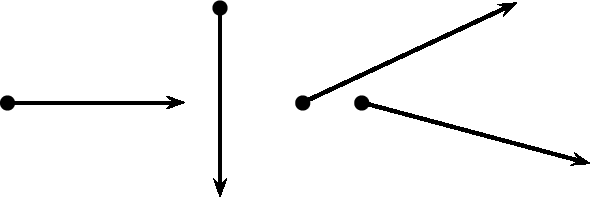
\includegraphics[width=5cm]{col11305.imgs/m38812_PG11C1_001.png} % m38812;PG11C1\_001.png;;;6.0;8.5;
        
      \vspace{2pt}
    \vspace{\rubberspace}\par \begin{cnxcaption}
	  \small \textbf{Figure 19.1: }Examples of vectors
	\end{cnxcaption}
      
    \vspace{.1in}
    \rule[.1in]{\figurerulewidth}{.005in} \\
        
    \end{center}

 \end{figure}   

    \addtocounter{footnote}{-0}
    
        
    \setcounter{subfigure}{0}


	\begin{figure}[H] % horizontal\label{m38812*uid4}
    \begin{center}
    \rule[.1in]{\figurerulewidth}{.005in} \\
        \label{m38812*uid4!!!underscore!!!media}\label{m38812*uid4!!!underscore!!!printimage}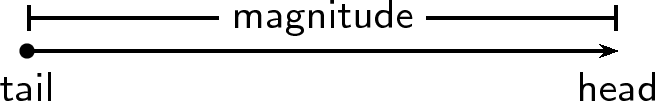
\includegraphics[width=6cm]{col11305.imgs/m38812_PG11C1_002.png} % m38812;PG11C1\_002.png;;;6.0;8.5;
        
      \vspace{2pt}
    \vspace{\rubberspace}\par \begin{cnxcaption}
	  \small \textbf{Figure 19.2: }Parts of a vector
	\end{cnxcaption}
      
    \vspace{.1in}
    \rule[.1in]{\figurerulewidth}{.005in} \\
        
    \end{center}

 \end{figure}   

    \addtocounter{footnote}{-0}
    
      
    
    \label{m38812*cid5}
            \subsection{ Directions}
            \nopagebreak
            
      
      \label{m38812*id187219}There are many acceptable methods of writing vectors. As long as the vector has a magnitude and a direction, it is most likely acceptable. These different methods come from the different methods of expressing a direction for a vector.\par 
      \label{m38812*uid5}
            \subsubsection{ Relative Directions}
            \nopagebreak
            
        
        \label{m38812*id187233}The simplest method of expressing direction is with relative directions: to the left, to the right, forward, backward, up and down.\par 
      
      \label{m38812*uid6}
            \subsubsection{ Compass Directions}
            \nopagebreak
            
        
        \label{m38812*id187246}Another common method of expressing directions is to use the points of a compass: North, South, East, and West.
If a vector does not point exactly in one of the compass directions, then we use an angle. For example, we can have a vector pointing \begin{math}40{}^{\circ }\end{math} North of West. Start with the vector pointing along the West direction:
Then rotate the vector towards the north until there is a \begin{math}40{}^{\circ }\end{math} angle between the vector and the West.
The direction of this vector can also be described as: W \begin{math}40{}^{\circ }\end{math} N (West \begin{math}40{}^{\circ }\end{math} North); or N \begin{math}50{}^{\circ }\end{math} W (North \begin{math}50{}^{\circ }\end{math} West)




    \setcounter{subfigure}{0}


	\begin{figure}[H] % horizontal\label{m38812*id187349}
    \begin{center}
    \label{m38812*id187349!!!underscore!!!media}\label{m38812*id187349!!!underscore!!!printimage}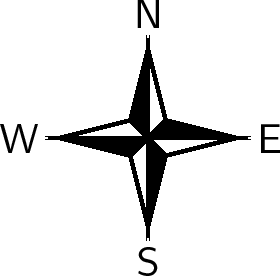
\includegraphics[width=2cm]{col11305.imgs/m38812_PG11C1_003.png} % m38812;PG11C1\_003.png;;;6.0;8.5;
        
      \vspace{2pt}
    \vspace{.1in}
    
    \end{center}

 \end{figure}   

    \addtocounter{footnote}{-0}
    
    \setcounter{subfigure}{0}


	\begin{figure}[H] % horizontal\label{m38812*id187358}
    \begin{center}
    \label{m38812*id187358!!!underscore!!!media}\label{m38812*id187358!!!underscore!!!printimage}
\includegraphics[width=3cm]{col11305.imgs/m38812_PG11C1_004.png} % m38812;PG11C1\_004.png;;;6.0;8.5;
        
      \vspace{2pt}
    \vspace{.1in}
    
    \end{center}

 \end{figure}   

    \addtocounter{footnote}{-0}
    
    \setcounter{subfigure}{0}


	\begin{figure}[H] % horizontal\label{m38812*id187367}
    \begin{center}
    \label{m38812*id187367!!!underscore!!!media}\label{m38812*id187367!!!underscore!!!printimage}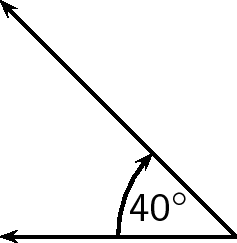
\includegraphics[width=3cm]{col11305.imgs/m38812_PG11C1_005.png} % m38812;PG11C1\_005.png;;;6.0;8.5;
        
      \vspace{2pt}
    \vspace{.1in}
    
    \end{center}

 \end{figure}   

    \addtocounter{footnote}{-0}
    \par 
      
      \label{m38812*uid7}
            \subsubsection{ Bearing}
            \nopagebreak
            
        
        \label{m38812*id187384}The final method of expressing direction is to use a \textsl{bearing}. A bearing is a direction relative to a fixed point.\par 
        \label{m38812*id187393}Given just an angle, the convention is to define the angle with respect to the North. So, a vector with a direction of \begin{math}110{}^{\circ }\end{math} has been rotated clockwise \begin{math}110{}^{\circ }\end{math} relative to the North. A bearing is always written as a three digit number, for example \begin{math}275{}^{\circ }\end{math} or \begin{math}080{}^{\circ }\end{math} (for \begin{math}80{}^{\circ }\end{math}).\par 
        \label{m38812*id187459}
          
    \setcounter{subfigure}{0}


	\begin{figure}[H] % horizontal\label{m38812*id187462}
    \begin{center}
    \label{m38812*id187462!!!underscore!!!media}\label{m38812*id187462!!!underscore!!!printimage}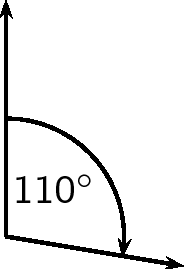
\includegraphics[width=3cm]{col11305.imgs/m38812_PG11C1_006.png} % m38812;PG11C1\_006.png;;;6.0;8.5;
        
      \vspace{2pt}
    \vspace{.1in}
    
    \end{center}

 \end{figure}   

    \addtocounter{footnote}{-0}
    
        \par 
\label{m38812*secfhsst!!!underscore!!!id146}
            \subsubsection{  Scalars and Vectors }
            \nopagebreak
            
        \label{m38812*id187475}\begin{enumerate}[noitemsep, label=\textbf{\arabic*}. ] 
            \label{m38812*uid8}\item Classify the following quantities as scalars or vectors:
\label{m38812*id187490}\begin{enumerate}[noitemsep, label=\textbf{\alph*}. ] 
            \label{m38812*uid9}\item 12 km
\label{m38812*uid10}\item 1 m south
\label{m38812*uid11}\item \begin{math}2\phantom{\rule{2pt}{0ex}}\mathrm{m}\ensuremath{\cdot}{\mathrm{s}}^{-1}\end{math}, \begin{math}45{}^{\circ }\end{math}\label{m38812*uid12}\item \begin{math}075{}^{\circ }\end{math}, 2 cm
\label{m38812*uid13}\item \begin{math}100\phantom{\rule{2pt}{0ex}}\mathrm{k}\ensuremath{\cdot}{\mathrm{h}}^{-1}\end{math}, \begin{math}0{}^{\circ }\end{math}\end{enumerate}
                \label{m38812*uid14}\item Use two different notations to write down the direction of the vector in each of the following diagrams:
\label{m38812*id187643}\begin{enumerate}[noitemsep, label=\textbf{\alph*}. ] 
            \label{m38812*uid15}\item 
    \setcounter{subfigure}{0}


	\begin{figure}[H] % horizontal\label{m38812*id187654}
    \begin{center}
    \label{m38812*id187654!!!underscore!!!media}\label{m38812*id187654!!!underscore!!!printimage}
\includegraphics[height=2cm]{col11305.imgs/m38812_PG11C1_007.png} % m38812;PG11C1\_007.png;;;6.0;8.5;
        
      \vspace{2pt}
    \vspace{.1in}
    
    \end{center}

 \end{figure}   

    \addtocounter{footnote}{-0}
    \label{m38812*uid16}\item 
    \setcounter{subfigure}{0}


	\begin{figure}[H] % horizontal\label{m38812*id187668}
    \begin{center}
    \label{m38812*id187668!!!underscore!!!media}\label{m38812*id187668!!!underscore!!!printimage}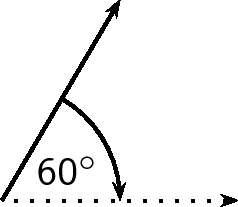
\includegraphics[width=3cm]{col11305.imgs/m38812_PG11C1_008.png} % m38812;PG11C1\_008.png;;;6.0;8.5;
        
      \vspace{2pt}
    \vspace{.1in}
    
    \end{center}

 \end{figure}   

    \addtocounter{footnote}{-0}
    \label{m38812*uid17}\item 
    \setcounter{subfigure}{0}


	\begin{figure}[H] % horizontal\label{m38812*id187683}
    \begin{center}
    \label{m38812*id187683!!!underscore!!!media}\label{m38812*id187683!!!underscore!!!printimage}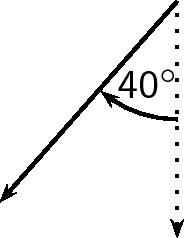
\includegraphics[width=3cm]{col11305.imgs/m38812_PG11C1_009.png} % m38812;PG11C1\_009.png;;;6.0;8.5;
        
      \vspace{2pt}
    \vspace{.1in}
    
    \end{center}

 \end{figure}   

    \addtocounter{footnote}{-0}
    \end{enumerate}
                \end{enumerate}
        
        

      
    
    \label{m38812*cid6}
\par \raisebox{-5 pt}{
\includegraphics[width=0.5cm]{col11305.imgs/summary_www.png}} Find the answers with the shortcodes:
 \par \begin{tabular}[h]{cccccc}
 (1.) l4s  &  (2.) l4H  & \end{tabular}



            \subsection{ Drawing Vectors}
            \nopagebreak
            
      
      \label{m38812*id187709}In order to draw a vector accurately we must specify a scale and
include a reference direction in the diagram. A scale allows us to
translate the length of the arrow into the vector's magnitude. For
instance if one chose a scale of 1 cm = 2 N (1 cm represents 2 N), a
force of 20 N towards the East would be represented as an arrow 10 cm
long. A reference direction may be a line representing a horizontal surface or the points of a compass.\par 
      \label{m38812*id187716}
        
    \setcounter{subfigure}{0}


	\begin{figure}[H] % horizontal\label{m38812*id187719}
    \begin{center}
    \label{m38812*id187719!!!underscore!!!media}\label{m38812*id187719!!!underscore!!!printimage}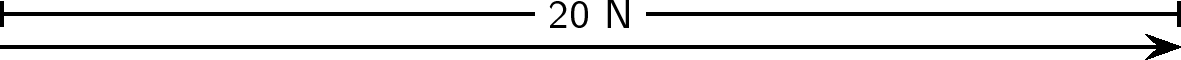
\includegraphics[width=5cm]{col11305.imgs/m38812_PG11C1_010.png} % m38812;PG11C1\_010.png;;;6.0;8.5;
        
      \vspace{2pt}
    \vspace{.1in}
    
    \end{center}

 \end{figure}   

    \addtocounter{footnote}{-0}
    
      \par 
      \label{m38812*id187725}
        \textbf{Method: Drawing Vectors}
        \label{m38812*id187736}\begin{enumerate}[noitemsep, label=\textbf{\arabic*}. ] 
            \label{m38812*uid18}\item Decide upon a scale and write it down.
\label{m38812*uid19}\item Determine the length of the arrow representing the vector, by using the scale.
\label{m38812*uid20}\item Draw the vector as an arrow. Make sure that you fill in the arrow head.
\label{m38812*uid21}\item Fill in the magnitude of the vector.
\end{enumerate}
        
      \par 
\par
            \label{m38812*secfhsst!!!underscore!!!id189}\vspace{.5cm} 
      
      \noindent
      \hspace*{-30pt}
\includegraphics[width=0.5in]{col11305.imgs/pspencil2.png}   \raisebox{25mm}{   
      \begin{mdframed}[linewidth=4, leftmargin=40, rightmargin=40]  
      \begin{exercise}
    \noindent\textbf{Exercise 19.1:  Drawing vectors }
      \label{m38812*probfhsst!!!underscore!!!id190}
      \label{m38812*id187800}Represent the following vector quantities:\par 
      \label{m38812*id187805}\begin{enumerate}[noitemsep, label=\textbf{\arabic*}. ] 
            \leftskip=20pt\rightskip=\leftskip\label{m38812*uid22}\item \begin{math}6\phantom{\rule{2pt}{0ex}}\mathrm{m}\ensuremath{\cdot}{\mathrm{s}}^{-1}\end{math} north
\label{m38812*uid23}\item 16 m east
\end{enumerate}
        
      
      \vspace{5pt}
      \label{m38812*solfhsst!!!underscore!!!id200}\noindent\textbf{Solution to Exercise } \label{m38812*listfhsst!!!underscore!!!id200}\begin{enumerate}[noitemsep, label=\textbf{Step} \textbf{\arabic*}. ] 
            \leftskip=20pt\rightskip=\leftskip\item  
      \label{m38812*id187874}\begin{enumerate}[noitemsep, label=\textbf{\alph*}. ] 
            \leftskip=20pt\rightskip=\leftskip\label{m38812*uid24}\item \begin{math}1\phantom{\rule{2pt}{0ex}}\mathrm{cm}=2\phantom{\rule{2pt}{0ex}}\mathrm{m}\ensuremath{\cdot}{\mathrm{s}}^{-1}\end{math}\label{m38812*uid25}\item \begin{math}1\phantom{\rule{2pt}{0ex}}\mathrm{cm}=4\phantom{\rule{2pt}{0ex}}\mathrm{m}\end{math}
\end{enumerate}
        
      \item  
      \label{m38812*id187925}\begin{enumerate}[noitemsep, label=\textbf{\alph*}. ] 
            \leftskip=20pt\rightskip=\leftskip\label{m38812*uid26}\item If \begin{math}1\phantom{\rule{2pt}{0ex}}\mathrm{cm}=2\phantom{\rule{2pt}{0ex}}\mathrm{m}\ensuremath{\cdot}{\mathrm{s}}^{-1}\end{math}, then \begin{math}6\phantom{\rule{2pt}{0ex}}\mathrm{m}\ensuremath{\cdot}{\mathrm{s}}^{-1}=3\phantom{\rule{2pt}{0ex}}\mathrm{cm}\end{math}
\label{m38812*uid27}\item If \begin{math}1\phantom{\rule{2pt}{0ex}}\mathrm{cm}=4\phantom{\rule{2pt}{0ex}}\mathrm{m}\end{math}, then \begin{math}16\phantom{\rule{2pt}{0ex}}\mathrm{m}=4\phantom{\rule{2pt}{0ex}}\mathrm{cm}\end{math}
\end{enumerate}
        
      \item  
      \label{m38812*id188000}\begin{enumerate}[noitemsep, label=\textbf{\alph*}. ] 
            \leftskip=20pt\rightskip=\leftskip\label{m38812*uid28}\item 
Scale used: \begin{math}1\phantom{\rule{2pt}{0ex}}\mathrm{cm}=2\phantom{\rule{2pt}{0ex}}\mathrm{m}\ensuremath{\cdot}{\mathrm{s}}^{-1}\end{math}
Direction = North

    \setcounter{subfigure}{0}


	\begin{figure}[H] % horizontal\label{m38812*id188039}
    \begin{center}
    \label{m38812*id188039!!!underscore!!!media}\label{m38812*id188039!!!underscore!!!printimage}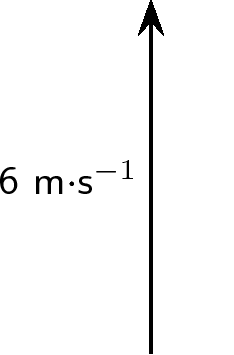
\includegraphics{col11305.imgs/m38812_PG11C1_011.png} % ;PG11C1\_011.png;;;6.0;8.5;
        
      \vspace{2pt}
    \vspace{.1in}
    
    \end{center}

 \end{figure}   

    \addtocounter{footnote}{-0}
    \label{m38812*uid29}\item 
Scale used: \begin{math}1\phantom{\rule{2pt}{0ex}}\mathrm{cm}=4\phantom{\rule{2pt}{0ex}}\mathrm{m}\end{math}
Direction = East

    \setcounter{subfigure}{0}


	\begin{figure}[H] % horizontal\label{m38812*id188060}
    \begin{center}
    \label{m38812*id188060!!!underscore!!!media}\label{m38812*id188060!!!underscore!!!printimage}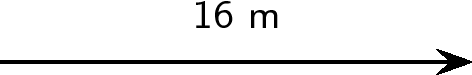
\includegraphics{col11305.imgs/m38812_PG11C1_012.png} % ;PG11C1\_012.png;;;6.0;8.5;
        
      \vspace{2pt}
    \vspace{.1in}
    
    \end{center}

 \end{figure}   

    \addtocounter{footnote}{-0}
    \end{enumerate}
        
      
      \end{enumerate}
         

    \end{exercise}
    \end{mdframed}
    }
    \noindent
  
\label{m38812*secfhsst!!!underscore!!!id228}
            \subsubsection{ Drawing Vectors }
            \nopagebreak
            \label{m38812*id188088}Draw each of the following vectors to scale. Indicate the scale that you have used:
      \label{m38812*id188094}\begin{enumerate}[noitemsep, label=\textbf{\arabic*}. ] 
            \label{m38812*uid30}\item 12 km south
\label{m38812*uid31}\item 1,5 m N \begin{math}45{}^{\circ }\end{math} W
\label{m38812*uid32}\item \begin{math}1\phantom{\rule{2pt}{0ex}}\mathrm{m}\ensuremath{\cdot}\mathrm{s}{}^{-1}\end{math}, \begin{math}20{}^{\circ }\end{math} East of North
\label{m38812*uid33}\item \begin{math}50\phantom{\rule{2pt}{0ex}}\mathrm{km}\ensuremath{\cdot}\mathrm{h}{}^{-1}\end{math}, \begin{math}085{}^{\circ }\end{math}\label{m38812*uid34}\item 5 mm, \begin{math}225{}^{\circ }\end{math}\end{enumerate}
                \par 
      

    

  \label{m38812**end}
          
\par \raisebox{-5 pt}{
\includegraphics[width=0.5cm]{col11305.imgs/summary_www.png}} Find the answers with the shortcodes:
 \par \begin{tabular}[h]{cccccc}
 (1.) l46  & \end{tabular}



         \section{ Mathematical properties}
    \nopagebreak
            \label{m38813} $ \hspace{-5pt}\begin{array}{cccccccccccc}   \end{array} $ \hspace{2 pt}\raisebox{-5 pt}{
\includegraphics[width=0.5cm]{col11305.imgs/summary_www.png}} {(section shortcode: P10092 )} \par 
    
    
    
    
    
    
  
    \label{m38813*cid7}
            \subsection{ Mathematical Properties of Vectors}
            \nopagebreak
            
      
      \label{m38813*id188277}Vectors are mathematical objects and we need to understand the mathematical properties of vectors, like adding and subtracting.\par 
      \label{m38813*id188281}For all the examples in this section, we will use displacement as our vector quantity. Displacement was discussed in
Grade 10.\par 
      \label{m38813*id188286}Displacement is defined as the distance together with direction of the straight line joining a final point to an initial point.\par 
      \label{m38813*id188290}Remember that displacement is just one example of a vector. We could just as well have decided to use forces or velocities to illustrate the properties of vectors.\par 
      \label{m38813*uid35}
            \subsubsection{ Adding Vectors}
            \nopagebreak
            
        
        \label{m38813*id188304}When vectors are added, we need to add both a magnitude \textbf{and} a direction. For example, take 2 steps in the forward direction, stop and then take another 3 steps in the forward direction. The first 2 steps is a displacement vector and the second 3 steps is also a displacement vector. If we did not stop after the first 2 steps, we would have taken 5 steps in the forward direction in total. Therefore, if we add the displacement vectors for 2 steps and 3 steps, we should get a total of 5 steps in the forward direction. Graphically, this can be seen by first following the first vector two steps forward and then following the second one three steps forward (ie. in the same direction):\par 
        \label{m38813*id188318}
          
    \setcounter{subfigure}{0}


	\begin{figure}[H] % horizontal\label{m38813*id188322}
    \begin{center}
    \label{m38813*id188322!!!underscore!!!media}\label{m38813*id188322!!!underscore!!!printimage}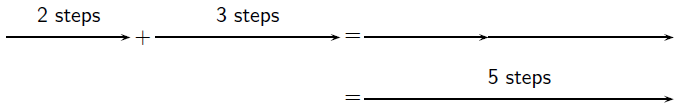
\includegraphics[width=300px]{col11305.imgs/m38813_PG11C1_013.png} % m38813;PG11C1\_013.png;;;6.0;8.5;
        
      \vspace{2pt}
    \vspace{.1in}
    
    \end{center}

 \end{figure}   

    \addtocounter{footnote}{-0}
    
        \par 
        \label{m38813*id188328}We add the second vector at the end of the first vector, since this is where we now are after the first vector has acted. The vector from the tail of the
first vector (the starting point) to the head of the last (the end
point) is then the sum of the vectors. This is the \textsl{head-to-tail} method of vector addition.\par 
        \label{m38813*id188340}As you can convince yourself, the order in which you add vectors does
not matter. In the example above, if you decided to first go 3 steps
forward and then another 2 steps forward, the end result would still be 5
steps forward.\par 
        \label{m38813*id188345}The final answer when adding vectors is called the \textbf{resultant}. The resultant displacement in this case will be 5 steps forward.\par 
\label{m38813*fhsst!!!underscore!!!id269}\begin{definition}
	  \begin{tabular*}{15 cm}{m{15 mm}m{}}
	\hspace*{-50pt}  
\includegraphics[width=0.5in]{col11305.imgs/psflag2.png}   & \Definition{   \label{id2512331}\textbf{ Resultant of Vectors }} { \label{m38813*meaningfhsst!!!underscore!!!id269}
        \label{m38813*id188362}The resultant of a number of vectors is the single vector whose effect is the same as the individual vectors acting together. \par 
         } 
      \end{tabular*}
      \end{definition}

        \label{m38813*id188374}In other words, the individual vectors can be replaced by the
resultant -- the overall effect is the same. If vectors \begin{math}\stackrel{\to }{a}\end{math} and \begin{math}\stackrel{\to }{b}\end{math} have a resultant \begin{math}\stackrel{\to }{R}\end{math}, this can be represented mathematically as,\par 
        \label{m38813*id188427}\nopagebreak\noindent{}
          \settowidth{\mymathboxwidth}{\begin{equation}
    \begin{array}{ccc}\hfill \stackrel{\to }{R}& =& \stackrel{\to }{a}+\stackrel{\to }{b}.\hfill \end{array}\tag{19.1}
      \end{equation}
    }
    \typeout{Columnwidth = \the\columnwidth}\typeout{math as usual width = \the\mymathboxwidth}
    \ifthenelse{\lengthtest{\mymathboxwidth < \columnwidth}}{% if the math fits, do it again, for real
    \begin{equation}
    \begin{array}{ccc}\hfill \stackrel{\to }{R}& =& \stackrel{\to }{a}+\stackrel{\to }{b}.\hfill \end{array}\tag{19.1}
      \end{equation}
    }{% else, if it doesn't fit
    \setlength{\mymathboxwidth}{\columnwidth}
      \addtolength{\mymathboxwidth}{-48pt}
    \par\vspace{12pt}\noindent\begin{minipage}{\columnwidth}
    \parbox[t]{\mymathboxwidth}{\large\begin{math}
    \stackrel{\to }{R}=\stackrel{\to }{a}+\stackrel{\to }{b}.\end{math}}\hfill
    \parbox[t]{48pt}{\raggedleft 
    (19.1)}
    \end{minipage}\vspace{12pt}\par
    }% end of conditional for this bit of math
    \typeout{math as usual width = \the\mymathboxwidth}
    
        
        \label{m38813*id188482}Let us consider some more examples of vector addition using displacements. The arrows tell you how far to move and in what
direction. Arrows to the right correspond to steps forward, while
arrows to the left correspond to steps backward. Look at all of the
examples below and check them.\par 
        \label{m38813*id186651}
          
    \setcounter{subfigure}{0}


	\begin{figure}[H] % horizontal\label{m38813*id186654}
    \begin{center}
    \label{m38813*id186654!!!underscore!!!media}\label{m38813*id186654!!!underscore!!!printimage}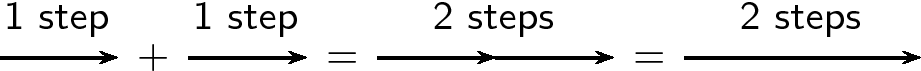
\includegraphics[width=300px]{col11305.imgs/m38813_PG11C1_014.png} % m38813;PG11C1\_014.png;;;6.0;8.5;
        
      \vspace{2pt}
    \vspace{.1in}
    
    \end{center}

 \end{figure}   

    \addtocounter{footnote}{-0}
    
        \par 
        \label{m38813*id186661}This example says 1 step forward and then another step forward is the same as an arrow twice as long -- two steps forward.\par 
        \label{m38813*id186668}
          
    \setcounter{subfigure}{0}


	\begin{figure}[H] % horizontal\label{m38813*id186672}
    \begin{center}
    \label{m38813*id186672!!!underscore!!!media}\label{m38813*id186672!!!underscore!!!printimage}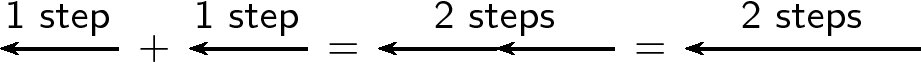
\includegraphics[width=300px]{col11305.imgs/m38813_PG11C1_015.png} % m38813;PG11C1\_015.png;;;6.0;8.5;
        
      \vspace{2pt}
    \vspace{.1in}
    
    \end{center}

 \end{figure}   

    \addtocounter{footnote}{-0}
    
        \par 
        \label{m38813*id186678}This examples says 1 step backward and then another step backward is the same as an arrow twice as long -- two steps backward.\par 
        \label{m38813*id186684}It is sometimes possible that you end up back where you started. In this case the net result of what you have done is that you have gone nowhere
(your start and end points are at the same place). In this case, your resultant displacement is a vector with length zero units. We use the symbol \begin{math}\stackrel{\to }{0}\end{math} to denote such a vector:\par 
        \label{m38813*id186706}
          
    \setcounter{subfigure}{0}


	\begin{figure}[H] % horizontal\label{m38813*id186710}
    \begin{center}
    \label{m38813*id186710!!!underscore!!!media}\label{m38813*id186710!!!underscore!!!printimage}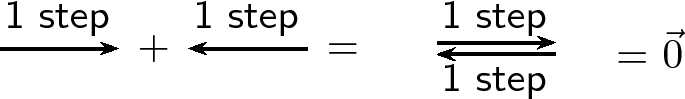
\includegraphics[width=6cm]{col11305.imgs/m38813_PG11C1_016.png} % m38813;PG11C1\_016.png;;;6.0;8.5;
        
      \vspace{2pt}
    \vspace{.1in}
    
    \end{center}

 \end{figure}   

    \addtocounter{footnote}{-0}
    
        \par 
        \label{m38813*id186716}
          
    \setcounter{subfigure}{0}


	\begin{figure}[H] % horizontal\label{m38813*id188625}
    \begin{center}
    \label{m38813*id188625!!!underscore!!!media}\label{m38813*id188625!!!underscore!!!printimage}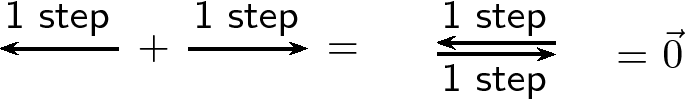
\includegraphics[width=6cm]{col11305.imgs/m38813_PG11C1_017.png} % m38813;PG11C1\_017.png;;;6.0;8.5;
        
      \vspace{2pt}
    \vspace{.1in}
    
    \end{center}

 \end{figure}   

    \addtocounter{footnote}{-0}
    
        \par 
        \label{m38813*id188632}Check the following examples in the same way. Arrows up the page can be
seen as steps left and arrows down the page as steps right.\par 
        \label{m38813*id188636}Try a couple to convince yourself!\par \nopagebreak
        
    % \textbf{m38813*id188639}\par
    
    % how many colspecs?  2
          % name: cnx:colspec
            % colnum: 1
            % colwidth: 10*
            % latex-name: columna
            % colname: 
            % align/tgroup-align/default: //left
            % -------------------------
            % name: cnx:colspec
            % colnum: 2
            % colwidth: 10*
            % latex-name: columnb
            % colname: 
            % align/tgroup-align/default: //left
            % -------------------------
      
    
    \setlength\mytablespace{4\tabcolsep}
    \addtolength\mytablespace{3\arrayrulewidth}
    \setlength\mytablewidth{\linewidth}
        
    
    \setlength\mytableroom{\mytablewidth}
    \addtolength\mytableroom{-\mytablespace}
    
    \setlength\myfixedwidth{0pt}
    \setlength\mystarwidth{\mytableroom}
        \addtolength\mystarwidth{-\myfixedwidth}
        \divide\mystarwidth 20
        
    
            % ----- Table with code
            
    % \begin{table}[H]
    % \\ '' '0'
    
        \begin{center}
      
      \label{m38813*id188639}
      
    \noindent
    \tabletail{%
        \hline
        \multicolumn{2}{|p{\mytableroom}|}{\raggedleft \small \sl continued on next page}\\
        \hline
      }
      \tablelasttail{}
      \begin{xtabular*}{\mytablewidth}[t]{|p{10\mystarwidth}|p{10\mystarwidth}|}\hline
    % count in rowspan-info-nodeset: 2
    % align/colidx: left,1
    
    % rowcount: '0' | start: 'false' | colidx: '1'
    
        % Formatting a regular cell and recurring on the next sibling
        
                  
    \setcounter{subfigure}{0}

\label{m38813*id188647}
    \begin{center}
    \label{m38813*id188647!!!underscore!!!media}\label{m38813*id188647!!!underscore!!!printimage}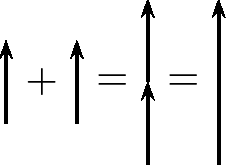
\includegraphics[width=3cm]{col11305.imgs/m38813_PG11C1_018.png} % m38813;PG11C1\_018.png;;;6.0;8.5;
        
      \vspace{2pt}
    \vspace{.1in}
    
    \end{center}



    \addtocounter{footnote}{-0}
    
                 &
      % align/colidx: left,2
    
    % rowcount: '0' | start: 'false' | colidx: '2'
    
        % Formatting a regular cell and recurring on the next sibling
        
                  
    \setcounter{subfigure}{0}

\label{m38813*id188657}
    \begin{center}
    \label{m38813*id188657!!!underscore!!!media}\label{m38813*id188657!!!underscore!!!printimage}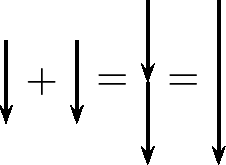
\includegraphics[width=3cm]{col11305.imgs/m38813_PG11C1_019.png} % m38813;PG11C1\_019.png;;;6.0;8.5;
        
      \vspace{2pt}
    \vspace{.1in}
    
    \end{center}



    \addtocounter{footnote}{-0}
    
                % make-rowspan-placeholders
    % rowspan info: col1 '0' | 'false' | '' || col2 '0' | 'false' | ''
     \tabularnewline\cline{1-1}\cline{2-2}
      %--------------------------------------------------------------------
    \end{xtabular*}
      \end{center}
    \begin{center}{\small\bfseries Table 19.1}\end{center}
    %\end{table}
    
    \addtocounter{footnote}{-0}
    
    \par
  
        
        
    % \textbf{m38813*id188668}\par
    
    % how many colspecs?  2
          % name: cnx:colspec
            % colnum: 1
            % colwidth: 10*
            % latex-name: columna
            % colname: 
            % align/tgroup-align/default: //left
            % -------------------------
            % name: cnx:colspec
            % colnum: 2
            % colwidth: 10*
            % latex-name: columnb
            % colname: 
            % align/tgroup-align/default: //left
            % -------------------------
      
    
    \setlength\mytablespace{4\tabcolsep}
    \addtolength\mytablespace{3\arrayrulewidth}
    \setlength\mytablewidth{\linewidth}
        
    
    \setlength\mytableroom{\mytablewidth}
    \addtolength\mytableroom{-\mytablespace}
    
    \setlength\myfixedwidth{0pt}
    \setlength\mystarwidth{\mytableroom}
        \addtolength\mystarwidth{-\myfixedwidth}
        \divide\mystarwidth 20
        
    
            % ----- Table with code
            
    % \begin{table}[H]
    % \\ '' '0'
    
        \begin{center}
      
      \label{m38813*id188668}
      
    \noindent
    \tabletail{%
        \hline
        \multicolumn{2}{|p{\mytableroom}|}{\raggedleft \small \sl continued on next page}\\
        \hline
      }
      \tablelasttail{}
      \begin{xtabular*}{\mytablewidth}[t]{|p{10\mystarwidth}|p{10\mystarwidth}|}\hline
    % count in rowspan-info-nodeset: 2
    % align/colidx: left,1
    
    % rowcount: '0' | start: 'false' | colidx: '1'
    
        % Formatting a regular cell and recurring on the next sibling
        
                  
    \setcounter{subfigure}{0}

\label{m38813*id188676}
    \begin{center}
    \label{m38813*id188676!!!underscore!!!media}\label{m38813*id188676!!!underscore!!!printimage}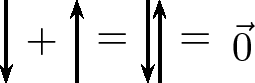
\includegraphics[width=3cm]{col11305.imgs/m38813_PG11C1_020.png} % m38813;PG11C1\_020.png;;;6.0;8.5;
        
      \vspace{2pt}
    \vspace{.1in}
    
    \end{center}



    \addtocounter{footnote}{-0}
    
                 &
      % align/colidx: left,2
    
    % rowcount: '0' | start: 'false' | colidx: '2'
    
        % Formatting a regular cell and recurring on the next sibling
        
                  
    \setcounter{subfigure}{0}

\label{m38813*id188686}
    \begin{center}
    \label{m38813*id188686!!!underscore!!!media}\label{m38813*id188686!!!underscore!!!printimage}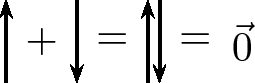
\includegraphics[width=3cm]{col11305.imgs/m38813_PG11C1_021.png} % m38813;PG11C1\_021.png;;;6.0;8.5;
        
      \vspace{2pt}
    \vspace{.1in}
    
    \end{center}



    \addtocounter{footnote}{-0}
    
                % make-rowspan-placeholders
    % rowspan info: col1 '0' | 'false' | '' || col2 '0' | 'false' | ''
     \tabularnewline\cline{1-1}\cline{2-2}
      %--------------------------------------------------------------------
    \end{xtabular*}
      \end{center}
    \begin{center}{\small\bfseries Table 19.2}\end{center}
    %\end{table}
    
    \addtocounter{footnote}{-0}
    
    \par
  
        
        \label{m38813*id188697}It is important to realise that the directions are not special-- `forward
and backwards' or `left and right' are treated in the same way. The same is
true of any set of parallel directions:\par 
        
    % \textbf{m38813*id188703}\par
    
    % how many colspecs?  2
          % name: cnx:colspec
            % colnum: 1
            % colwidth: 10*
            % latex-name: columna
            % colname: 
            % align/tgroup-align/default: //left
            % -------------------------
            % name: cnx:colspec
            % colnum: 2
            % colwidth: 10*
            % latex-name: columnb
            % colname: 
            % align/tgroup-align/default: //left
            % -------------------------
      
    
    \setlength\mytablespace{4\tabcolsep}
    \addtolength\mytablespace{3\arrayrulewidth}
    \setlength\mytablewidth{\linewidth}
        
    
    \setlength\mytableroom{\mytablewidth}
    \addtolength\mytableroom{-\mytablespace}
    
    \setlength\myfixedwidth{0pt}
    \setlength\mystarwidth{\mytableroom}
        \addtolength\mystarwidth{-\myfixedwidth}
        \divide\mystarwidth 20
        
    
            % ----- Table with code
            
    % \begin{table}[H]
    % \\ '' '0'
    
        \begin{center}
      
      \label{m38813*id188703}
      
    \noindent
    \tabletail{%
        \hline
        \multicolumn{2}{|p{\mytableroom}|}{\raggedleft \small \sl continued on next page}\\
        \hline
      }
      \tablelasttail{}
      \begin{xtabular*}{\mytablewidth}[t]{|p{10\mystarwidth}|p{10\mystarwidth}|}\hline
    % count in rowspan-info-nodeset: 2
    % align/colidx: left,1
    
    % rowcount: '0' | start: 'false' | colidx: '1'
    
        % Formatting a regular cell and recurring on the next sibling
        
                  
    \setcounter{subfigure}{0}

\label{m38813*id188711}
    \begin{center}
    \label{m38813*id188711!!!underscore!!!media}\label{m38813*id188711!!!underscore!!!printimage}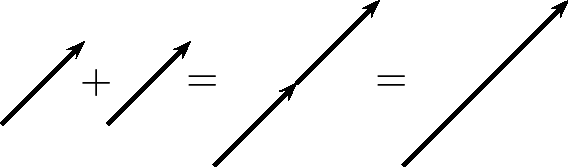
\includegraphics[width=3cm]{col11305.imgs/m38813_PG11C1_022.png} % m38813;PG11C1\_022.png;;;6.0;8.5;
        
      \vspace{2pt}
    \vspace{.1in}
    
    \end{center}



    \addtocounter{footnote}{-0}
    
                 &
      % align/colidx: left,2
    
    % rowcount: '0' | start: 'false' | colidx: '2'
    
        % Formatting a regular cell and recurring on the next sibling
        
                  
    \setcounter{subfigure}{0}

\label{m38813*id188721}
    \begin{center}
    \label{m38813*id188721!!!underscore!!!media}\label{m38813*id188721!!!underscore!!!printimage}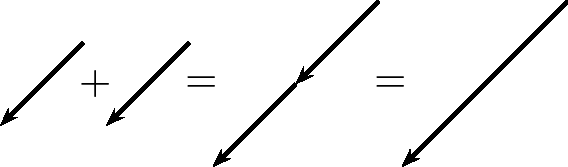
\includegraphics[width=3cm]{col11305.imgs/m38813_PG11C1_023.png} % m38813;PG11C1\_023.png;;;6.0;8.5;
        
      \vspace{2pt}
    \vspace{.1in}
    
    \end{center}



    \addtocounter{footnote}{-0}
    
                % make-rowspan-placeholders
    % rowspan info: col1 '0' | 'false' | '' || col2 '0' | 'false' | ''
     \tabularnewline\cline{1-1}\cline{2-2}
      %--------------------------------------------------------------------
    \end{xtabular*}
      \end{center}
    \begin{center}{\small\bfseries Table 19.3}\end{center}
    %\end{table}
    
    \addtocounter{footnote}{-0}
    
    \par
  
        
        
    % \textbf{m38813*id188732}\par
    
    % how many colspecs?  2
          % name: cnx:colspec
            % colnum: 1
            % colwidth: 10*
            % latex-name: columna
            % colname: 
            % align/tgroup-align/default: //left
            % -------------------------
            % name: cnx:colspec
            % colnum: 2
            % colwidth: 10*
            % latex-name: columnb
            % colname: 
            % align/tgroup-align/default: //left
            % -------------------------
      
    
    \setlength\mytablespace{4\tabcolsep}
    \addtolength\mytablespace{3\arrayrulewidth}
    \setlength\mytablewidth{\linewidth}
        
    
    \setlength\mytableroom{\mytablewidth}
    \addtolength\mytableroom{-\mytablespace}
    
    \setlength\myfixedwidth{0pt}
    \setlength\mystarwidth{\mytableroom}
        \addtolength\mystarwidth{-\myfixedwidth}
        \divide\mystarwidth 20
        
    
            % ----- Table with code
            
    % \begin{table}[H]
    % \\ '' '0'
    
        \begin{center}
      
      \label{m38813*id188732}
      
    \noindent
    \tabletail{%
        \hline
        \multicolumn{2}{|p{\mytableroom}|}{\raggedleft \small \sl continued on next page}\\
        \hline
      }
      \tablelasttail{}
      \begin{xtabular*}{\mytablewidth}[t]{|p{10\mystarwidth}|p{10\mystarwidth}|}\hline
    % count in rowspan-info-nodeset: 2
    % align/colidx: left,1
    
    % rowcount: '0' | start: 'false' | colidx: '1'
    
        % Formatting a regular cell and recurring on the next sibling
        
                  
    \setcounter{subfigure}{0}

\label{m38813*id188740}
    \begin{center}
    \label{m38813*id188740!!!underscore!!!media}\label{m38813*id188740!!!underscore!!!printimage}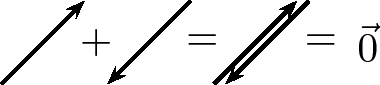
\includegraphics[width=3cm]{col11305.imgs/m38813_PG11C1_024.png} % m38813;PG11C1\_024.png;;;6.0;8.5;
        
      \vspace{2pt}
    \vspace{.1in}
    
    \end{center}



    \addtocounter{footnote}{-0}
    
                 &
      % align/colidx: left,2
    
    % rowcount: '0' | start: 'false' | colidx: '2'
    
        % Formatting a regular cell and recurring on the next sibling
        
                  
    \setcounter{subfigure}{0}

\label{m38813*id188750}
    \begin{center}
    \label{m38813*id188750!!!underscore!!!media}\label{m38813*id188750!!!underscore!!!printimage}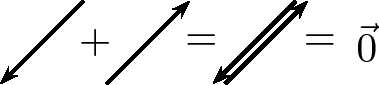
\includegraphics[width=3cm]{col11305.imgs/m38813_PG11C1_025.png} % m38813;PG11C1\_025.png;;;6.0;8.5;
        
      \vspace{2pt}
    \vspace{.1in}
    
    \end{center}



    \addtocounter{footnote}{-0}
    
                % make-rowspan-placeholders
    % rowspan info: col1 '0' | 'false' | '' || col2 '0' | 'false' | ''
     \tabularnewline\cline{1-1}\cline{2-2}
      %--------------------------------------------------------------------
    \end{xtabular*}
      \end{center}
    \begin{center}{\small\bfseries Table 19.4}\end{center}
    %\end{table}
    
    \addtocounter{footnote}{-0}
    
    \par
  
        
        \label{m38813*id188761}In the above examples the separate displacements were parallel to one
another. However the same head-to-tail technique of vector addition
can be applied to vectors in any direction.\par 
        
    % \textbf{m38813*id188766}\par
    
    % how many colspecs?  3
          % name: cnx:colspec
            % colnum: 1
            % colwidth: 10*
            % latex-name: columna
            % colname: 
            % align/tgroup-align/default: //left
            % -------------------------
            % name: cnx:colspec
            % colnum: 2
            % colwidth: 10*
            % latex-name: columnb
            % colname: 
            % align/tgroup-align/default: //left
            % -------------------------
            % name: cnx:colspec
            % colnum: 3
            % colwidth: 10*
            % latex-name: columnc
            % colname: 
            % align/tgroup-align/default: //left
            % -------------------------
      
    
    \setlength\mytablespace{6\tabcolsep}
    \addtolength\mytablespace{4\arrayrulewidth}
    \setlength\mytablewidth{\linewidth}
        
    
    \setlength\mytableroom{\mytablewidth}
    \addtolength\mytableroom{-\mytablespace}
    
    \setlength\myfixedwidth{0pt}
    \setlength\mystarwidth{\mytableroom}
        \addtolength\mystarwidth{-\myfixedwidth}
        \divide\mystarwidth 30
        
    
            % ----- Table with code
            
    % \begin{table}[H]
    % \\ '' '0'
    
        \begin{center}
      
      \label{m38813*id188766}
      
    \noindent
    \tabletail{%
        \hline
        \multicolumn{3}{|p{\mytableroom}|}{\raggedleft \small \sl continued on next page}\\
        \hline
      }
      \tablelasttail{}
      \begin{xtabular*}{\mytablewidth}[t]{|p{10\mystarwidth}|p{10\mystarwidth}|p{10\mystarwidth}|}\hline
    % count in rowspan-info-nodeset: 3
    % align/colidx: left,1
    
    % rowcount: '0' | start: 'false' | colidx: '1'
    
        % Formatting a regular cell and recurring on the next sibling
        
                  
    \setcounter{subfigure}{0}

\label{m38813*id188773}
    \begin{center}
    \label{m38813*id188773!!!underscore!!!media}\label{m38813*id188773!!!underscore!!!printimage}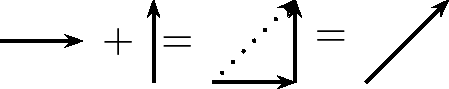
\includegraphics[width=3cm]{col11305.imgs/m38813_PG11C1_026.png} % m38813;PG11C1\_026.png;;;6.0;8.5;
        
      \vspace{2pt}
    \vspace{.1in}
    
    \end{center}



    \addtocounter{footnote}{-0}
    
                 &
      % align/colidx: left,2
    
    % rowcount: '0' | start: 'false' | colidx: '2'
    
        % Formatting a regular cell and recurring on the next sibling
        
                  
    \setcounter{subfigure}{0}

\label{m38813*id188783}
    \begin{center}
    \label{m38813*id188783!!!underscore!!!media}\label{m38813*id188783!!!underscore!!!printimage}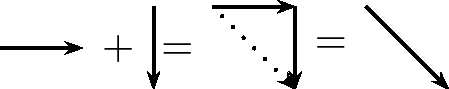
\includegraphics[width=3cm]{col11305.imgs/m38813_PG11C1_027.png} % m38813;PG11C1\_027.png;;;6.0;8.5;
        
      \vspace{2pt}
    \vspace{.1in}
    
    \end{center}



    \addtocounter{footnote}{-0}
    
                 &
      % align/colidx: left,3
    
    % rowcount: '0' | start: 'false' | colidx: '3'
    
        % Formatting a regular cell and recurring on the next sibling
        
                  
    \setcounter{subfigure}{0}

\label{m38813*id188793}
    \begin{center}
    \label{m38813*id188793!!!underscore!!!media}\label{m38813*id188793!!!underscore!!!printimage}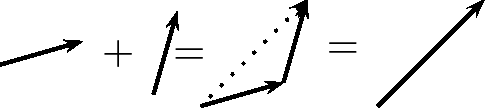
\includegraphics[width=3cm]{col11305.imgs/m38813_PG11C1_028.png} % m38813;PG11C1\_028.png;;;6.0;8.5;
        
      \vspace{2pt}
    \vspace{.1in}
    
    \end{center}



    \addtocounter{footnote}{-0}
    
                % make-rowspan-placeholders
    % rowspan info: col1 '0' | 'false' | '' || col2 '0' | 'false' | '' || col3 '0' | 'false' | ''
     \tabularnewline\cline{1-1}\cline{2-2}\cline{3-3}
      %--------------------------------------------------------------------
    \end{xtabular*}
      \end{center}
    \begin{center}{\small\bfseries Table 19.5}\end{center}
    %\end{table}
    
    \addtocounter{footnote}{-0}
    
    \par
  
        
        \label{m38813*id188804}Now you have discovered one use for vectors; describing resultant
displacement -- how far and in what direction you
have travelled after a series of movements.\par 
        \label{m38813*id188810}Although vector addition here has been demonstrated with
displacements, all vectors behave in exactly the same way. Thus, if
given a number of forces acting on a body you can use the same method
to determine the resultant force acting on the body. We will return to
vector addition in more detail later.\par 
      
      \label{m38813*uid36}
            \subsubsection{ Subtracting Vectors}
            \nopagebreak
            
        
        \label{m38813*id188826}What does it mean to subtract a vector? Well this is really simple; if
we have 5 apples and we subtract 3 apples, we have only 2 apples left. Now
lets work in steps; if we take 5 steps forward and then subtract 3 steps
forward we are left with only two steps forward:\par 
        \label{m38813*id188832}
    \setcounter{subfigure}{0}


	\begin{figure}[H] % horizontal\label{m38813*id188835}
    \begin{center}
    \label{m38813*id188835!!!underscore!!!media}\label{m38813*id188835!!!underscore!!!printimage}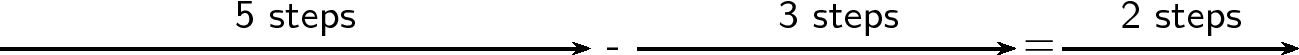
\includegraphics[width=8cm]{col11305.imgs/m38813_PG11C1_029.png} % m38813;PG11C1\_029.png;;;6.0;8.5;
        
      \vspace{2pt}
    \vspace{.1in}
    
    \end{center}

 \end{figure}   

    \addtocounter{footnote}{-0}
    
        \par 
        \label{m38813*id188842}What have we done? You originally took 5 steps forward but then you took
3 steps back. That backward displacement would be represented by an arrow
pointing to the left (backwards) with length 3. The net result of
adding these two vectors is 2 steps forward:\par 
        \label{m38813*id188847}
          
    \setcounter{subfigure}{0}


	\begin{figure}[H] % horizontal\label{m38813*id188851}
    \begin{center}
    \label{m38813*id188851!!!underscore!!!media}\label{m38813*id188851!!!underscore!!!printimage}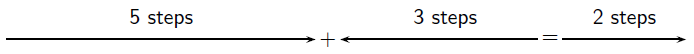
\includegraphics[width=8cm]{col11305.imgs/m38813_PG11C1_030.png} % m38813;PG11C1\_030.png;;;6.0;8.5;
        
      \vspace{2pt}
    \vspace{.1in}
    
    \end{center}

 \end{figure}   

    \addtocounter{footnote}{-0}
    
        \par 
        \label{m38813*id188857}Thus, subtracting a vector from another is the same as adding a vector in the opposite direction (i.e. subtracting 3 steps forwards is the same
as adding 3 steps backwards).\par 
\label{m38813*notfhsst!!!underscore!!!id524}
\begin{tabular}{cc}
	   \hspace*{-50pt}\raisebox{-8 mm}{ 
\includegraphics[width=0.5in]{col11305.imgs/pstip2.png}  }& 

	\begin{minipage}{0.85\textwidth}
	\begin{note}
      {tip: }Subtracting a vector from another is the same as adding a vector in the opposite direction.
	\end{note}
	\end{minipage}
	\end{tabular}
	\par
      
        \label{m38813*id188869}In the problem, motion in the forward direction has been represented by an arrow to the right. Arrows to the right are positive and arrows to the left are negative. More generally, vectors in opposite directions differ in sign (i.e. if we define up as positive, then
vectors acting down are negative). Thus, changing the sign of a vector
simply reverses its direction:\par 
        
    % \textbf{m38813*id188875}\par
    
    % how many colspecs?  2
          % name: cnx:colspec
            % colnum: 1
            % colwidth: 10*
            % latex-name: columna
            % colname: 
            % align/tgroup-align/default: //left
            % -------------------------
            % name: cnx:colspec
            % colnum: 2
            % colwidth: 10*
            % latex-name: columnb
            % colname: 
            % align/tgroup-align/default: //left
            % -------------------------
      
    
    \setlength\mytablespace{4\tabcolsep}
    \addtolength\mytablespace{3\arrayrulewidth}
    \setlength\mytablewidth{\linewidth}
        
    
    \setlength\mytableroom{\mytablewidth}
    \addtolength\mytableroom{-\mytablespace}
    
    \setlength\myfixedwidth{0pt}
    \setlength\mystarwidth{\mytableroom}
        \addtolength\mystarwidth{-\myfixedwidth}
        \divide\mystarwidth 20
        
    
            % ----- Table with code
            
    % \begin{table}[H]
    % \\ '' '0'
    
        \begin{center}
      
      \label{m38813*id188875}
      
    \noindent
    \tabletail{%
        \hline
        \multicolumn{2}{|p{\mytableroom}|}{\raggedleft \small \sl continued on next page}\\
        \hline
      }
      \tablelasttail{}
      \begin{xtabular*}{\mytablewidth}[t]{|p{10\mystarwidth}|p{10\mystarwidth}|}\hline
    % count in rowspan-info-nodeset: 2
    % align/colidx: left,1
    
    % rowcount: '0' | start: 'false' | colidx: '1'
    
        % Formatting a regular cell and recurring on the next sibling
        
                  
    \setcounter{subfigure}{0}

\label{m38813*id188883}
    \begin{center}
    \label{m38813*id188883!!!underscore!!!media}\label{m38813*id188883!!!underscore!!!printimage}
\includegraphics[width=3cm]{col11305.imgs/m38813_PG11C1_031.png} % m38813;PG11C1\_031.png;;;6.0;8.5;
        
      \vspace{2pt}
    \vspace{.1in}
    
    \end{center}



    \addtocounter{footnote}{-0}
    
                 &
      % align/colidx: left,2
    
    % rowcount: '0' | start: 'false' | colidx: '2'
    
        % Formatting a regular cell and recurring on the next sibling
        
                  
    \setcounter{subfigure}{0}

\label{m38813*id188893}
    \begin{center}
    \label{m38813*id188893!!!underscore!!!media}\label{m38813*id188893!!!underscore!!!printimage}
\includegraphics[width=3cm]{col11305.imgs/m38813_PG11C1_032.png} % m38813;PG11C1\_032.png;;;6.0;8.5;
        
      \vspace{2pt}
    \vspace{.1in}
    
    \end{center}



    \addtocounter{footnote}{-0}
    
                % make-rowspan-placeholders
    % rowspan info: col1 '0' | 'false' | '' || col2 '0' | 'false' | ''
     \tabularnewline\cline{1-1}\cline{2-2}
      %--------------------------------------------------------------------
    \end{xtabular*}
      \end{center}
    \begin{center}{\small\bfseries Table 19.6}\end{center}
    %\end{table}
    
    \addtocounter{footnote}{-0}
    
    \par
  
        
        
    % \textbf{m38813*id188904}\par
    
    % how many colspecs?  2
          % name: cnx:colspec
            % colnum: 1
            % colwidth: 10*
            % latex-name: columna
            % colname: 
            % align/tgroup-align/default: //left
            % -------------------------
            % name: cnx:colspec
            % colnum: 2
            % colwidth: 10*
            % latex-name: columnb
            % colname: 
            % align/tgroup-align/default: //left
            % -------------------------
      
    
    \setlength\mytablespace{4\tabcolsep}
    \addtolength\mytablespace{3\arrayrulewidth}
    \setlength\mytablewidth{\linewidth}
        
    
    \setlength\mytableroom{\mytablewidth}
    \addtolength\mytableroom{-\mytablespace}
    
    \setlength\myfixedwidth{0pt}
    \setlength\mystarwidth{\mytableroom}
        \addtolength\mystarwidth{-\myfixedwidth}
        \divide\mystarwidth 20
        
    
            % ----- Table with code
            
    % \begin{table}[H]
    % \\ '' '0'
    
        \begin{center}
      
      \label{m38813*id188904}
      
    \noindent
    \tabletail{%
        \hline
        \multicolumn{2}{|p{\mytableroom}|}{\raggedleft \small \sl continued on next page}\\
        \hline
      }
      \tablelasttail{}
      \begin{xtabular*}{\mytablewidth}[t]{|p{10\mystarwidth}|p{10\mystarwidth}|}\hline
    % count in rowspan-info-nodeset: 2
    % align/colidx: left,1
    
    % rowcount: '0' | start: 'false' | colidx: '1'
    
        % Formatting a regular cell and recurring on the next sibling
        
                  
    \setcounter{subfigure}{0}

\label{m38813*id188912}
    \begin{center}
    \label{m38813*id188912!!!underscore!!!media}\label{m38813*id188912!!!underscore!!!printimage}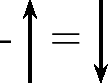
\includegraphics[width=3cm]{col11305.imgs/m38813_PG11C1_033.png} % m38813;PG11C1\_033.png;;;6.0;8.5;
        
      \vspace{2pt}
    \vspace{.1in}
    
    \end{center}



    \addtocounter{footnote}{-0}
    
                 &
      % align/colidx: left,2
    
    % rowcount: '0' | start: 'false' | colidx: '2'
    
        % Formatting a regular cell and recurring on the next sibling
        
                  
    \setcounter{subfigure}{0}

\label{m38813*id188922}
    \begin{center}
    \label{m38813*id188922!!!underscore!!!media}\label{m38813*id188922!!!underscore!!!printimage}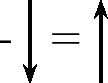
\includegraphics[width=3cm]{col11305.imgs/m38813_PG11C1_034.png} % m38813;PG11C1\_034.png;;;6.0;8.5;
        
      \vspace{2pt}
    \vspace{.1in}
    
    \end{center}



    \addtocounter{footnote}{-0}
    
                % make-rowspan-placeholders
    % rowspan info: col1 '0' | 'false' | '' || col2 '0' | 'false' | ''
     \tabularnewline\cline{1-1}\cline{2-2}
      %--------------------------------------------------------------------
    \end{xtabular*}
      \end{center}
    \begin{center}{\small\bfseries Table 19.7}\end{center}
    %\end{table}
    
    \addtocounter{footnote}{-0}
    
    \par
  
        
        
    % \textbf{m38813*id188933}\par
    
    % how many colspecs?  2
          % name: cnx:colspec
            % colnum: 1
            % colwidth: 10*
            % latex-name: columna
            % colname: 
            % align/tgroup-align/default: //left
            % -------------------------
            % name: cnx:colspec
            % colnum: 2
            % colwidth: 10*
            % latex-name: columnb
            % colname: 
            % align/tgroup-align/default: //left
            % -------------------------
      
    
    \setlength\mytablespace{4\tabcolsep}
    \addtolength\mytablespace{3\arrayrulewidth}
    \setlength\mytablewidth{\linewidth}
        
    
    \setlength\mytableroom{\mytablewidth}
    \addtolength\mytableroom{-\mytablespace}
    
    \setlength\myfixedwidth{0pt}
    \setlength\mystarwidth{\mytableroom}
        \addtolength\mystarwidth{-\myfixedwidth}
        \divide\mystarwidth 20
        
    
            % ----- Table with code
            
    % \begin{table}[H]
    % \\ '' '0'
    
        \begin{center}
      
      \label{m38813*id188933}
      
    \noindent
    \tabletail{%
        \hline
        \multicolumn{2}{|p{\mytableroom}|}{\raggedleft \small \sl continued on next page}\\
        \hline
      }
      \tablelasttail{}
      \begin{xtabular*}{\mytablewidth}[t]{|p{10\mystarwidth}|p{10\mystarwidth}|}\hline
    % count in rowspan-info-nodeset: 2
    % align/colidx: left,1
    
    % rowcount: '0' | start: 'false' | colidx: '1'
    
        % Formatting a regular cell and recurring on the next sibling
        
                  
    \setcounter{subfigure}{0}

\label{m38813*id188940}
    \begin{center}
    \label{m38813*id188940!!!underscore!!!media}\label{m38813*id188940!!!underscore!!!printimage}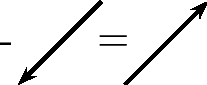
\includegraphics[width=3cm]{col11305.imgs/m38813_PG11C1_035.png} % m38813;PG11C1\_035.png;;;6.0;8.5;
        
      \vspace{2pt}
    \vspace{.1in}
    
    \end{center}



    \addtocounter{footnote}{-0}
    
                 &
      % align/colidx: left,2
    
    % rowcount: '0' | start: 'false' | colidx: '2'
    
        % Formatting a regular cell and recurring on the next sibling
        
                  
    \setcounter{subfigure}{0}

\label{m38813*id188950}
    \begin{center}
    \label{m38813*id188950!!!underscore!!!media}\label{m38813*id188950!!!underscore!!!printimage}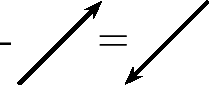
\includegraphics[width=3cm]{col11305.imgs/m38813_PG11C1_036.png} % m38813;PG11C1\_036.png;;;6.0;8.5;
        
      \vspace{2pt}
    \vspace{.1in}
    
    \end{center}



    \addtocounter{footnote}{-0}
    
                % make-rowspan-placeholders
    % rowspan info: col1 '0' | 'false' | '' || col2 '0' | 'false' | ''
     \tabularnewline\cline{1-1}\cline{2-2}
      %--------------------------------------------------------------------
    \end{xtabular*}
      \end{center}
    \begin{center}{\small\bfseries Table 19.8}\end{center}
    %\end{table}
    
    \addtocounter{footnote}{-0}
    
    \par
  
        
        \label{m38813*id188962}In mathematical form, subtracting \begin{math}\stackrel{\to }{a}\end{math} from
\begin{math}\stackrel{\to }{b}\end{math} gives a new vector \begin{math}\stackrel{\to }{c}\end{math}:\par 
        \label{m38813*id189012}\nopagebreak\noindent{}
          \settowidth{\mymathboxwidth}{\begin{equation}
    \begin{array}{ccc}\hfill \stackrel{\to }{c}& =& \stackrel{\to }{b}-\stackrel{\to }{a}\hfill \\ & =& \stackrel{\to }{b}+\left(-\stackrel{\to }{a}\right)\hfill \end{array}\tag{19.2}
      \end{equation}
    }
    \typeout{Columnwidth = \the\columnwidth}\typeout{math as usual width = \the\mymathboxwidth}
    \ifthenelse{\lengthtest{\mymathboxwidth < \columnwidth}}{% if the math fits, do it again, for real
    \begin{equation}
    \begin{array}{ccc}\hfill \stackrel{\to }{c}& =& \stackrel{\to }{b}-\stackrel{\to }{a}\hfill \\ & =& \stackrel{\to }{b}+\left(-\stackrel{\to }{a}\right)\hfill \end{array}\tag{19.2}
      \end{equation}
    }{% else, if it doesn't fit
    \setlength{\mymathboxwidth}{\columnwidth}
      \addtolength{\mymathboxwidth}{-48pt}
    \par\vspace{12pt}\noindent\begin{minipage}{\columnwidth}
    \parbox[t]{\mymathboxwidth}{\large\begin{math}
    \stackrel{\to }{c}=\stackrel{\to }{b}-\stackrel{\to }{a}=\stackrel{\to }{b}+\left(-\stackrel{\to }{a}\right)\end{math}}\hfill
    \parbox[t]{48pt}{\raggedleft 
    (19.2)}
    \end{minipage}\vspace{12pt}\par
    }% end of conditional for this bit of math
    \typeout{math as usual width = \the\mymathboxwidth}
    
        
        \label{m38813*id189102}This clearly shows that subtracting vector \begin{math}\stackrel{\to }{a}\end{math} from
\begin{math}\stackrel{\to }{b}\end{math} is the same as adding \begin{math}\left(-\stackrel{\to }{a}\right)\end{math} to
\begin{math}\stackrel{\to }{b}\end{math}. Look at the following examples of vector
subtraction.\par 
        \label{m38813*id189179}
          
    \setcounter{subfigure}{0}


	\begin{figure}[H] % horizontal\label{m38813*id189182}
    \begin{center}
    \label{m38813*id189182!!!underscore!!!media}\label{m38813*id189182!!!underscore!!!printimage}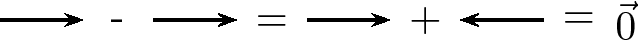
\includegraphics[width=6cm]{col11305.imgs/m38813_PG11C1_037.png} % m38813;PG11C1\_037.png;;;6.0;8.5;
        
      \vspace{2pt}
    \vspace{.1in}
    
    \end{center}

 \end{figure}   

    \addtocounter{footnote}{-0}
    
        \par 
        \label{m38813*id189188}
          
    \setcounter{subfigure}{0}


	\begin{figure}[H] % horizontal\label{m38813*id189192}
    \begin{center}
    \label{m38813*id189192!!!underscore!!!media}\label{m38813*id189192!!!underscore!!!printimage}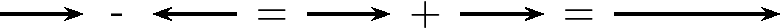
\includegraphics[width=6cm]{col11305.imgs/m38813_PG11C1_038.png} % m38813;PG11C1\_038.png;;;6.0;8.5;
        
      \vspace{2pt}
    \vspace{.1in}
    
    \end{center}

 \end{figure}   

    \addtocounter{footnote}{-0}
    
        \par 
      
      \label{m38813*uid37}
            \subsubsection{ Scalar Multiplication}
            \nopagebreak
            
        
        \label{m38813*id189208}What happens when you multiply a vector by a scalar (an ordinary
number)?\par 
        \label{m38813*id189212}Going back to normal multiplication we know that \begin{math}2\ensuremath{\times}2\end{math} is just
2 groups of 2 added together to give 4. We can adopt a similar approach to understand how vector multiplication works.\par 
        \label{m38813*id189232}
          
    \setcounter{subfigure}{0}


	\begin{figure}[H] % horizontal\label{m38813*id189235}
    \begin{center}
    \label{m38813*id189235!!!underscore!!!media}\label{m38813*id189235!!!underscore!!!printimage}
\includegraphics[width=300px]{col11305.imgs/m38813_PG11C1_039.png} % m38813;PG11C1\_039.png;;;6.0;8.5;
        
      \vspace{2pt}
    \vspace{.1in}
    
    \end{center}

 \end{figure}   

    \addtocounter{footnote}{-0}
    
        \par 
      
    

  \label{m38813**end}
          
         \section{ Techniques of vector addition}
    \nopagebreak
            \label{m38815} $ \hspace{-5pt}\begin{array}{cccccccccccc}   
\includegraphics[width=0.75cm]{col11305.imgs/summary_fullmarks.png} &   \end{array} $ \hspace{2 pt}\raisebox{-5 pt}{} {(section shortcode: P10093 )} \par 
    
    
    
    
    
    
  
    \label{m38815*cid8}
            \subsection{ Techniques of Vector Addition}
            \nopagebreak
            
      
      \label{m38815*id189251}Now that you have learned about the mathematical properties of
vectors, we return to vector addition in more detail. There are a number of
techniques of vector addition. These techniques fall into two main categories - graphical and algebraic techniques.\par 
      \label{m38815*uid38}
            \subsubsection{ Graphical Techniques}
            \nopagebreak
            
        
        \label{m38815*id189266}Graphical techniques involve drawing accurate scale diagrams to denote
individual vectors and their resultants. We next discuss the two primary
graphical techniques, the head-to-tail technique and the parallelogram
method.\par 
        \label{m38815*uid39}
            \subsubsection{ The Head-to-Tail Method}
            \nopagebreak
            
          
          \label{m38815*id189280}In describing the mathematical properties of vectors we used
displacements and the head-to-tail graphical method of vector addition
as an illustration. The head-to-tail method of graphically adding vectors is a standard method that must be understood.\par 
          \label{m38815*id189285}
            \textbf{Method: Head-to-Tail Method of Vector Addition}
          \par 
          \label{m38815*id189292}\begin{enumerate}[noitemsep, label=\textbf{\arabic*}. ] 
            \label{m38815*uid40}\item Draw a rough sketch of the situation.
\label{m38815*uid41}\item Choose a scale and include a reference direction.
\label{m38815*uid42}\item Choose any of the vectors and draw it as an arrow in the
correct direction and of the correct length -- remember to put an
arrowhead on the end to denote its direction.
\label{m38815*uid43}\item Take the next vector and draw it as an arrow starting from the
arrowhead of the first vector in the correct direction and of the
correct length.
\label{m38815*uid44}\item Continue until you have drawn each vector -- each time starting
from the head of the previous vector. In this way, the vectors to be
added are drawn one after the other head-to-tail.
\label{m38815*uid45}\item The resultant is then the vector drawn from the tail of the
first vector to the head of the last. Its magnitude can be
determined from the length of its arrow using the scale. Its
direction too can be determined from the scale diagram.
\end{enumerate}
        
\par
            \label{m38815*secfhsst!!!underscore!!!id738}\vspace{.5cm} 
      
      \noindent
      \hspace*{-30pt}
\includegraphics[width=0.5in]{col11305.imgs/pspencil2.png}   \raisebox{25mm}{   
      \begin{mdframed}[linewidth=4, leftmargin=40, rightmargin=40]  
      \begin{exercise}
    \noindent\textbf{Exercise 19.2: Head-to-Tail Addition I }\label{m38815*probfhsst!!!underscore!!!id739}
          \label{m38815*id189392}A ship leaves harbour H and sails 6 km north to port A. From here the ship travels 12 km east to port B, before sailing 5,5 km south-west to port C. Determine the ship's resultant displacement using the head-to-tail technique of vector addition. \par 
          \vspace{5pt}
          \label{m38815*solfhsst!!!underscore!!!id742}\noindent\textbf{Solution to Exercise } \label{m38815*listfhsst!!!underscore!!!id742}\begin{enumerate}[noitemsep, label=\textbf{Step} \textbf{\arabic*}. ] 
            \leftskip=20pt\rightskip=\leftskip\item  
          \label{m38815*id189417}Its easy to understand the problem if we first draw a quick sketch. The rough sketch should include all of the information given in the problem. All of the magnitudes of the displacements are shown and a compass has been included as a reference direction. In a rough sketch one is interested in the approximate shape of the vector diagram.\par 
          \label{m38815*id189423}
            
    \setcounter{subfigure}{0}


	\begin{figure}[H] % horizontal\label{m38815*id189427}
    \begin{center}
    \label{m38815*id189427!!!underscore!!!media}\label{m38815*id189427!!!underscore!!!printimage}\includegraphics{col11305.imgs/m38815_PG11C1_040.png} % ;PG11C1\_040.png;;;6.0;8.5;
        
      \vspace{2pt}
    \vspace{.1in}
    
    \end{center}

 \end{figure}   

    \addtocounter{footnote}{-0}
    
          \par 
          \item  
          \label{m38815*id189438}The choice of scale depends on the actual question -- you should choose a
scale such that your vector diagram fits the page.\par 
          \label{m38815*id189443}It is clear from the rough sketch that choosing a scale where 1~cm represents 2~km (scale: 1~cm = 2~km) would be a good choice in this
problem. The diagram will then take up a good fraction of an A4 page. We now start the accurate construction.\par 
          \item  
          \label{m38815*id189458}Starting at the harbour H we draw the first vector 3~cm long in the direction north.\par 
          \label{m38815*id189462}
            
    \setcounter{subfigure}{0}


	\begin{figure}[H] % horizontal\label{m38815*id189466}
    \begin{center}
    \label{m38815*id189466!!!underscore!!!media}\label{m38815*id189466!!!underscore!!!printimage}\includegraphics{col11305.imgs/m38815_PG11C1_041.png} % ;PG11C1\_041.png;;;6.0;8.5;
        
      \vspace{2pt}
    \vspace{.1in}
    
    \end{center}

 \end{figure}   

    \addtocounter{footnote}{-0}
    
          \par 
          \item  
\label{m38815*id63422}Take the next vector and draw it as an arrow starting from the
head of the first vector in the correct direction and of the
correct length. 
\par 
          \label{m38815*id189477}Since the ship is now at port A we draw the second vector 6~cm long starting from point A in the direction east.\par 
          \label{m38815*id189483}
            
    \setcounter{subfigure}{0}


	\begin{figure}[H] % horizontal\label{m38815*id189486}
    \begin{center}
    \label{m38815*id189486!!!underscore!!!media}\label{m38815*id189486!!!underscore!!!printimage}\includegraphics{col11305.imgs/m38815_PG11C1_042.png} % ;PG11C1\_042.png;;;6.0;8.5;
        
      \vspace{2pt}
    \vspace{.1in}
    
    \end{center}

 \end{figure}   

    \addtocounter{footnote}{-0}
    
          \par 
          \item  
\label{m38815*id6211}Take the next vector and draw it as an arrow starting from the
head of the second vector in the correct direction and of the
correct length. 
\par 
          \label{m38815*id189498}Since the ship is now at port B we draw the third vector 2,25~cm long starting from this point in the direction south-west. A protractor is required to measure the angle of 45\begin{math}{}^{\circ }\end{math}.\par 
          \label{m38815*id189518}
            
    \setcounter{subfigure}{0}


	\begin{figure}[H] % horizontal\label{m38815*id189521}
    \begin{center}
    \label{m38815*id189521!!!underscore!!!media}\label{m38815*id189521!!!underscore!!!printimage}\includegraphics{col11305.imgs/m38815_PG11C1_043.png} % ;PG11C1\_043.png;;;6.0;8.5;
        
      \vspace{2pt}
    \vspace{.1in}
    
    \end{center}

 \end{figure}   

    \addtocounter{footnote}{-0}
    
          \par 
          \item  
\label{m38815*id1342}The resultant is then the vector drawn from the tail of the
first vector to the head of the last. Its magnitude can be
determined from the length of its arrow using the scale. Its
direction too can be determined from the scale diagram.
\par 
          \label{m38815*id189533}As a final step we draw the resultant displacement from
the starting point (the harbour H) to the end point (port C). We use a
ruler to measure the length of this arrow and a protractor to determine its direction.\par 
          \label{m38815*id189538}
            
    \setcounter{subfigure}{0}


	\begin{figure}[H] % horizontal\label{m38815*id189541}
    \begin{center}
    \label{m38815*id189541!!!underscore!!!media}\label{m38815*id189541!!!underscore!!!printimage}\includegraphics{col11305.imgs/m38815_PG11C1_044.png} % ;PG11C1\_044.png;;;6.0;8.5;
        
      \vspace{2pt}
    \vspace{.1in}
    
    \end{center}

 \end{figure}   

    \addtocounter{footnote}{-0}
    
          \par 
          \item  
          \label{m38815*id189552}We now use the scale to convert the length of the resultant in the scale diagram to the actual displacement in the problem. Since we have chosen a scale of 1~cm = 2~km in this problem the resultant has a magnitude of 9,2~km. The direction can be specified in terms of the angle measured either as \begin{math}072,3{}^{\circ }\end{math} east of north or on a bearing of \begin{math}072,3{}^{\circ }\end{math}.\par 
          \item  
          \label{m38815*id189591}The resultant displacement of the ship is 9,2 km on a bearing of \begin{math}072,3{}^{\circ }\end{math}. \par 
          \end{enumerate}
         

    \end{exercise}
    \end{mdframed}
    }
    \noindent
  
\label{m38815*secfhsst!!!underscore!!!id814}\vspace{.5cm} 
      
      \noindent
      \hspace*{-30pt}\includegraphics[width=0.5in]{col11305.imgs/pspencil2.png}   \raisebox{25mm}{   
      \begin{mdframed}[linewidth=4, leftmargin=40, rightmargin=40]  
      \begin{exercise}
    \noindent\textbf{Exercise 19.3:  Head-to-Tail Graphical Addition II }
          \label{m38815*probfhsst!!!underscore!!!id815}
          \label{m38815*id189632}A man walks 40 m East, then 30 m North.\par 
          \label{m38815*id189638}\begin{enumerate}[noitemsep, label=\textbf{\arabic*}. ] 
            \leftskip=20pt\rightskip=\leftskip\label{m38815*uid46}\item What was the total distance he walked?
\label{m38815*uid47}\item What is his resultant displacement?
\end{enumerate}
        
          
          \vspace{5pt}
          \label{m38815*solfhsst!!!underscore!!!id825}\noindent\textbf{Solution to Exercise } \label{m38815*listfhsst!!!underscore!!!id825}\begin{enumerate}[noitemsep, label=\textbf{Step} \textbf{\arabic*}. ] 
            \leftskip=20pt\rightskip=\leftskip\item  
          \label{m38815*id189688}
            
    \setcounter{subfigure}{0}


	\begin{figure}[H] % horizontal\label{m38815*id189692}
    \begin{center}
    \label{m38815*id189692!!!underscore!!!media}\label{m38815*id189692!!!underscore!!!printimage}\includegraphics[width=5cm]{col11305.imgs/m38815_PG11C1_045.png} % ;PG11C1\_045.png;;;6.0;8.5;
        
      \vspace{2pt}
    \vspace{.1in}
    
    \end{center}

 \end{figure}   

    \addtocounter{footnote}{-0}
    
          \par 
          \item  
          \label{m38815*id189703}In the first part of his journey he traveled 40 m and in the second part he traveled 30 m. This gives us a total distance traveled of 40 m + 30 m = 70 m.\par 
          \item  
          \label{m38815*id189711}The man's resultant displacement is the \textbf{vector} from where he started to where he ended. It is the vector sum of his two separate displacements. We will use the head-to-tail method of accurate construction to find this vector.\par 
          \item  
          \label{m38815*id189726}A scale of 1 cm represents 10 m (1~cm = 10~m) is a good choice here. Now we can begin the process of construction.\par 
          \item  
          \label{m38815*id189736}We draw the first displacement as an arrow 4~cm long in an eastwards direction.\par 
          \label{m38815*id189740}
            
    \setcounter{subfigure}{0}


	\begin{figure}[H] % horizontal\label{m38815*id189744}
    \begin{center}
    \label{m38815*id189744!!!underscore!!!media}\label{m38815*id189744!!!underscore!!!printimage}\includegraphics{col11305.imgs/m38815_PG11C1_046.png} % ;PG11C1\_046.png;;;6.0;8.5;
        
      \vspace{2pt}
    \vspace{.1in}
    
    \end{center}

 \end{figure}   

    \addtocounter{footnote}{-0}
    
          \par 
          \item  
          \label{m38815*id189754}Starting from the head of the first vector we draw the second vector as an arrow 3~cm long in a northerly direction.\par 
          \label{m38815*id189760}
            
    \setcounter{subfigure}{0}


	\begin{figure}[H] % horizontal\label{m38815*id189763}
    \begin{center}
    \label{m38815*id189763!!!underscore!!!media}\label{m38815*id189763!!!underscore!!!printimage}\includegraphics[width=6cm]{col11305.imgs/m38815_PG11C1_047.png} % ;PG11C1\_047.png;;;6.0;8.5;
        
      \vspace{2pt}
    \vspace{.1in}
    
    \end{center}

 \end{figure}   

    \addtocounter{footnote}{-0}
    
          \par 
          \item  
          \label{m38815*id189774}Now we connect the starting point to the end point and
measure the length and direction of this arrow (the resultant).\par 
          \label{m38815*id189778}
            
    \setcounter{subfigure}{0}


	\begin{figure}[H] % horizontal\label{m38815*id189781}
    \begin{center}
    \label{m38815*id189781!!!underscore!!!media}\label{m38815*id189781!!!underscore!!!printimage}\includegraphics[width=6cm]{col11305.imgs/m38815_PG11C1_048.png} % ;PG11C1\_048.png;;;6.0;8.5;
        
      \vspace{2pt}
    \vspace{.1in}
    
    \end{center}

 \end{figure}   

    \addtocounter{footnote}{-0}
    
          \par 
          \item  
          \label{m38815*id189792}To find the direction you measure the angle between the resultant and the 40~m vector. You should get about 37\begin{math}{}^{\circ }\end{math}.\par 
          \item  
          \label{m38815*id189815}Finally we use the scale to convert the length of the resultant in
the scale diagram to the actual magnitude of the resultant
displacement. According to the chosen scale 1 cm = 10 m. Therefore 5 cm represents 50 m. The resultant displacement is then 50 m  \begin{math}37{}^{\circ }\end{math} north of east.
 \par 
          \end{enumerate}
         

    \end{exercise}
    \end{mdframed}
    }
    \noindent
  
        
        
      

  \label{m38815**end}
          
         \section{ Adding and subtracting vectors}
    \nopagebreak
            \label{m38816} $ \hspace{-5pt}\begin{array}{cccccccccccc}   \includegraphics[width=0.75cm]{col11305.imgs/summary_fullmarks.png} &   \end{array} $ \hspace{2 pt}\raisebox{-5 pt}{} {(section shortcode: P10094 )} \par 
    
    
    
    
    
    
  
      \label{m38816*uid55}
            \subsection{ Algebraic Addition and Subtraction of Vectors}
            \nopagebreak
            
        
        \label{m38816*uid56}
            \subsubsection{ Vectors in a Straight Line}
            \nopagebreak
            
          
          \label{m38816*id190264}Whenever you are faced with adding vectors acting in a straight line (i.e. some directed left and some right, or some acting up and others down) you can use a very simple algebraic technique:\par 
          \label{m38816*id190269}
            \textbf{Method: Addition/Subtraction of Vectors in a Straight Line}
          \par 
          \label{m38816*id190277}\begin{enumerate}[noitemsep, label=\textbf{\arabic*}. ] 
            \label{m38816*uid57}\item Choose a positive direction. As an example, for
situations involving displacements in the directions west and east, you
might choose west as your positive direction. In that case,
displacements east are negative.
\label{m38816*uid58}\item Next simply add (or subtract) the
magnitude of the vectors using the appropriate signs.
\label{m38816*uid59}\item As a final step the direction of the resultant should be included in
words (positive answers are in the positive direction, while negative
resultants are in the negative direction).
\end{enumerate}
        
          \label{m38816*id190321}Let us consider a few examples.\par 
\label{m38816*secfhsst!!!underscore!!!id999}\vspace{.5cm} 
      
      \noindent
      \hspace*{-30pt}\includegraphics[width=0.5in]{col11305.imgs/pspencil2.png}   \raisebox{25mm}{   
      \begin{mdframed}[linewidth=4, leftmargin=40, rightmargin=40]  
      \begin{exercise}
    \noindent\textbf{Exercise 19.4:  Adding vectors algebraically I }
          \label{m38816*probfhsst!!!underscore!!!id1000}
          \label{m38816*id190338}A tennis ball is rolled towards a wall which is 10~m away from the ball. If after striking the wall the ball rolls a further 2,5~m along the ground away from the wall, calculate algebraically the ball's resultant displacement. \par 
          \vspace{5pt}
          \label{m38816*solfhsst!!!underscore!!!id1003}\noindent\textbf{Solution to Exercise } \label{m38816*listfhsst!!!underscore!!!id1003}\begin{enumerate}[noitemsep, label=\textbf{Step} \textbf{\arabic*}. ] 
            \leftskip=20pt\rightskip=\leftskip\item  
          \label{m38816*id190365}
            
    \setcounter{subfigure}{0}


	\begin{figure}[H] % horizontal\label{m38816*id190368}
    \begin{center}
    \label{m38816*id190368!!!underscore!!!media}\label{m38816*id190368!!!underscore!!!printimage}\includegraphics{col11305.imgs/m38816_PG11C1_054.png} % ;PG11C1\_054.png;;;6.0;8.5;
        
      \vspace{2pt}
    \vspace{.1in}
    
    \end{center}

 \end{figure}   

    \addtocounter{footnote}{-0}
    
          \par 
          \item  
          \label{m38816*id190379}We know that the resultant displacement of the ball
(\begin{math}{\stackrel{\to }{x}}_{R}\end{math}) is equal to the sum of the ball's separate
displacements (\begin{math}{\stackrel{\to }{x}}_{1}\end{math} and \begin{math}{\stackrel{\to }{x}}_{2}\end{math}):\par 
          \label{m38816*id190446}\nopagebreak\noindent{}
            \settowidth{\mymathboxwidth}{\begin{equation}
    \begin{array}{ccc}\hfill {\stackrel{\to }{x}}_{R}& =& {\stackrel{\to }{x}}_{1}+{\stackrel{\to }{x}}_{2}\hfill \end{array}\tag{19.3}
      \end{equation}
    }
    \typeout{Columnwidth = \the\columnwidth}\typeout{math as usual width = \the\mymathboxwidth}
    \ifthenelse{\lengthtest{\mymathboxwidth < \columnwidth}}{% if the math fits, do it again, for real
    \begin{equation}
    \begin{array}{ccc}\hfill {\stackrel{\to }{x}}_{R}& =& {\stackrel{\to }{x}}_{1}+{\stackrel{\to }{x}}_{2}\hfill \end{array}\tag{19.3}
      \end{equation}
    }{% else, if it doesn't fit
    \setlength{\mymathboxwidth}{\columnwidth}
      \addtolength{\mymathboxwidth}{-48pt}
    \par\vspace{12pt}\noindent\begin{minipage}{\columnwidth}
    \parbox[t]{\mymathboxwidth}{\large\begin{math}
    {\stackrel{\to }{x}}_{R}={\stackrel{\to }{x}}_{1}+{\stackrel{\to }{x}}_{2}\end{math}}\hfill
    \parbox[t]{48pt}{\raggedleft 
    (19.3)}
    \end{minipage}\vspace{12pt}\par
    }% end of conditional for this bit of math
    \typeout{math as usual width = \the\mymathboxwidth}
    
          
          \label{m38816*id190515}Since the motion of the ball is in a straight line (i.e. the ball
moves towards and away from the wall), we can use the method of algebraic addition
just explained.\par 
          \item  
          \label{m38816*id190526}Let's choose the \textbf{positive} direction to be towards the wall. This means that the \textbf{negative} direction is away from the wall.\par 
          \item  
          \label{m38816*id190545}With right positive:\par 
          \label{m38816*id190549}\nopagebreak\noindent{}\settowidth{\mymathboxwidth}{\begin{equation}
    \begin{array}{ccc}\hfill {\stackrel{\to }{x}}_{1}& =& +10,0\phantom{\rule{2pt}{0ex}}\mathrm{m}\ensuremath{\cdot}{\mathrm{s}}^{-1}\hfill \\ \hfill {\stackrel{\to }{x}}_{2}& =& -2,5\phantom{\rule{2pt}{0ex}}\mathrm{m}\ensuremath{\cdot}{\mathrm{s}}^{-1}\hfill \end{array}\tag{19.4}
      \end{equation}
    }
    \typeout{Columnwidth = \the\columnwidth}\typeout{math as usual width = \the\mymathboxwidth}
    \ifthenelse{\lengthtest{\mymathboxwidth < \columnwidth}}{% if the math fits, do it again, for real
    \begin{equation}
    \begin{array}{ccc}\hfill {\stackrel{\to }{x}}_{1}& =& +10,0\phantom{\rule{2pt}{0ex}}\mathrm{m}\ensuremath{\cdot}{\mathrm{s}}^{-1}\hfill \\ \hfill {\stackrel{\to }{x}}_{2}& =& -2,5\phantom{\rule{2pt}{0ex}}\mathrm{m}\ensuremath{\cdot}{\mathrm{s}}^{-1}\hfill \end{array}\tag{19.4}
      \end{equation}
    }{% else, if it doesn't fit
    \setlength{\mymathboxwidth}{\columnwidth}
      \addtolength{\mymathboxwidth}{-48pt}
    \par\vspace{12pt}\noindent\begin{minipage}{\columnwidth}
    \parbox[t]{\mymathboxwidth}{\large\begin{math}
    {\stackrel{\to }{x}}_{1}=+10,0\phantom{\rule{2pt}{0ex}}\mathrm{m}\ensuremath{\cdot}{\mathrm{s}}^{-1}{\stackrel{\to }{x}}_{2}=-2,5\phantom{\rule{2pt}{0ex}}\mathrm{m}\ensuremath{\cdot}{\mathrm{s}}^{-1}\end{math}}\hfill
    \parbox[t]{48pt}{\raggedleft 
    (19.4)}
    \end{minipage}\vspace{12pt}\par
    }% end of conditional for this bit of math
    \typeout{math as usual width = \the\mymathboxwidth}
    
          
          \item  
          \label{m38816*id190665}Next we simply add the two displacements to give the resultant:\par 
          \label{m38816*id190669}\nopagebreak\noindent{}\settowidth{\mymathboxwidth}{\begin{equation}
    \begin{array}{ccc}\hfill {\stackrel{\to }{x}}_{R}& =& \left(+10\phantom{\rule{2pt}{0ex}}\mathrm{m}\ensuremath{\cdot}{\mathrm{s}}^{-1}\right)+\left(-2,5\phantom{\rule{2pt}{0ex}}\mathrm{m}\ensuremath{\cdot}{\mathrm{s}}^{-1}\right)\hfill \\ & =& \left(+7,5\right)\phantom{\rule{2pt}{0ex}}\mathrm{m}\ensuremath{\cdot}{\mathrm{s}}^{-1}\hfill \end{array}\tag{19.5}
      \end{equation}
    }
    \typeout{Columnwidth = \the\columnwidth}\typeout{math as usual width = \the\mymathboxwidth}
    \ifthenelse{\lengthtest{\mymathboxwidth < \columnwidth}}{% if the math fits, do it again, for real
    \begin{equation}
    \begin{array}{ccc}\hfill {\stackrel{\to }{x}}_{R}& =& \left(+10\phantom{\rule{2pt}{0ex}}\mathrm{m}\ensuremath{\cdot}{\mathrm{s}}^{-1}\right)+\left(-2,5\phantom{\rule{2pt}{0ex}}\mathrm{m}\ensuremath{\cdot}{\mathrm{s}}^{-1}\right)\hfill \\ & =& \left(+7,5\right)\phantom{\rule{2pt}{0ex}}\mathrm{m}\ensuremath{\cdot}{\mathrm{s}}^{-1}\hfill \end{array}\tag{19.5}
      \end{equation}
    }{% else, if it doesn't fit
    \setlength{\mymathboxwidth}{\columnwidth}
      \addtolength{\mymathboxwidth}{-48pt}
    \par\vspace{12pt}\noindent\begin{minipage}{\columnwidth}
    \parbox[t]{\mymathboxwidth}{\large\begin{math}
    {\stackrel{\to }{x}}_{R}=\left(+10\phantom{\rule{2pt}{0ex}}\mathrm{m}\ensuremath{\cdot}{\mathrm{s}}^{-1}\right)+\left(-2,5\phantom{\rule{2pt}{0ex}}\mathrm{m}\ensuremath{\cdot}{\mathrm{s}}^{-1}\right)=\left(+7,5\right)\phantom{\rule{2pt}{0ex}}\mathrm{m}\ensuremath{\cdot}{\mathrm{s}}^{-1}\end{math}}\hfill
    \parbox[t]{48pt}{\raggedleft 
    (19.5)}
    \end{minipage}\vspace{12pt}\par
    }% end of conditional for this bit of math
    \typeout{math as usual width = \the\mymathboxwidth}
    
          
          \item  
          \label{m38816*id190806}Finally, in this case \uline{towards the wall is the positive direction}, so:
\begin{math}{\stackrel{\to }{x}}_{R}\end{math} = 7,5 m towards the wall. \par 
          \end{enumerate}
         

    \end{exercise}
    \end{mdframed}
    }
    \noindent
  
\label{m38816*secfhsst!!!underscore!!!id1222}\vspace{.5cm} 
      
      \noindent
      \hspace*{-30pt}\includegraphics[width=0.5in]{col11305.imgs/pspencil2.png}   \raisebox{25mm}{   
      \begin{mdframed}[linewidth=4, leftmargin=40, rightmargin=40]  
      \begin{exercise}
    \noindent\textbf{Exercise 19.5:  Subtracting vectors algebraically I }
          \label{m38816*probfhsst!!!underscore!!!id1223}
          \label{m38816*id190861}Suppose that a tennis ball is thrown horizontally towards a wall at an initial velocity of \begin{math}3\phantom{\rule{2pt}{0ex}}\mathrm{m}\ensuremath{\cdot}\mathrm{s}{}^{-1}\end{math} to the right. After striking the wall, the ball returns to the thrower at  \begin{math}2\phantom{\rule{2pt}{0ex}}\mathrm{m}\ensuremath{\cdot}\mathrm{s}{}^{-1}\end{math}. Determine the change in velocity of the ball. \par 
          \vspace{5pt}
          \label{m38816*solfhsst!!!underscore!!!id1226}\noindent\textbf{Solution to Exercise } \label{m38816*listfhsst!!!underscore!!!id1226}\begin{enumerate}[noitemsep, label=\textbf{Step} \textbf{\arabic*}. ] 
            \leftskip=20pt\rightskip=\leftskip\item  
          \label{m38816*id190936}A quick sketch will help us understand the problem.\par 
          \label{m38816*id190940}
            
    \setcounter{subfigure}{0}


	\begin{figure}[H] % horizontal\label{m38816*id190944}
    \begin{center}
    \label{m38816*id190944!!!underscore!!!media}\label{m38816*id190944!!!underscore!!!printimage}\includegraphics{col11305.imgs/m38816_PG11C1_055.png} % ;PG11C1\_055.png;;;6.0;8.5;
        
      \vspace{2pt}
    \vspace{.1in}
    
    \end{center}

 \end{figure}   

    \addtocounter{footnote}{-0}
    
          \par 
          \item  
          \label{m38816*id190954}Remember that velocity is a vector. The change in the velocity of the
ball is equal to the difference between the ball's initial and final
velocities:\par 
          \label{m38816*id190959}\nopagebreak\noindent{}
            \settowidth{\mymathboxwidth}{\begin{equation}
    \Delta \stackrel{\to }{v}={\stackrel{\to }{v}}_{f}-{\stackrel{\to }{v}}_{i}\tag{19.6}
      \end{equation}
    }
    \typeout{Columnwidth = \the\columnwidth}\typeout{math as usual width = \the\mymathboxwidth}
    \ifthenelse{\lengthtest{\mymathboxwidth < \columnwidth}}{% if the math fits, do it again, for real
    \begin{equation}
    \Delta \stackrel{\to }{v}={\stackrel{\to }{v}}_{f}-{\stackrel{\to }{v}}_{i}\tag{19.6}
      \end{equation}
    }{% else, if it doesn't fit
    \setlength{\mymathboxwidth}{\columnwidth}
      \addtolength{\mymathboxwidth}{-48pt}
    \par\vspace{12pt}\noindent\begin{minipage}{\columnwidth}
    \parbox[t]{\mymathboxwidth}{\large\begin{math}
    \Delta \stackrel{\to }{v}={\stackrel{\to }{v}}_{f}-{\stackrel{\to }{v}}_{i}\end{math}}\hfill
    \parbox[t]{48pt}{\raggedleft 
    (19.6)}
    \end{minipage}\vspace{12pt}\par
    }% end of conditional for this bit of math
    \typeout{math as usual width = \the\mymathboxwidth}
    
          
          \label{m38816*id191013}Since the ball moves along a straight line (i.e. left and right), we
can use the algebraic technique of vector subtraction just discussed.\par 
          \item  
          \label{m38816*id191022}Choose the \textbf{positive} direction to be towards the wall. This means that the \textbf{negative} direction is away from the wall.\par 
          \item  
          \label{m38816*id191042}\nopagebreak\noindent{}
            \settowidth{\mymathboxwidth}{\begin{equation}
    \begin{array}{ccc}\hfill {\stackrel{\to }{v}}_{i}& =& +3\phantom{\rule{2pt}{0ex}}\mathrm{m}\ensuremath{\cdot}{\mathrm{s}}^{-1}\hfill \\ \hfill {\stackrel{\to }{v}}_{f}& =& -2\phantom{\rule{2pt}{0ex}}\mathrm{m}\ensuremath{\cdot}{\mathrm{s}}^{-1}\hfill \end{array}\tag{19.7}
      \end{equation}
    }
    \typeout{Columnwidth = \the\columnwidth}\typeout{math as usual width = \the\mymathboxwidth}
    \ifthenelse{\lengthtest{\mymathboxwidth < \columnwidth}}{% if the math fits, do it again, for real
    \begin{equation}
    \begin{array}{ccc}\hfill {\stackrel{\to }{v}}_{i}& =& +3\phantom{\rule{2pt}{0ex}}\mathrm{m}\ensuremath{\cdot}{\mathrm{s}}^{-1}\hfill \\ \hfill {\stackrel{\to }{v}}_{f}& =& -2\phantom{\rule{2pt}{0ex}}\mathrm{m}\ensuremath{\cdot}{\mathrm{s}}^{-1}\hfill \end{array}\tag{19.7}
      \end{equation}
    }{% else, if it doesn't fit
    \setlength{\mymathboxwidth}{\columnwidth}
      \addtolength{\mymathboxwidth}{-48pt}
    \par\vspace{12pt}\noindent\begin{minipage}{\columnwidth}
    \parbox[t]{\mymathboxwidth}{\large\begin{math}
    {\stackrel{\to }{v}}_{i}=+3\phantom{\rule{2pt}{0ex}}\mathrm{m}\ensuremath{\cdot}{\mathrm{s}}^{-1}{\stackrel{\to }{v}}_{f}=-2\phantom{\rule{2pt}{0ex}}\mathrm{m}\ensuremath{\cdot}{\mathrm{s}}^{-1}\end{math}}\hfill
    \parbox[t]{48pt}{\raggedleft 
    (19.7)}
    \end{minipage}\vspace{12pt}\par
    }% end of conditional for this bit of math
    \typeout{math as usual width = \the\mymathboxwidth}
    
          
          \item  
          \label{m38816*id191149}Thus, the change in velocity of the ball is:\par 
          \label{m38816*id191153}\nopagebreak\noindent{}
            \settowidth{\mymathboxwidth}{\begin{equation}
    \begin{array}{ccc}\hfill \Delta \stackrel{\to }{v}& =& \left(-2\phantom{\rule{2pt}{0ex}}\mathrm{m}\ensuremath{\cdot}{\mathrm{s}}^{-1}\right)-\left(+3\phantom{\rule{2pt}{0ex}}\mathrm{m}\ensuremath{\cdot}{\mathrm{s}}^{-1}\right)\hfill \\ & =& \left(-5\right)\phantom{\rule{2pt}{0ex}}\mathrm{m}\ensuremath{\cdot}{\mathrm{s}}^{-1}\hfill \end{array}\tag{19.8}
      \end{equation}
    }
    \typeout{Columnwidth = \the\columnwidth}\typeout{math as usual width = \the\mymathboxwidth}
    \ifthenelse{\lengthtest{\mymathboxwidth < \columnwidth}}{% if the math fits, do it again, for real
    \begin{equation}
    \begin{array}{ccc}\hfill \Delta \stackrel{\to }{v}& =& \left(-2\phantom{\rule{2pt}{0ex}}\mathrm{m}\ensuremath{\cdot}{\mathrm{s}}^{-1}\right)-\left(+3\phantom{\rule{2pt}{0ex}}\mathrm{m}\ensuremath{\cdot}{\mathrm{s}}^{-1}\right)\hfill \\ & =& \left(-5\right)\phantom{\rule{2pt}{0ex}}\mathrm{m}\ensuremath{\cdot}{\mathrm{s}}^{-1}\hfill \end{array}\tag{19.8}
      \end{equation}
    }{% else, if it doesn't fit
    \setlength{\mymathboxwidth}{\columnwidth}
      \addtolength{\mymathboxwidth}{-48pt}
    \par\vspace{12pt}\noindent\begin{minipage}{\columnwidth}
    \parbox[t]{\mymathboxwidth}{\large\begin{math}
    \Delta \stackrel{\to }{v}=\left(-2\phantom{\rule{2pt}{0ex}}\mathrm{m}\ensuremath{\cdot}{\mathrm{s}}^{-1}\right)-\left(+3\phantom{\rule{2pt}{0ex}}\mathrm{m}\ensuremath{\cdot}{\mathrm{s}}^{-1}\right)=\left(-5\right)\phantom{\rule{2pt}{0ex}}\mathrm{m}\ensuremath{\cdot}{\mathrm{s}}^{-1}\end{math}}\hfill
    \parbox[t]{48pt}{\raggedleft 
    (19.8)}
    \end{minipage}\vspace{12pt}\par
    }% end of conditional for this bit of math
    \typeout{math as usual width = \the\mymathboxwidth}
    
          
          \item  
          \label{m38816*id191279}Remember that in this case \uline{towards the wall means a positive velocity}, so \uline{away from the wall means a negative velocity}:
\begin{math}\Delta \stackrel{\to }{v}=5\phantom{\rule{2pt}{0ex}}\mathrm{m}\ensuremath{\cdot}{\mathrm{s}}^{-1}\end{math} away from the wall. \par 
          \end{enumerate}
         

    \end{exercise}
    \end{mdframed}
    }
    \noindent
  
\label{m38816*secfhsst!!!underscore!!!id1424}
            \subsubsection{  Resultant Vectors }
            \nopagebreak
            
          \label{m38816*id191353}\begin{enumerate}[noitemsep, label=\textbf{\arabic*}. ] 
            \label{m38816*uid60}\item Harold walks to school by walking 600 m Northeast and then 500 m N \begin{math}40{}^{\circ }\end{math} W. Determine his resultant displacement by using accurate scale drawings.\newline
            
\label{m38816*uid61}\item A dove flies from her nest, looking for food for her chick. She flies at a velocity of \begin{math}2\mathrm{m}\ensuremath{\cdot}\mathrm{s}{}^{-1}\end{math} on a bearing of \begin{math}135{}^{\circ }\end{math} and then at a velocity of \begin{math}1,2\phantom{\rule{2pt}{0ex}}\mathrm{m}\ensuremath{\cdot}\mathrm{s}{}^{-1}\end{math} on a bearing of \begin{math}230{}^{\circ }\end{math}. Calculate her resultant velocity by using accurate scale drawings.\newline
            
\label{m38816*uid62}\item A squash ball is dropped to the floor with an initial velocity of \begin{math}2,5\phantom{\rule{2pt}{0ex}}\mathrm{m}\ensuremath{\cdot}\mathrm{s}{}^{-1}\end{math}. It rebounds (comes back up) with a velocity of \begin{math}0,5\phantom{\rule{2pt}{0ex}}\mathrm{m}\ensuremath{\cdot}\mathrm{s}{}^{-1}\end{math}.
\label{m38816*id191536}\begin{enumerate}[noitemsep, label=\textbf{\alph*}. ] 
            \label{m38816*uid63}\item What is the change in velocity of the squash ball?
\label{m38816*uid64}\item What is the resultant velocity of the squash ball?
\end{enumerate}
                \end{enumerate}
        
          

          \label{m38816*id191575}Remember that the technique of addition and subtraction just discussed can only be applied to vectors acting along a straight line. When vectors are not in a straight line, i.e. at an angle to each other, the following method can be used:\par 
        
        \label{m38816*uid65}
\par \raisebox{-5 pt}{\includegraphics[width=0.5cm]{col11305.imgs/summary_www.png}} Find the answers with the shortcodes:
 \par \begin{tabular}[h]{cccccc}
 (1.) l2b  &  (2.) l2j  &  (3.) l4F  & \end{tabular}



            \subsubsection{ A More General Algebraic technique}
            \nopagebreak
            
          
          \label{m38816*id191590}Simple geometric and trigonometric techniques can be used to find resultant vectors.\par 
\label{m38816*secfhsst!!!underscore!!!id1442}\vspace{.5cm} 
      
      \noindent
      \hspace*{-30pt}\includegraphics[width=0.5in]{col11305.imgs/pspencil2.png}   \raisebox{25mm}{   
      \begin{mdframed}[linewidth=4, leftmargin=40, rightmargin=40]  
      \begin{exercise}
    \noindent\textbf{Exercise 19.6:  An Algebraic Solution I }
          \label{m38816*probfhsst!!!underscore!!!id1443}
          \label{m38816*id191607}A man walks 40 m East, then 30 m North. Calculate the man's resultant displacement. \par 
          \vspace{5pt}
          \label{m38816*solfhsst!!!underscore!!!id1446}\noindent\textbf{Solution to Exercise } \label{m38816*listfhsst!!!underscore!!!id1446}\begin{enumerate}[noitemsep, label=\textbf{Step} \textbf{\arabic*}. ] 
            \leftskip=20pt\rightskip=\leftskip\item  
          \label{m38816*id191632}As before, the rough sketch looks as follows:\par 
          \label{m38816*id191635}
            
    \setcounter{subfigure}{0}


	\begin{figure}[H] % horizontal\label{m38816*id191639}
    \begin{center}
    \label{m38816*id191639!!!underscore!!!media}\label{m38816*id191639!!!underscore!!!printimage}\includegraphics[width=5cm]{col11305.imgs/m38816_PG11C1_056.png} % ;PG11C1\_056.png;;;6.0;8.5;
        
      \vspace{2pt}
    \vspace{.1in}
    
    \end{center}

 \end{figure}   

    \addtocounter{footnote}{-0}
    
          \par 
          \item  
          \label{m38816*id191649}Note that the triangle formed by his separate displacement vectors and his resultant displacement vector is a right-angle triangle. We can thus use the Theorem of Pythagoras to determine the length of the resultant. Let \begin{math}{x}_{R}\end{math} represent the length of the resultant vector. Then:\par 
          \label{m38816*id191670}\nopagebreak\noindent{}\settowidth{\mymathboxwidth}{\begin{equation}
    \begin{array}{ccc}\hfill x_{R}^{2}& =& {\left(40\phantom{\rule{2pt}{0ex}}\mathrm{m}\right)}^{2}+{\left(30\phantom{\rule{2pt}{0ex}}\mathrm{m}\right)}^{2}\hfill \\ \hfill x_{R}^{2}& =& 2\phantom{\rule{4pt}{0ex}}500\phantom{\rule{2pt}{0ex}}{\mathrm{m}}^{2}\hfill \\ \hfill {x}_{R}& =& 50\phantom{\rule{2pt}{0ex}}\mathrm{m}\hfill \end{array}\tag{19.9}
      \end{equation}
    }
    \typeout{Columnwidth = \the\columnwidth}\typeout{math as usual width = \the\mymathboxwidth}
    \ifthenelse{\lengthtest{\mymathboxwidth < \columnwidth}}{% if the math fits, do it again, for real
    \begin{equation}
    \begin{array}{ccc}\hfill x_{R}^{2}& =& {\left(40\phantom{\rule{2pt}{0ex}}\mathrm{m}\right)}^{2}+{\left(30\phantom{\rule{2pt}{0ex}}\mathrm{m}\right)}^{2}\hfill \\ \hfill x_{R}^{2}& =& 2\phantom{\rule{4pt}{0ex}}500\phantom{\rule{2pt}{0ex}}{\mathrm{m}}^{2}\hfill \\ \hfill {x}_{R}& =& 50\phantom{\rule{2pt}{0ex}}\mathrm{m}\hfill \end{array}\tag{19.9}
      \end{equation}
    }{% else, if it doesn't fit
    \setlength{\mymathboxwidth}{\columnwidth}
      \addtolength{\mymathboxwidth}{-48pt}
    \par\vspace{12pt}\noindent\begin{minipage}{\columnwidth}
    \parbox[t]{\mymathboxwidth}{\large\begin{math}
    x_{R}^{2}={\left(40\phantom{\rule{2pt}{0ex}}\mathrm{m}\right)}^{2}+{\left(30\phantom{\rule{2pt}{0ex}}\mathrm{m}\right)}^{2}x_{R}^{2}=2\phantom{\rule{4pt}{0ex}}500\phantom{\rule{2pt}{0ex}}{\mathrm{m}}^{2}{x}_{R}=50\phantom{\rule{2pt}{0ex}}\mathrm{m}\end{math}}\hfill
    \parbox[t]{48pt}{\raggedleft 
    (19.9)}
    \end{minipage}\vspace{12pt}\par
    }% end of conditional for this bit of math
    \typeout{math as usual width = \the\mymathboxwidth}
    
          
          \item  
          \label{m38816*id191855}Now we have the length of the resultant displacement vector but not yet its direction. To determine its direction we calculate the angle \begin{math}\alpha \end{math} between the resultant displacement vector and East, by using simple trigonometry:\par 
          \label{m38816*id191870}\nopagebreak\noindent{}\settowidth{\mymathboxwidth}{\begin{equation}
    \begin{array}{ccc}\hfill tan\alpha & =& \frac{\mathrm{opposite\; side}}{\mathrm{adjacent\; side}}\hfill \\ \hfill tan\alpha & =& \frac{30}{40}\hfill \\ \hfill \alpha & =& {tan}^{-1}\left(0,75\right)\hfill \\ \hfill \alpha & =& 36,{9}^{\circ }\hfill \end{array}\tag{19.10}
      \end{equation}
    }
    \typeout{Columnwidth = \the\columnwidth}\typeout{math as usual width = \the\mymathboxwidth}
    \ifthenelse{\lengthtest{\mymathboxwidth < \columnwidth}}{% if the math fits, do it again, for real
    \begin{equation}
    \begin{array}{ccc}\hfill tan\alpha & =& \frac{\mathrm{opposite\; side}}{\mathrm{adjacent\; side}}\hfill \\ \hfill tan\alpha & =& \frac{30}{40}\hfill \\ \hfill \alpha & =& {tan}^{-1}\left(0,75\right)\hfill \\ \hfill \alpha & =& 36,{9}^{\circ }\hfill \end{array}\tag{19.10}
      \end{equation}
    }{% else, if it doesn't fit
    \setlength{\mymathboxwidth}{\columnwidth}
      \addtolength{\mymathboxwidth}{-48pt}
    \par\vspace{12pt}\noindent\begin{minipage}{\columnwidth}
    \parbox[t]{\mymathboxwidth}{\large\begin{math}
    tan\alpha =\frac{\mathrm{opposite\; side}}{\mathrm{adjacent\; side}}tan\alpha =\frac{30}{40}\alpha ={tan}^{-1}\left(0,75\right)\alpha =36,{9}^{\circ }\end{math}}\hfill
    \parbox[t]{48pt}{\raggedleft 
    (19.10)}
    \end{minipage}\vspace{12pt}\par
    }% end of conditional for this bit of math
    \typeout{math as usual width = \the\mymathboxwidth}
    
          
          \item  
          \label{m38816*id192009}The resultant displacement is then 50~m at \begin{math}36,9{}^{\circ }\end{math} North of East.\par 
          \label{m38816*id192027}This is exactly the same answer we arrived at after drawing a scale diagram! \par 
          \end{enumerate}
         

    \end{exercise}
    \end{mdframed}
    }
    \noindent
  
          \label{m38816*id192042}In the previous example we were able to use simple trigonometry to
calculate the resultant displacement. This was possible since the
directions of motion were perpendicular (north and east).
Algebraic techniques, however, are not limited to cases where the vectors to be combined are along the same straight line or at right angles to one
another. The following example illustrates this.\par 
\label{m38816*secfhsst!!!underscore!!!id1676}\vspace{.5cm} 
      
      \noindent
      \hspace*{-30pt}\includegraphics[width=0.5in]{col11305.imgs/pspencil2.png}   \raisebox{25mm}{   
      \begin{mdframed}[linewidth=4, leftmargin=40, rightmargin=40]  
      \begin{exercise}
    \noindent\textbf{Exercise 19.7: An Algebraic Solution II [ADVANCED]}\label{m38816*probfhsst!!!underscore!!!id1677}
          \label{m38816*id192061}A man walks from point A to point B which is 12~km away on a bearing of \begin{math}45{}^{\circ }\end{math}. From point B the man walks a further 8~km east to point C. Calculate the resultant displacement. \par 
          \vspace{5pt}
          \label{m38816*solfhsst!!!underscore!!!id1680}\noindent\textbf{Solution to Exercise } \label{m38816*listfhsst!!!underscore!!!id1680}\begin{enumerate}[noitemsep, label=\textbf{Step} \textbf{\arabic*}. ] 
            \leftskip=20pt\rightskip=\leftskip\item  
          \label{m38816*id192101}
            
    \setcounter{subfigure}{0}


	\begin{figure}[H] % horizontal\label{m38816*id192104}
    \begin{center}
    \label{m38816*id192104!!!underscore!!!media}\label{m38816*id192104!!!underscore!!!printimage}\includegraphics{col11305.imgs/m38816_PG11C1_057.png} % ;PG11C1\_057.png;;;6.0;8.5;
        
      \vspace{2pt}
    \vspace{.1in}
    
    \end{center}

 \end{figure}   

    \addtocounter{footnote}{-0}
    
          \par 
          \label{m38816*id192111}\begin{math}B\stackrel{\mbox{\textasciicircum{}}}{A}F={45}^{\circ }\end{math} since the man walks initially on a bearing of \begin{math}45{}^{\circ }\end{math}.
Then, \begin{math}A\stackrel{\mbox{\textasciicircum{}}}{B}G=B\stackrel{\mbox{\textasciicircum{}}}{A}F={45}^{\circ }\end{math} (parallel lines, alternate angles). Both of these angles are included in the rough sketch.\par 
          \item  
          \label{m38816*id192209}The resultant is the vector AC. Since we know both
the lengths of AB and BC and the included angle \begin{math}A\stackrel{\mbox{\textasciicircum{}}}{B}C\end{math}, we can use
the cosine rule:\par 
          \label{m38816*id192235}\nopagebreak\noindent{}\settowidth{\mymathboxwidth}{\begin{equation}
    \begin{array}{ccc}\hfill A{C}^{2}& =& A{B}^{2}+B{C}^{2}-2\ensuremath{\cdot}AB\ensuremath{\cdot}BCcos\left(A\stackrel{\mbox{\textasciicircum{}}}{B}C\right)\hfill \\ & =& {\left(12\right)}^{2}+{\left(8\right)}^{2}-2\ensuremath{\cdot}\left(12\right)\left(8\right)cos\left({135}^{\circ }\right)\hfill \\ & =& 343,8\hfill \\ \hfill AC& =& 18,5\phantom{\rule{2pt}{0ex}}\mathrm{km}\hfill \end{array}\tag{19.11}
      \end{equation}
    }
    \typeout{Columnwidth = \the\columnwidth}\typeout{math as usual width = \the\mymathboxwidth}
    \ifthenelse{\lengthtest{\mymathboxwidth < \columnwidth}}{% if the math fits, do it again, for real
    \begin{equation}
    \begin{array}{ccc}\hfill A{C}^{2}& =& A{B}^{2}+B{C}^{2}-2\ensuremath{\cdot}AB\ensuremath{\cdot}BCcos\left(A\stackrel{\mbox{\textasciicircum{}}}{B}C\right)\hfill \\ & =& {\left(12\right)}^{2}+{\left(8\right)}^{2}-2\ensuremath{\cdot}\left(12\right)\left(8\right)cos\left({135}^{\circ }\right)\hfill \\ & =& 343,8\hfill \\ \hfill AC& =& 18,5\phantom{\rule{2pt}{0ex}}\mathrm{km}\hfill \end{array}\tag{19.11}
      \end{equation}
    }{% else, if it doesn't fit
    \setlength{\mymathboxwidth}{\columnwidth}
      \addtolength{\mymathboxwidth}{-48pt}
    \par\vspace{12pt}\noindent\begin{minipage}{\columnwidth}
    \parbox[t]{\mymathboxwidth}{\large\begin{math}
    A{C}^{2}=A{B}^{2}+B{C}^{2}-2\ensuremath{\cdot}AB\ensuremath{\cdot}BCcos\left(A\stackrel{\mbox{\textasciicircum{}}}{B}C\right)={\left(12\right)}^{2}+{\left(8\right)}^{2}-2\ensuremath{\cdot}\left(12\right)\left(8\right)cos\left({135}^{\circ }\right)=343,8AC=18,5\phantom{\rule{2pt}{0ex}}\mathrm{km}\end{math}}\hfill
    \parbox[t]{48pt}{\raggedleft 
    (19.11)}
    \end{minipage}\vspace{12pt}\par
    }% end of conditional for this bit of math
    \typeout{math as usual width = \the\mymathboxwidth}
    
          
          \item  
          \label{m38816*id192454}Next we use the sine rule to determine the angle \begin{math}\theta \end{math}:\par 
          \label{m38816*id192467}\nopagebreak\noindent{}
            \settowidth{\mymathboxwidth}{\begin{equation}
    \begin{array}{ccc}\hfill \frac{sin\theta }{8}& =& \frac{sin{135}^{\circ }}{18,5}\hfill \\ \hfill sin\theta & =& \frac{8\ensuremath{\times}sin{135}^{\circ }}{18,5}\hfill \\ \hfill \theta & =& {sin}^{-1}\left(0,3058\right)\hfill \\ \hfill \theta & =& 17,{8}^{\circ }\hfill \end{array}\tag{19.12}
      \end{equation}
    }
    \typeout{Columnwidth = \the\columnwidth}\typeout{math as usual width = \the\mymathboxwidth}
    \ifthenelse{\lengthtest{\mymathboxwidth < \columnwidth}}{% if the math fits, do it again, for real
    \begin{equation}
    \begin{array}{ccc}\hfill \frac{sin\theta }{8}& =& \frac{sin{135}^{\circ }}{18,5}\hfill \\ \hfill sin\theta & =& \frac{8\ensuremath{\times}sin{135}^{\circ }}{18,5}\hfill \\ \hfill \theta & =& {sin}^{-1}\left(0,3058\right)\hfill \\ \hfill \theta & =& 17,{8}^{\circ }\hfill \end{array}\tag{19.12}
      \end{equation}
    }{% else, if it doesn't fit
    \setlength{\mymathboxwidth}{\columnwidth}
      \addtolength{\mymathboxwidth}{-48pt}
    \par\vspace{12pt}\noindent\begin{minipage}{\columnwidth}
    \parbox[t]{\mymathboxwidth}{\large\begin{math}
    \frac{sin\theta }{8}=\frac{sin{135}^{\circ }}{18,5}sin\theta =\frac{8\ensuremath{\times}sin{135}^{\circ }}{18,5}\theta ={sin}^{-1}\left(0,3058\right)\theta =17,{8}^{\circ }\end{math}}\hfill
    \parbox[t]{48pt}{\raggedleft 
    (19.12)}
    \end{minipage}\vspace{12pt}\par
    }% end of conditional for this bit of math
    \typeout{math as usual width = \the\mymathboxwidth}
    
          
          \label{m38816*id192636}To find \begin{math}F\stackrel{\mbox{\textasciicircum{}}}{A}C\end{math}, we add \begin{math}45{}^{\circ }\end{math}.
Thus, \begin{math}F\stackrel{\mbox{\textasciicircum{}}}{A}C=62,{8}^{\circ }\end{math}.\par 
          \item  
          \label{m38816*id192715}The resultant displacement is therefore 18,5 km on a bearing of \begin{math}062,8{}^{\circ }\end{math}. \par 
          \end{enumerate}
         

    \end{exercise}
    \end{mdframed}
    }
    \noindent
  
\label{m38816*secfhsst!!!underscore!!!id1948}
            \subsubsection{  More Resultant Vectors }
            \nopagebreak
            
          \label{m38816*id192751}\begin{enumerate}[noitemsep, label=\textbf{\arabic*}. ] 
            \label{m38816*uid66}\item A frog is trying to cross a river. It swims at \begin{math}3\phantom{\rule{2pt}{0ex}}\mathrm{m}\ensuremath{\cdot}s{}^{-1}\end{math} in a northerly direction towards the opposite bank. The water is flowing in a westerly direction at \begin{math}5\phantom{\rule{2pt}{0ex}}\mathrm{m}\ensuremath{\cdot}s{}^{-1}\end{math} . Find the frog's resultant velocity by using appropriate calculations. Include a rough sketch of the situation in your answer.\newline
            
\label{m38816*uid67}\item Sandra walks to the shop by walking 500 m Northwest and then 400 m N \begin{math}30{}^{\circ }\end{math} E. Determine her resultant displacement by doing appropriate calculations.\newline
            
\end{enumerate}
        
          

        
      
    

  \label{m38816**end}
          
\par \raisebox{-5 pt}{\includegraphics[width=0.5cm]{col11305.imgs/summary_www.png}} Find the answers with the shortcodes:
 \par \begin{tabular}[h]{cccccc}
 (1.) l4L  &  (2.) l4M  & \end{tabular}



         \section{ Components}
    \nopagebreak
            \label{m38819} $ \hspace{-5pt}\begin{array}{cccccccccccc}   \includegraphics[width=0.75cm]{col11305.imgs/summary_fullmarks.png} &   \end{array} $ \hspace{2 pt}\raisebox{-5 pt}{} {(section shortcode: P10095 )} \par 
    
    
    
    
    
    
  
    \label{m38819*cid9}
            \subsection{ Components of Vectors}
            \nopagebreak
            
      
      \label{m38819*id192865}In the discussion of vector addition we saw that a number of vectors acting
together can be combined to give a single vector (the resultant). In
much the same way a single vector can be broken down into a number of vectors which when added give that original vector. These vectors which sum to the original are called \textbf{components} of the original vector. The process of breaking a vector into its components is called \textbf{resolving into components}.\par 
      \label{m38819*id192884}While summing a given set of vectors gives just one answer (the
resultant), a single vector can be resolved into infinitely many sets
of components. In the diagrams below the same black vector is resolved
into different pairs of components. These components are shown as dashed lines. When added together the dashed vectors give the original black vector
(i.e. the original vector is the resultant of its components).\par 
      \label{m38819*id192891}
        
    \setcounter{subfigure}{0}


	\begin{figure}[H] % horizontal\label{m38819*id192894}
    \begin{center}
    \label{m38819*id192894!!!underscore!!!media}\label{m38819*id192894!!!underscore!!!printimage}\includegraphics[width=5cm]{col11305.imgs/m38819_PG11C1_058.png} % m38819;PG11C1\_058.png;;;6.0;8.5;
        
      \vspace{2pt}
    \vspace{.1in}
    
    \end{center}

 \end{figure}   

    \addtocounter{footnote}{-0}
    
      \par 
      \label{m38819*id192901}In practice it is most useful to resolve a vector into components
which are at right angles to one another, usually horizontal and vertical.\par 
      \label{m38819*id192905}Any vector can be resolved into a horizontal and a vertical component. If \begin{math}\stackrel{\to }{A}\end{math} is a vector, then the horizontal component of \begin{math}\stackrel{\to }{A}\end{math} is \begin{math}{\stackrel{\to }{A}}_{x}\end{math} and the vertical component is \begin{math}{\stackrel{\to }{A}}_{y}\end{math}.\par 
      \label{m38819*id192983}
        
    \setcounter{subfigure}{0}


	\begin{figure}[H] % horizontal\label{m38819*id192986}
    \begin{center}
    \label{m38819*id192986!!!underscore!!!media}\label{m38819*id192986!!!underscore!!!printimage}\includegraphics[width=5cm]{col11305.imgs/m38819_PG11C1_059.png} % m38819;PG11C1\_059.png;;;6.0;8.5;
        
      \vspace{2pt}
    \vspace{.1in}
    
    \end{center}

 \end{figure}   

    \addtocounter{footnote}{-0}
    
      \par 
\label{m38819*secfhsst!!!underscore!!!id1989}\vspace{.5cm} 
      
      \noindent
      \hspace*{-30pt}\includegraphics[width=0.5in]{col11305.imgs/pspencil2.png}   \raisebox{25mm}{   
      \begin{mdframed}[linewidth=4, leftmargin=40, rightmargin=40]  
      \begin{exercise}
    \noindent\textbf{Exercise 19.8:  Resolving a vector into components }
      \label{m38819*probfhsst!!!underscore!!!id1990}
      \label{m38819*id193006}A motorist undergoes a displacement of 250~km in a direction \begin{math}30{}^{\circ }\end{math} north of east. Resolve this displacement into components in the directions north (\begin{math}{\stackrel{\to }{x}}_{N}\end{math}) and east (\begin{math}{\stackrel{\to }{x}}_{E}\end{math}). \par 
      \vspace{5pt}
      \label{m38819*solfhsst!!!underscore!!!id1993}\noindent\textbf{Solution to Exercise } \label{m38819*listfhsst!!!underscore!!!id1993}\begin{enumerate}[noitemsep, label=\textbf{Step} \textbf{\arabic*}. ] 
            \leftskip=20pt\rightskip=\leftskip\item  
      \label{m38819*id193086}
        
    \setcounter{subfigure}{0}


	\begin{figure}[H] % horizontal\label{m38819*id193089}
    \begin{center}
    \label{m38819*id193089!!!underscore!!!media}\label{m38819*id193089!!!underscore!!!printimage}\includegraphics[width=5cm]{col11305.imgs/m38819_PG11C1_060.png} % ;PG11C1\_060.png;;;6.0;8.5;
        
      \vspace{2pt}
    \vspace{.1in}
    
    \end{center}

 \end{figure}   

    \addtocounter{footnote}{-0}
    
      \par 
      \item  
      \label{m38819*id193100}Next we resolve the displacement into its components north and
east. Since these directions are perpendicular to one another, the
components form a right-angled triangle with the original displacement
as its hypotenuse.\par 
      \label{m38819*id193105}
        
    \setcounter{subfigure}{0}


	\begin{figure}[H] % horizontal\label{m38819*id193109}
    \begin{center}
    \label{m38819*id193109!!!underscore!!!media}\label{m38819*id193109!!!underscore!!!printimage}\includegraphics{col11305.imgs/m38819_PG11C1_061.png} % ;PG11C1\_061.png;;;6.0;8.5;
        
      \vspace{2pt}
    \vspace{.1in}
    
    \end{center}

 \end{figure}   

    \addtocounter{footnote}{-0}
    
      \par 
      \label{m38819*id193115}Notice how the two components acting together give the original vector as
their resultant.\par 
      \item  
      \label{m38819*id193124}Now we can use trigonometry to calculate the magnitudes of the
components of the original displacement:\par 
      \label{m38819*id193128}\nopagebreak\noindent{}
        \settowidth{\mymathboxwidth}{\begin{equation}
    \begin{array}{ccc}\hfill {x}_{N}& =& \left(250\right)\left(sin{30}^{\circ }\right)\hfill \\ & =& 125\phantom{\rule{4pt}{0ex}}\mathrm{km}\hfill \end{array}\tag{19.13}
      \end{equation}
    }
    \typeout{Columnwidth = \the\columnwidth}\typeout{math as usual width = \the\mymathboxwidth}
    \ifthenelse{\lengthtest{\mymathboxwidth < \columnwidth}}{% if the math fits, do it again, for real
    \begin{equation}
    \begin{array}{ccc}\hfill {x}_{N}& =& \left(250\right)\left(sin{30}^{\circ }\right)\hfill \\ & =& 125\phantom{\rule{4pt}{0ex}}\mathrm{km}\hfill \end{array}\tag{19.13}
      \end{equation}
    }{% else, if it doesn't fit
    \setlength{\mymathboxwidth}{\columnwidth}
      \addtolength{\mymathboxwidth}{-48pt}
    \par\vspace{12pt}\noindent\begin{minipage}{\columnwidth}
    \parbox[t]{\mymathboxwidth}{\large\begin{math}
    {x}_{N}=\left(250\right)\left(sin{30}^{\circ }\right)=125\phantom{\rule{4pt}{0ex}}\mathrm{km}\end{math}}\hfill
    \parbox[t]{48pt}{\raggedleft 
    (19.13)}
    \end{minipage}\vspace{12pt}\par
    }% end of conditional for this bit of math
    \typeout{math as usual width = \the\mymathboxwidth}
    
      
      \label{m38819*id193201}and\par 
      \label{m38819*id193207}\nopagebreak\noindent{}
        \settowidth{\mymathboxwidth}{\begin{equation}
    \begin{array}{ccc}\hfill {x}_{E}& =& \left(250\right)\left(cos{30}^{\circ }\right)\hfill \\ & =& 216,5\phantom{\rule{4pt}{0ex}}\mathrm{km}\hfill \end{array}\tag{19.14}
      \end{equation}
    }
    \typeout{Columnwidth = \the\columnwidth}\typeout{math as usual width = \the\mymathboxwidth}
    \ifthenelse{\lengthtest{\mymathboxwidth < \columnwidth}}{% if the math fits, do it again, for real
    \begin{equation}
    \begin{array}{ccc}\hfill {x}_{E}& =& \left(250\right)\left(cos{30}^{\circ }\right)\hfill \\ & =& 216,5\phantom{\rule{4pt}{0ex}}\mathrm{km}\hfill \end{array}\tag{19.14}
      \end{equation}
    }{% else, if it doesn't fit
    \setlength{\mymathboxwidth}{\columnwidth}
      \addtolength{\mymathboxwidth}{-48pt}
    \par\vspace{12pt}\noindent\begin{minipage}{\columnwidth}
    \parbox[t]{\mymathboxwidth}{\large\begin{math}
    {x}_{E}=\left(250\right)\left(cos{30}^{\circ }\right)=216,5\phantom{\rule{4pt}{0ex}}\mathrm{km}\end{math}}\hfill
    \parbox[t]{48pt}{\raggedleft 
    (19.14)}
    \end{minipage}\vspace{12pt}\par
    }% end of conditional for this bit of math
    \typeout{math as usual width = \the\mymathboxwidth}
    
      
      \label{m38819*id193285}Remember \begin{math}{x}_{N}\end{math} and \begin{math}{x}_{E}\end{math} are the magnitudes of the components -- they
are in the directions north and east respectively. \par 
      \end{enumerate}
         

    \end{exercise}
    \end{mdframed}
    }
    \noindent
  


      \label{m38819*uid68}
            \subsubsection{ Vector addition using components}
            \nopagebreak
            
        
        \label{m38819*id193784}Components can also be used to find the resultant of vectors. This technique can be applied to both graphical and algebraic methods of finding the resultant. The method is simple: make a rough sketch of the problem, find the horizontal and vertical components of each vector, find the sum of all horizontal components and the sum of all the vertical components and then use them to find the resultant.\par 
        \label{m38819*id193790}Consider the two vectors, \begin{math}\stackrel{\to }{A}\end{math} and \begin{math}\stackrel{\to }{B}\end{math}, in Figure~19.57, together with their resultant, \begin{math}\stackrel{\to }{R}\end{math}.\par 
        
    \setcounter{subfigure}{0}


	\begin{figure}[H] % horizontal\label{m38819*uid69}
    \begin{center}
    \rule[.1in]{\figurerulewidth}{.005in} \\
        \label{m38819*uid69!!!underscore!!!media}\label{m38819*uid69!!!underscore!!!printimage}\includegraphics[width=300px]{col11305.imgs/m38819_PG11C1_064.png} % m38819;PG11C1\_064.png;;;6.0;8.5;
        
      \vspace{2pt}
    \vspace{\rubberspace}\par \begin{cnxcaption}
	  \small \textbf{Figure 19.57: }An example of two vectors being added to give a resultant
	\end{cnxcaption}
      
    \vspace{.1in}
    \rule[.1in]{\figurerulewidth}{.005in} \\
        
    \end{center}

 \end{figure}   

    \addtocounter{footnote}{-0}
    
        \label{m38819*id193858}Each vector in Figure~19.57 can be broken down into one component in the \begin{math}x\end{math}-direction (horizontal) and one in the \begin{math}y\end{math}-direction (vertical). These components are two vectors which when added give you the original vector as the resultant. This is shown in Figure~19.58 where we can see that:\par 
        \label{m38819*id193892}
          \label{m38819*id193896}\nopagebreak\noindent{}
            \settowidth{\mymathboxwidth}{\begin{equation}
    \begin{array}{ccc}\hfill \stackrel{\to }{A}& =& {\stackrel{\to }{A}}_{x}+{\stackrel{\to }{A}}_{y}\hfill \\ \hfill \stackrel{\to }{B}& =& {\stackrel{\to }{B}}_{x}+{\stackrel{\to }{B}}_{y}\hfill \\ \hfill \stackrel{\to }{R}& =& {\stackrel{\to }{R}}_{x}+{\stackrel{\to }{R}}_{y}\hfill \end{array}\tag{19.15}
      \end{equation}
    }
    \typeout{Columnwidth = \the\columnwidth}\typeout{math as usual width = \the\mymathboxwidth}
    \ifthenelse{\lengthtest{\mymathboxwidth < \columnwidth}}{% if the math fits, do it again, for real
    \begin{equation}
    \begin{array}{ccc}\hfill \stackrel{\to }{A}& =& {\stackrel{\to }{A}}_{x}+{\stackrel{\to }{A}}_{y}\hfill \\ \hfill \stackrel{\to }{B}& =& {\stackrel{\to }{B}}_{x}+{\stackrel{\to }{B}}_{y}\hfill \\ \hfill \stackrel{\to }{R}& =& {\stackrel{\to }{R}}_{x}+{\stackrel{\to }{R}}_{y}\hfill \end{array}\tag{19.15}
      \end{equation}
    }{% else, if it doesn't fit
    \setlength{\mymathboxwidth}{\columnwidth}
      \addtolength{\mymathboxwidth}{-48pt}
    \par\vspace{12pt}\noindent\begin{minipage}{\columnwidth}
    \parbox[t]{\mymathboxwidth}{\large\begin{math}
    \stackrel{\to }{A}={\stackrel{\to }{A}}_{x}+{\stackrel{\to }{A}}_{y}\stackrel{\to }{B}={\stackrel{\to }{B}}_{x}+{\stackrel{\to }{B}}_{y}\stackrel{\to }{R}={\stackrel{\to }{R}}_{x}+{\stackrel{\to }{R}}_{y}\end{math}}\hfill
    \parbox[t]{48pt}{\raggedleft 
    (19.15)}
    \end{minipage}\vspace{12pt}\par
    }% end of conditional for this bit of math
    \typeout{math as usual width = \the\mymathboxwidth}
    
          
          
          \label{m38819*id194071}\nopagebreak\noindent{}
            \settowidth{\mymathboxwidth}{\begin{equation}
    \begin{array}{ccc}\hfill \mathrm{But},{\stackrel{\to }{\mathrm{R}}}_{\mathrm{x}}& =& {\stackrel{\to }{A}}_{x}+{\stackrel{\to }{B}}_{x}\hfill \\ \hfill \mathrm{and}{\stackrel{\to }{\mathrm{R}}}_{\mathrm{y}}& =& {\stackrel{\to }{A}}_{y}+{\stackrel{\to }{B}}_{y}\hfill \end{array}\tag{19.16}
      \end{equation}
    }
    \typeout{Columnwidth = \the\columnwidth}\typeout{math as usual width = \the\mymathboxwidth}
    \ifthenelse{\lengthtest{\mymathboxwidth < \columnwidth}}{% if the math fits, do it again, for real
    \begin{equation}
    \begin{array}{ccc}\hfill \mathrm{But},{\stackrel{\to }{\mathrm{R}}}_{\mathrm{x}}& =& {\stackrel{\to }{A}}_{x}+{\stackrel{\to }{B}}_{x}\hfill \\ \hfill \mathrm{and}{\stackrel{\to }{\mathrm{R}}}_{\mathrm{y}}& =& {\stackrel{\to }{A}}_{y}+{\stackrel{\to }{B}}_{y}\hfill \end{array}\tag{19.16}
      \end{equation}
    }{% else, if it doesn't fit
    \setlength{\mymathboxwidth}{\columnwidth}
      \addtolength{\mymathboxwidth}{-48pt}
    \par\vspace{12pt}\noindent\begin{minipage}{\columnwidth}
    \parbox[t]{\mymathboxwidth}{\large\begin{math}
    \mathrm{But},{\stackrel{\to }{\mathrm{R}}}_{\mathrm{x}}={\stackrel{\to }{A}}_{x}+{\stackrel{\to }{B}}_{x}\mathrm{and}{\stackrel{\to }{\mathrm{R}}}_{\mathrm{y}}={\stackrel{\to }{A}}_{y}+{\stackrel{\to }{B}}_{y}\end{math}}\hfill
    \parbox[t]{48pt}{\raggedleft 
    (19.16)}
    \end{minipage}\vspace{12pt}\par
    }% end of conditional for this bit of math
    \typeout{math as usual width = \the\mymathboxwidth}
    
          
          
        \par 
        \label{m38819*id194227}In summary, addition of the \begin{math}x\end{math} components of the two original
vectors gives the \begin{math}x\end{math} component of the resultant. The same applies to
the \begin{math}y\end{math} components. So if we just added all the components
together we would get the same answer! This is another important
property of vectors.\par 
        
    \setcounter{subfigure}{0}


	\begin{figure}[H] % horizontal\label{m38819*uid70}
    \begin{center}
    \rule[.1in]{\figurerulewidth}{.005in} \\
        \label{m38819*uid70!!!underscore!!!media}\label{m38819*uid70!!!underscore!!!printimage}\includegraphics[width=300px]{col11305.imgs/m38819_PG11C1_065.png} % m38819;PG11C1\_065.png;;;6.0;8.5;
        
      \vspace{2pt}
    \vspace{\rubberspace}\par \begin{cnxcaption}
	  \small \textbf{Figure 19.58: }Adding vectors using components.
	\end{cnxcaption}
      
    \vspace{.1in}
    \rule[.1in]{\figurerulewidth}{.005in} \\
        
    \end{center}

 \end{figure}   

    \addtocounter{footnote}{-0}
    
\par
            \label{m38819*secfhsst!!!underscore!!!id2504}\vspace{.5cm} 
      
      \noindent
      \hspace*{-30pt}\includegraphics[width=0.5in]{col11305.imgs/pspencil2.png}   \raisebox{25mm}{   
      \begin{mdframed}[linewidth=4, leftmargin=40, rightmargin=40]  
      \begin{exercise}
    \noindent\textbf{Exercise 19.9:  Adding Vectors Using Components }
        \label{m38819*probfhsst!!!underscore!!!id2505}
        \label{m38819*id194284}If in Figure~19.58, \begin{math}\stackrel{\to }{A}=5,385\phantom{\rule{2pt}{0ex}}\mathrm{m}\ensuremath{\cdot}{\mathrm{s}}^{-1}\end{math} at an angle of \begin{math}21,8{}^{\circ }\end{math} to the horizontal and \begin{math}\stackrel{\to }{B}=5\phantom{\rule{2pt}{0ex}}\mathrm{m}\ensuremath{\cdot}{\mathrm{s}}^{-1}\end{math} at an angle of \begin{math}53,13{}^{\circ }\end{math} to the horizontal, find \begin{math}\stackrel{\to }{R}\end{math}. \par 
        \vspace{5pt}
        \label{m38819*solfhsst!!!underscore!!!id2508}\noindent\textbf{Solution to Exercise } \label{m38819*listfhsst!!!underscore!!!id2508}\begin{enumerate}[noitemsep, label=\textbf{Step} \textbf{\arabic*}. ] 
            \leftskip=20pt\rightskip=\leftskip\item  
        \label{m38819*id194431}The first thing we must realise is that the order that we add the vectors does not matter. Therefore, we can work through the vectors to be added in any order.\par 
        \item  
        \label{m38819*id194455}We find the components of \begin{math}\stackrel{\to }{A}\end{math} by using known trigonometric ratios. First we find the magnitude of the vertical component, \begin{math}{A}_{y}\end{math}:\par 
        \label{m38819*id194490}\nopagebreak\noindent{}
          \settowidth{\mymathboxwidth}{\begin{equation}
    \begin{array}{ccc}\hfill sin\theta & =& \frac{{A}_{y}}{A}\hfill \\ \hfill sin21,{8}^{\circ }& =& \frac{{A}_{y}}{5,385}\hfill \\ \hfill {A}_{y}& =& \left(5,385\right)\left(sin21,{8}^{\circ }\right)\hfill \\ & =& 2\phantom{\rule{2pt}{0ex}}\mathrm{m}\ensuremath{\cdot}{\mathrm{s}}^{-1}\hfill \end{array}\tag{19.17}
      \end{equation}
    }
    \typeout{Columnwidth = \the\columnwidth}\typeout{math as usual width = \the\mymathboxwidth}
    \ifthenelse{\lengthtest{\mymathboxwidth < \columnwidth}}{% if the math fits, do it again, for real
    \begin{equation}
    \begin{array}{ccc}\hfill sin\theta & =& \frac{{A}_{y}}{A}\hfill \\ \hfill sin21,{8}^{\circ }& =& \frac{{A}_{y}}{5,385}\hfill \\ \hfill {A}_{y}& =& \left(5,385\right)\left(sin21,{8}^{\circ }\right)\hfill \\ & =& 2\phantom{\rule{2pt}{0ex}}\mathrm{m}\ensuremath{\cdot}{\mathrm{s}}^{-1}\hfill \end{array}\tag{19.17}
      \end{equation}
    }{% else, if it doesn't fit
    \setlength{\mymathboxwidth}{\columnwidth}
      \addtolength{\mymathboxwidth}{-48pt}
    \par\vspace{12pt}\noindent\begin{minipage}{\columnwidth}
    \parbox[t]{\mymathboxwidth}{\large\begin{math}
    sin\theta =\frac{{A}_{y}}{A}sin21,{8}^{\circ }=\frac{{A}_{y}}{5,385}{A}_{y}=\left(5,385\right)\left(sin21,{8}^{\circ }\right)=2\phantom{\rule{2pt}{0ex}}\mathrm{m}\ensuremath{\cdot}{\mathrm{s}}^{-1}\end{math}}\hfill
    \parbox[t]{48pt}{\raggedleft 
    (19.17)}
    \end{minipage}\vspace{12pt}\par
    }% end of conditional for this bit of math
    \typeout{math as usual width = \the\mymathboxwidth}
    
        
        \label{m38819*id194659}Secondly we find the magnitude of the horizontal component, \begin{math}{A}_{x}\end{math}:\par 
        \label{m38819*id194678}\nopagebreak\noindent{}
          \settowidth{\mymathboxwidth}{\begin{equation}
    \begin{array}{ccc}\hfill cos\theta & =& \frac{{A}_{x}}{A}\hfill \\ \hfill cos21.{8}^{\circ }& =& \frac{{A}_{x}}{5,385}\hfill \\ \hfill {A}_{x}& =& \left(5,385\right)\left(cos21,{8}^{\circ }\right)\hfill \\ & =& 5\phantom{\rule{2pt}{0ex}}\mathrm{m}\ensuremath{\cdot}{\mathrm{s}}^{-1}\hfill \end{array}\tag{19.18}
      \end{equation}
    }
    \typeout{Columnwidth = \the\columnwidth}\typeout{math as usual width = \the\mymathboxwidth}
    \ifthenelse{\lengthtest{\mymathboxwidth < \columnwidth}}{% if the math fits, do it again, for real
    \begin{equation}
    \begin{array}{ccc}\hfill cos\theta & =& \frac{{A}_{x}}{A}\hfill \\ \hfill cos21.{8}^{\circ }& =& \frac{{A}_{x}}{5,385}\hfill \\ \hfill {A}_{x}& =& \left(5,385\right)\left(cos21,{8}^{\circ }\right)\hfill \\ & =& 5\phantom{\rule{2pt}{0ex}}\mathrm{m}\ensuremath{\cdot}{\mathrm{s}}^{-1}\hfill \end{array}\tag{19.18}
      \end{equation}
    }{% else, if it doesn't fit
    \setlength{\mymathboxwidth}{\columnwidth}
      \addtolength{\mymathboxwidth}{-48pt}
    \par\vspace{12pt}\noindent\begin{minipage}{\columnwidth}
    \parbox[t]{\mymathboxwidth}{\large\begin{math}
    cos\theta =\frac{{A}_{x}}{A}cos21.{8}^{\circ }=\frac{{A}_{x}}{5,385}{A}_{x}=\left(5,385\right)\left(cos21,{8}^{\circ }\right)=5\phantom{\rule{2pt}{0ex}}\mathrm{m}\ensuremath{\cdot}{\mathrm{s}}^{-1}\end{math}}\hfill
    \parbox[t]{48pt}{\raggedleft 
    (19.18)}
    \end{minipage}\vspace{12pt}\par
    }% end of conditional for this bit of math
    \typeout{math as usual width = \the\mymathboxwidth}
    
        
        \label{m38819*id194847}
          
    \setcounter{subfigure}{0}


	\begin{figure}[H] % horizontal\label{m38819*id194850}
    \begin{center}
    \label{m38819*id194850!!!underscore!!!media}\label{m38819*id194850!!!underscore!!!printimage}\includegraphics{col11305.imgs/m38819_PG11C1_066.png} % ;PG11C1\_066.png;;;6.0;8.5;
        
      \vspace{2pt}
    \vspace{.1in}
    
    \end{center}

 \end{figure}   

    \addtocounter{footnote}{-0}
    
        \par 
        \label{m38819*id194857}The components give the sides of the right angle triangle, for which the original vector, \begin{math}\stackrel{\to }{A}\end{math}, is the hypotenuse.\par 
        \item  
        \label{m38819*id194896}We find the components of \begin{math}\stackrel{\to }{B}\end{math} by using known trigonometric ratios. First we find the magnitude of the vertical component, \begin{math}{B}_{y}\end{math}:\par 
        \label{m38819*id194931}\nopagebreak\noindent{}
          \settowidth{\mymathboxwidth}{\begin{equation}
    \begin{array}{ccc}\hfill sin\theta & =& \frac{{B}_{y}}{B}\hfill \\ \hfill sin53,{13}^{\circ }& =& \frac{{B}_{y}}{5}\hfill \\ \hfill {B}_{y}& =& \left(5\right)\left(sin53,{13}^{\circ }\right)\hfill \\ & =& 4\phantom{\rule{2pt}{0ex}}\mathrm{m}\ensuremath{\cdot}{\mathrm{s}}^{-1}\hfill \end{array}\tag{19.19}
      \end{equation}
    }
    \typeout{Columnwidth = \the\columnwidth}\typeout{math as usual width = \the\mymathboxwidth}
    \ifthenelse{\lengthtest{\mymathboxwidth < \columnwidth}}{% if the math fits, do it again, for real
    \begin{equation}
    \begin{array}{ccc}\hfill sin\theta & =& \frac{{B}_{y}}{B}\hfill \\ \hfill sin53,{13}^{\circ }& =& \frac{{B}_{y}}{5}\hfill \\ \hfill {B}_{y}& =& \left(5\right)\left(sin53,{13}^{\circ }\right)\hfill \\ & =& 4\phantom{\rule{2pt}{0ex}}\mathrm{m}\ensuremath{\cdot}{\mathrm{s}}^{-1}\hfill \end{array}\tag{19.19}
      \end{equation}
    }{% else, if it doesn't fit
    \setlength{\mymathboxwidth}{\columnwidth}
      \addtolength{\mymathboxwidth}{-48pt}
    \par\vspace{12pt}\noindent\begin{minipage}{\columnwidth}
    \parbox[t]{\mymathboxwidth}{\large\begin{math}
    sin\theta =\frac{{B}_{y}}{B}sin53,{13}^{\circ }=\frac{{B}_{y}}{5}{B}_{y}=\left(5\right)\left(sin53,{13}^{\circ }\right)=4\phantom{\rule{2pt}{0ex}}\mathrm{m}\ensuremath{\cdot}{\mathrm{s}}^{-1}\end{math}}\hfill
    \parbox[t]{48pt}{\raggedleft 
    (19.19)}
    \end{minipage}\vspace{12pt}\par
    }% end of conditional for this bit of math
    \typeout{math as usual width = \the\mymathboxwidth}
    
        
        \label{m38819*id195090}Secondly we find the magnitude of the horizontal component, \begin{math}{B}_{x}\end{math}:\par 
        \label{m38819*id195109}\nopagebreak\noindent{}
          \settowidth{\mymathboxwidth}{\begin{equation}
    \begin{array}{ccc}\hfill cos\theta & =& \frac{{B}_{x}}{B}\hfill \\ \hfill cos21,{8}^{\circ }& =& \frac{{B}_{x}}{5,385}\hfill \\ \hfill {B}_{x}& =& \left(5,385\right)\left(cos53,{13}^{\circ }\right)\hfill \\ & =& 5\phantom{\rule{2pt}{0ex}}\mathrm{m}\ensuremath{\cdot}{\mathrm{s}}^{-1}\hfill \end{array}\tag{19.20}
      \end{equation}
    }
    \typeout{Columnwidth = \the\columnwidth}\typeout{math as usual width = \the\mymathboxwidth}
    \ifthenelse{\lengthtest{\mymathboxwidth < \columnwidth}}{% if the math fits, do it again, for real
    \begin{equation}
    \begin{array}{ccc}\hfill cos\theta & =& \frac{{B}_{x}}{B}\hfill \\ \hfill cos21,{8}^{\circ }& =& \frac{{B}_{x}}{5,385}\hfill \\ \hfill {B}_{x}& =& \left(5,385\right)\left(cos53,{13}^{\circ }\right)\hfill \\ & =& 5\phantom{\rule{2pt}{0ex}}\mathrm{m}\ensuremath{\cdot}{\mathrm{s}}^{-1}\hfill \end{array}\tag{19.20}
      \end{equation}
    }{% else, if it doesn't fit
    \setlength{\mymathboxwidth}{\columnwidth}
      \addtolength{\mymathboxwidth}{-48pt}
    \par\vspace{12pt}\noindent\begin{minipage}{\columnwidth}
    \parbox[t]{\mymathboxwidth}{\large\begin{math}
    cos\theta =\frac{{B}_{x}}{B}cos21,{8}^{\circ }=\frac{{B}_{x}}{5,385}{B}_{x}=\left(5,385\right)\left(cos53,{13}^{\circ }\right)=5\phantom{\rule{2pt}{0ex}}\mathrm{m}\ensuremath{\cdot}{\mathrm{s}}^{-1}\end{math}}\hfill
    \parbox[t]{48pt}{\raggedleft 
    (19.20)}
    \end{minipage}\vspace{12pt}\par
    }% end of conditional for this bit of math
    \typeout{math as usual width = \the\mymathboxwidth}
    
        
        \label{m38819*id195278}
          
    \setcounter{subfigure}{0}


	\begin{figure}[H] % horizontal\label{m38819*id195281}
    \begin{center}
    \label{m38819*id195281!!!underscore!!!media}\label{m38819*id195281!!!underscore!!!printimage}\includegraphics{col11305.imgs/m38819_PG11C1_067.png} % ;PG11C1\_067.png;;;6.0;8.5;
        
      \vspace{2pt}
    \vspace{.1in}
    
    \end{center}

 \end{figure}   

    \addtocounter{footnote}{-0}
    
        \par 
        \item  
        \label{m38819*id195292}Now we have all the components. If we add all the horizontal components then
we will have the \begin{math}x\end{math}-component of the resultant vector, \begin{math}{\stackrel{\to }{R}}_{x}\end{math}. Similarly, we add all the vertical components then we will have the \begin{math}y\end{math}-component of the resultant vector, \begin{math}{\stackrel{\to }{R}}_{y}\end{math}.\par 
        \label{m38819*id195356}\nopagebreak\noindent{}
          \settowidth{\mymathboxwidth}{\begin{equation}
    \begin{array}{ccc}\hfill {R}_{x}& =& {A}_{x}+{B}_{x}\hfill \\ & =& 5\phantom{\rule{2pt}{0ex}}\mathrm{m}\ensuremath{\cdot}{\mathrm{s}}^{-1}+3\phantom{\rule{2pt}{0ex}}\mathrm{m}\ensuremath{\cdot}{\mathrm{s}}^{-1}\hfill \\ & =& 8\phantom{\rule{2pt}{0ex}}\mathrm{m}\ensuremath{\cdot}{\mathrm{s}}^{-1}\hfill \end{array}\tag{19.21}
      \end{equation}
    }
    \typeout{Columnwidth = \the\columnwidth}\typeout{math as usual width = \the\mymathboxwidth}
    \ifthenelse{\lengthtest{\mymathboxwidth < \columnwidth}}{% if the math fits, do it again, for real
    \begin{equation}
    \begin{array}{ccc}\hfill {R}_{x}& =& {A}_{x}+{B}_{x}\hfill \\ & =& 5\phantom{\rule{2pt}{0ex}}\mathrm{m}\ensuremath{\cdot}{\mathrm{s}}^{-1}+3\phantom{\rule{2pt}{0ex}}\mathrm{m}\ensuremath{\cdot}{\mathrm{s}}^{-1}\hfill \\ & =& 8\phantom{\rule{2pt}{0ex}}\mathrm{m}\ensuremath{\cdot}{\mathrm{s}}^{-1}\hfill \end{array}\tag{19.21}
      \end{equation}
    }{% else, if it doesn't fit
    \setlength{\mymathboxwidth}{\columnwidth}
      \addtolength{\mymathboxwidth}{-48pt}
    \par\vspace{12pt}\noindent\begin{minipage}{\columnwidth}
    \parbox[t]{\mymathboxwidth}{\large\begin{math}
    {R}_{x}={A}_{x}+{B}_{x}=5\phantom{\rule{2pt}{0ex}}\mathrm{m}\ensuremath{\cdot}{\mathrm{s}}^{-1}+3\phantom{\rule{2pt}{0ex}}\mathrm{m}\ensuremath{\cdot}{\mathrm{s}}^{-1}=8\phantom{\rule{2pt}{0ex}}\mathrm{m}\ensuremath{\cdot}{\mathrm{s}}^{-1}\end{math}}\hfill
    \parbox[t]{48pt}{\raggedleft 
    (19.21)}
    \end{minipage}\vspace{12pt}\par
    }% end of conditional for this bit of math
    \typeout{math as usual width = \the\mymathboxwidth}
    
        
        \label{m38819*id195478}Therefore, \begin{math}{\stackrel{\to }{R}}_{x}\end{math} is 8 m to the right.\par 
        \label{m38819*id195505}\nopagebreak\noindent{}
          \settowidth{\mymathboxwidth}{\begin{equation}
    \begin{array}{ccc}\hfill {R}_{y}& =& {A}_{y}+{B}_{y}\hfill \\ & =& 2\phantom{\rule{2pt}{0ex}}\mathrm{m}\ensuremath{\cdot}{\mathrm{s}}^{-1}+4\phantom{\rule{2pt}{0ex}}\mathrm{m}\ensuremath{\cdot}{\mathrm{s}}^{-1}\hfill \\ & =& 6\phantom{\rule{2pt}{0ex}}\mathrm{m}\ensuremath{\cdot}{\mathrm{s}}^{-1}\hfill \end{array}\tag{19.22}
      \end{equation}
    }
    \typeout{Columnwidth = \the\columnwidth}\typeout{math as usual width = \the\mymathboxwidth}
    \ifthenelse{\lengthtest{\mymathboxwidth < \columnwidth}}{% if the math fits, do it again, for real
    \begin{equation}
    \begin{array}{ccc}\hfill {R}_{y}& =& {A}_{y}+{B}_{y}\hfill \\ & =& 2\phantom{\rule{2pt}{0ex}}\mathrm{m}\ensuremath{\cdot}{\mathrm{s}}^{-1}+4\phantom{\rule{2pt}{0ex}}\mathrm{m}\ensuremath{\cdot}{\mathrm{s}}^{-1}\hfill \\ & =& 6\phantom{\rule{2pt}{0ex}}\mathrm{m}\ensuremath{\cdot}{\mathrm{s}}^{-1}\hfill \end{array}\tag{19.22}
      \end{equation}
    }{% else, if it doesn't fit
    \setlength{\mymathboxwidth}{\columnwidth}
      \addtolength{\mymathboxwidth}{-48pt}
    \par\vspace{12pt}\noindent\begin{minipage}{\columnwidth}
    \parbox[t]{\mymathboxwidth}{\large\begin{math}
    {R}_{y}={A}_{y}+{B}_{y}=2\phantom{\rule{2pt}{0ex}}\mathrm{m}\ensuremath{\cdot}{\mathrm{s}}^{-1}+4\phantom{\rule{2pt}{0ex}}\mathrm{m}\ensuremath{\cdot}{\mathrm{s}}^{-1}=6\phantom{\rule{2pt}{0ex}}\mathrm{m}\ensuremath{\cdot}{\mathrm{s}}^{-1}\end{math}}\hfill
    \parbox[t]{48pt}{\raggedleft 
    (19.22)}
    \end{minipage}\vspace{12pt}\par
    }% end of conditional for this bit of math
    \typeout{math as usual width = \the\mymathboxwidth}
    
        
        \label{m38819*id195627}Therefore, \begin{math}{\stackrel{\to }{R}}_{y}\end{math} is 6 m up.\par 
        \item  
        \label{m38819*id195658}Now that we have the components of the resultant, we can use the Theorem of Pythagoras to determine the magnitude of the resultant, \begin{math}R\end{math}.\par 
        \label{m38819*id195672}\nopagebreak\noindent{}
          \settowidth{\mymathboxwidth}{\begin{equation}
    \begin{array}{ccc}\hfill {R}^{2}& =& {\left({R}_{x}\right)}^{2}+{\left({R}_{y}\right)}^{2}\hfill \\ \hfill {R}^{2}& =& {\left(6\right)}^{2}+{\left(8\right)}^{2}\hfill \\ \hfill {R}^{2}& =& 100\hfill \\ \hfill \therefore R& =& 10\phantom{\rule{2pt}{0ex}}\mathrm{m}\ensuremath{\cdot}{\mathrm{s}}^{-1}\hfill \end{array}\tag{19.23}
      \end{equation}
    }
    \typeout{Columnwidth = \the\columnwidth}\typeout{math as usual width = \the\mymathboxwidth}
    \ifthenelse{\lengthtest{\mymathboxwidth < \columnwidth}}{% if the math fits, do it again, for real
    \begin{equation}
    \begin{array}{ccc}\hfill {R}^{2}& =& {\left({R}_{x}\right)}^{2}+{\left({R}_{y}\right)}^{2}\hfill \\ \hfill {R}^{2}& =& {\left(6\right)}^{2}+{\left(8\right)}^{2}\hfill \\ \hfill {R}^{2}& =& 100\hfill \\ \hfill \therefore R& =& 10\phantom{\rule{2pt}{0ex}}\mathrm{m}\ensuremath{\cdot}{\mathrm{s}}^{-1}\hfill \end{array}\tag{19.23}
      \end{equation}
    }{% else, if it doesn't fit
    \setlength{\mymathboxwidth}{\columnwidth}
      \addtolength{\mymathboxwidth}{-48pt}
    \par\vspace{12pt}\noindent\begin{minipage}{\columnwidth}
    \parbox[t]{\mymathboxwidth}{\large\begin{math}
    {R}^{2}={\left({R}_{x}\right)}^{2}+{\left({R}_{y}\right)}^{2}{R}^{2}={\left(6\right)}^{2}+{\left(8\right)}^{2}{R}^{2}=100\therefore R=10\phantom{\rule{2pt}{0ex}}\mathrm{m}\ensuremath{\cdot}{\mathrm{s}}^{-1}\end{math}}\hfill
    \parbox[t]{48pt}{\raggedleft 
    (19.23)}
    \end{minipage}\vspace{12pt}\par
    }% end of conditional for this bit of math
    \typeout{math as usual width = \the\mymathboxwidth}
    
        
        \label{m38819*id195844}
          
    \setcounter{subfigure}{0}


	\begin{figure}[H] % horizontal\label{m38819*id195847}
    \begin{center}
    \label{m38819*id195847!!!underscore!!!media}\label{m38819*id195847!!!underscore!!!printimage}\includegraphics{col11305.imgs/m38819_PG11C1_068.png} % ;PG11C1\_068.png;;;6.0;8.5;
        
      \vspace{2pt}
    \vspace{.1in}
    
    \end{center}

 \end{figure}   

    \addtocounter{footnote}{-0}
    
        \par 
        \label{m38819*id195854}The magnitude of the resultant, \begin{math}R\end{math} is 10 m. So all we have to do is calculate its direction. We can specify the direction as the angle the vectors makes with a known direction. To do this you only need to visualise the vector as starting at the origin of a coordinate system. We have drawn this explicitly below and the angle we will calculate is labeled \begin{math}\alpha \end{math}.\par 
        \label{m38819*id195877}Using our known trigonometric ratios we can calculate the value of \begin{math}\alpha \end{math};\par 
        \label{m38819*id195891}\nopagebreak\noindent{}
          \settowidth{\mymathboxwidth}{\begin{equation}
    \begin{array}{ccc}\hfill tan\alpha & =& \frac{6\phantom{\rule{2pt}{0ex}}\mathrm{m}\ensuremath{\cdot}{\mathrm{s}}^{-1}}{8\phantom{\rule{2pt}{0ex}}\mathrm{m}\ensuremath{\cdot}{\mathrm{s}}^{-1}}\hfill \\ \hfill \alpha & =& {tan}^{-1}\frac{6\phantom{\rule{2pt}{0ex}}\mathrm{m}\ensuremath{\cdot}{\mathrm{s}}^{-1}}{8\phantom{\rule{2pt}{0ex}}\mathrm{m}\ensuremath{\cdot}{\mathrm{s}}^{-1}}\hfill \\ \hfill \alpha & =& 36,{8}^{\circ }\hfill \end{array}\tag{19.24}
      \end{equation}
    }
    \typeout{Columnwidth = \the\columnwidth}\typeout{math as usual width = \the\mymathboxwidth}
    \ifthenelse{\lengthtest{\mymathboxwidth < \columnwidth}}{% if the math fits, do it again, for real
    \begin{equation}
    \begin{array}{ccc}\hfill tan\alpha & =& \frac{6\phantom{\rule{2pt}{0ex}}\mathrm{m}\ensuremath{\cdot}{\mathrm{s}}^{-1}}{8\phantom{\rule{2pt}{0ex}}\mathrm{m}\ensuremath{\cdot}{\mathrm{s}}^{-1}}\hfill \\ \hfill \alpha & =& {tan}^{-1}\frac{6\phantom{\rule{2pt}{0ex}}\mathrm{m}\ensuremath{\cdot}{\mathrm{s}}^{-1}}{8\phantom{\rule{2pt}{0ex}}\mathrm{m}\ensuremath{\cdot}{\mathrm{s}}^{-1}}\hfill \\ \hfill \alpha & =& 36,{8}^{\circ }\hfill \end{array}\tag{19.24}
      \end{equation}
    }{% else, if it doesn't fit
    \setlength{\mymathboxwidth}{\columnwidth}
      \addtolength{\mymathboxwidth}{-48pt}
    \par\vspace{12pt}\noindent\begin{minipage}{\columnwidth}
    \parbox[t]{\mymathboxwidth}{\large\begin{math}
    tan\alpha =\frac{6\phantom{\rule{2pt}{0ex}}\mathrm{m}\ensuremath{\cdot}{\mathrm{s}}^{-1}}{8\phantom{\rule{2pt}{0ex}}\mathrm{m}\ensuremath{\cdot}{\mathrm{s}}^{-1}}\alpha ={tan}^{-1}\frac{6\phantom{\rule{2pt}{0ex}}\mathrm{m}\ensuremath{\cdot}{\mathrm{s}}^{-1}}{8\phantom{\rule{2pt}{0ex}}\mathrm{m}\ensuremath{\cdot}{\mathrm{s}}^{-1}}\alpha =36,{8}^{\circ }\end{math}}\hfill
    \parbox[t]{48pt}{\raggedleft 
    (19.24)}
    \end{minipage}\vspace{12pt}\par
    }% end of conditional for this bit of math
    \typeout{math as usual width = \the\mymathboxwidth}
    
        
        \item  
        \label{m38819*id196058}\begin{math}\stackrel{\to }{R}\end{math} is 10 m at an angle of \begin{math}36,{8}^{\circ }\end{math} to the positive \begin{math}x\end{math}-axis. \par 
        \end{enumerate}
         

    \end{exercise}
    \end{mdframed}
    }
    \noindent
  
\label{m38819*secfhsst!!!underscore!!!id3383}
            \subsubsection{  Adding and Subtracting Components of Vectors }
            \nopagebreak
            
        \label{m38819*id196124}\begin{enumerate}[noitemsep, label=\textbf{\arabic*}. ] 
            \label{m38819*uid71}\item Harold walks to school by walking 600 m Northeast and then 500 m N 40\begin{math}^\text{o}\end{math} W. Determine his resultant displacement by means of addition of components of vectors.\newline
            
\label{m38819*uid72}\item A dove flies from her nest, looking for food for her chick. She flies at a velocity of \begin{math}2\phantom{\rule{2pt}{0ex}}\mathrm{m}\ensuremath{\cdot}\mathrm{s}{}^{-1}\end{math} on a bearing of \begin{math}135{}^{\circ }\end{math} in a wind with a velocity of \begin{math}1,2\phantom{\rule{2pt}{0ex}}\mathrm{m}\ensuremath{\cdot}\mathrm{s}{}^{-1}\end{math} on a bearing of \begin{math}230{}^{\circ }\end{math}. Calculate her resultant velocity by adding the horizontal and vertical components of vectors.\newline
            
\end{enumerate}
        
        


      
      \label{m38819*uid77}
\par \raisebox{-5 pt}{\includegraphics[width=0.5cm]{col11305.imgs/summary_www.png}} Find the answers with the shortcodes:
 \par \begin{tabular}[h]{cccccc}
 (1.) l4e  &  (2.) l2Z  & \end{tabular}



            \subsubsection{ Summary}
            \nopagebreak
            
        
        \label{m38819*id196910}\begin{enumerate}[noitemsep, label=\textbf{\arabic*}. ] 
            \label{m38819*uid78}\item A scalar is a physical quantity with magnitude only.
\label{m38819*uid79}\item A vector is a physical quantity with magnitude and direction.
\label{m38819*uid80}\item Vectors may be represented as arrows where the length of the arrow indicates the magnitude and the arrowhead indicates the direction of the vector.
\label{m38819*uid81}\item The direction of a vector can be indicated by referring to another vector or a fixed point (eg. \begin{math}30{}^{\circ }\end{math} from the river bank); using a compass (eg. N \begin{math}30{}^{\circ }\end{math} W); or bearing (eg. \begin{math}053{}^{\circ }\end{math}).
\label{m38819*uid82}\item Vectors can be added using the head-to-tail method, the parallelogram method or the component method.
\label{m38819*uid83}\item The resultant of a number of vectors is the single vector whose effect is the same as the individual vectors acting together.
\end{enumerate}
        
      
      \label{m38819*uid84}
            \subsubsection{ End of chapter exercises: Vectors}
            \nopagebreak
            
        
        \label{m38819*id197042}\begin{enumerate}[noitemsep, label=\textbf{\arabic*}. ] 
            \label{m38819*uid85}\item An object is suspended by means of a light string. The sketch shows a horizontal force \begin{math}F\end{math} which pulls the object from the vertical position until it reaches an equilibrium position as shown. Which one of the following vector diagrams best represents all the forces acting on the object?

    \setcounter{subfigure}{0}


	\begin{figure}[H] % horizontal\label{m38819*id197072}
    \begin{center}
    \label{m38819*id197072!!!underscore!!!media}\label{m38819*id197072!!!underscore!!!printimage}\includegraphics[width=5cm]{col11305.imgs/m38819_PG11C1_072.png} % m38819;PG11C1\_072.png;;;6.0;8.5;
        
      \vspace{2pt}
    \vspace{.1in}
    
    \end{center}

 \end{figure}   

    \addtocounter{footnote}{-0}
    
    % \textbf{m38819*id197078}\par
    
    % how many colspecs?  4
          % name: cnx:colspec
            % colnum: 1
            % colwidth: 10*
            % latex-name: columna
            % colname: 
            % align/tgroup-align/default: //left
            % -------------------------
            % name: cnx:colspec
            % colnum: 2
            % colwidth: 10*
            % latex-name: columnb
            % colname: 
            % align/tgroup-align/default: //left
            % -------------------------
            % name: cnx:colspec
            % colnum: 3
            % colwidth: 10*
            % latex-name: columnc
            % colname: 
            % align/tgroup-align/default: //left
            % -------------------------
            % name: cnx:colspec
            % colnum: 4
            % colwidth: 10*
            % latex-name: columnd
            % colname: 
            % align/tgroup-align/default: //left
            % -------------------------
      
    
    \setlength\mytablespace{8\tabcolsep}
    \addtolength\mytablespace{5\arrayrulewidth}
    \setlength\mytablewidth{\linewidth}
        
    
    \setlength\mytableroom{\mytablewidth}
    \addtolength\mytableroom{-\mytablespace}
    
    \setlength\myfixedwidth{0pt}
    \setlength\mystarwidth{\mytableroom}
        \addtolength\mystarwidth{-\myfixedwidth}
        \divide\mystarwidth 40
        
    
            % ----- Table with code
            
    % \begin{table}[H]
    % \\ 'id2993714' '1'
    
        \begin{center}
      
      \label{m38819*id197078}
      
    \noindent
    \tabletail{%
        \hline
        \multicolumn{4}{|p{\mytableroom}|}{\raggedleft \small \sl continued on next page}\\
        \hline
      }
      \tablelasttail{}
      \begin{xtabular*}{\mytablewidth}[t]{|p{10\mystarwidth}|p{10\mystarwidth}|p{10\mystarwidth}|p{10\mystarwidth}|}\hline
    % count in rowspan-info-nodeset: 4
    % align/colidx: left,1
    
    % rowcount: '0' | start: 'false' | colidx: '1'
    
        % Formatting a regular cell and recurring on the next sibling
        A &
      % align/colidx: left,2
    
    % rowcount: '0' | start: 'false' | colidx: '2'
    
        % Formatting a regular cell and recurring on the next sibling
        B &
      % align/colidx: left,3
    
    % rowcount: '0' | start: 'false' | colidx: '3'
    
        % Formatting a regular cell and recurring on the next sibling
        C &
      % align/colidx: left,4
    
    % rowcount: '0' | start: 'false' | colidx: '4'
    
        % Formatting a regular cell and recurring on the next sibling
        D% make-rowspan-placeholders
    % rowspan info: col1 '0' | 'false' | '' || col2 '0' | 'false' | '' || col3 '0' | 'false' | '' || col4 '0' | 'false' | ''
     \tabularnewline\cline{1-1}\cline{2-2}\cline{3-3}\cline{4-4}
      %--------------------------------------------------------------------
    % align/colidx: left,1
    
    % rowcount: '0' | start: 'false' | colidx: '1'
    
        % Formatting a regular cell and recurring on the next sibling
        
    \setcounter{subfigure}{0}

\label{m38819*id197110}
    \begin{center}
    \label{m38819*id197110!!!underscore!!!media}\label{m38819*id197110!!!underscore!!!printimage}\includegraphics[width=3cm]{col11305.imgs/m38819_PG11C1_073.png} % m38819;PG11C1\_073.png;;;6.0;8.5;
        
      \vspace{2pt}
    \vspace{.1in}
    
    \end{center}



    \addtocounter{footnote}{-0}
     &
      % align/colidx: left,2
    
    % rowcount: '0' | start: 'false' | colidx: '2'
    
        % Formatting a regular cell and recurring on the next sibling
        
    \setcounter{subfigure}{0}

\label{m38819*id197121}
    \begin{center}
    \label{m38819*id197121!!!underscore!!!media}\label{m38819*id197121!!!underscore!!!printimage}\includegraphics[width=3cm]{col11305.imgs/m38819_PG11C1_074.png} % m38819;PG11C1\_074.png;;;6.0;8.5;
        
      \vspace{2pt}
    \vspace{.1in}
    
    \end{center}



    \addtocounter{footnote}{-0}
     &
      % align/colidx: left,3
    
    % rowcount: '0' | start: 'false' | colidx: '3'
    
        % Formatting a regular cell and recurring on the next sibling
        
    \setcounter{subfigure}{0}

\label{m38819*id197132}
    \begin{center}
    \label{m38819*id197132!!!underscore!!!media}\label{m38819*id197132!!!underscore!!!printimage}\includegraphics[width=3cm]{col11305.imgs/m38819_PG11C1_075.png} % m38819;PG11C1\_075.png;;;6.0;8.5;
        
      \vspace{2pt}
    \vspace{.1in}
    
    \end{center}



    \addtocounter{footnote}{-0}
     &
      % align/colidx: left,4
    
    % rowcount: '0' | start: 'false' | colidx: '4'
    
        % Formatting a regular cell and recurring on the next sibling
        
    \setcounter{subfigure}{0}

\label{m38819*id197143}
    \begin{center}
    \label{m38819*id197143!!!underscore!!!media}\label{m38819*id197143!!!underscore!!!printimage}\includegraphics[width=3cm]{col11305.imgs/m38819_PG11C1_076.png} % m38819;PG11C1\_076.png;;;6.0;8.5;
        
      \vspace{2pt}
    \vspace{.1in}
    
    \end{center}



    \addtocounter{footnote}{-0}
    % make-rowspan-placeholders
    % rowspan info: col1 '0' | 'false' | '' || col2 '0' | 'false' | '' || col3 '0' | 'false' | '' || col4 '0' | 'false' | ''
     \tabularnewline\cline{1-1}\cline{2-2}\cline{3-3}\cline{4-4}
      %--------------------------------------------------------------------
    \end{xtabular*}
      \end{center}
    \begin{center}{\small\bfseries Table 19.9}\end{center}
    %\end{table}
    
    \addtocounter{footnote}{-0}
    
    \par
          \label{m38819*uid86}\item A load of weight \begin{math}W\end{math} is suspended from two strings. \begin{math}{F}_{1}\end{math} and \begin{math}{F}_{2}\end{math} are the forces exerted by the strings on the load in the directions show in the figure above. Which one of the following equations is valid for this situation?
\label{m38819*id197206}\begin{enumerate}[noitemsep, label=\textbf{\alph*}. ] 
            \label{m38819*uid87}\item \begin{math}\phantom{\rule{0.277778em}{0ex}}\phantom{\rule{0.277778em}{0ex}}\end{math}\begin{math}W=F_{1}^{2}+F_{2}^{2}\end{math}\label{m38819*uid88}\item \begin{math}\phantom{\rule{0.277778em}{0ex}}\phantom{\rule{0.277778em}{0ex}}\end{math}\begin{math}{F}_{1}sin{50}^{\circ }={F}_{2}sin{30}^{\circ }\end{math}\label{m38819*uid89}\item \begin{math}\phantom{\rule{0.277778em}{0ex}}\phantom{\rule{0.277778em}{0ex}}\end{math}\begin{math}{F}_{1}cos{50}^{\circ }={F}_{2}cos{30}^{\circ }\end{math}\label{m38819*uid90}\item \begin{math}\phantom{\rule{0.277778em}{0ex}}\phantom{\rule{0.277778em}{0ex}}\end{math}\begin{math}W={F}_{1}+{F}_{2}\end{math}\end{enumerate}
        
    \setcounter{subfigure}{0}


	\begin{figure}[H] % horizontal\label{m38819*id197477}
    \begin{center}
    \label{m38819*id197477!!!underscore!!!media}\label{m38819*id197477!!!underscore!!!printimage}\includegraphics[width=3cm]{col11305.imgs/m38819_PG11C1_077.png} % m38819;PG11C1\_077.png;;;6.0;8.5;
        
      \vspace{2pt}
    \vspace{.1in}
    
    \end{center}

 \end{figure}   

    \addtocounter{footnote}{-0}
            \label{m38819*uid91}\item Two spring balances \begin{math}P\end{math} and \begin{math}Q\end{math} are connected by means of a piece of string to a wall as shown. A horizontal force of 100~N is exerted on spring balance Q. What will be the readings on spring balances \begin{math}P\end{math} and \begin{math}Q\end{math}?

    \setcounter{subfigure}{0}


	\begin{figure}[H] % horizontal\label{m38819*id197535}
    \begin{center}
    \label{m38819*id197535!!!underscore!!!media}\label{m38819*id197535!!!underscore!!!printimage}\includegraphics[width=6cm]{col11305.imgs/m38819_PG11C1_078.png} % m38819;PG11C1\_078.png;;;6.0;8.5;
        
      \vspace{2pt}
    \vspace{.1in}
    
    \end{center}

 \end{figure}   

    \addtocounter{footnote}{-0}
    
    % \textbf{m38819*id197541}\par
    
    % how many colspecs?  3
          % name: cnx:colspec
            % colnum: 1
            % colwidth: 10*
            % latex-name: columna
            % colname: 
            % align/tgroup-align/default: //left
            % -------------------------
            % name: cnx:colspec
            % colnum: 2
            % colwidth: 10*
            % latex-name: columnb
            % colname: 
            % align/tgroup-align/default: //left
            % -------------------------
            % name: cnx:colspec
            % colnum: 3
            % colwidth: 10*
            % latex-name: columnc
            % colname: 
            % align/tgroup-align/default: //left
            % -------------------------
      
    
    \setlength\mytablespace{6\tabcolsep}
    \addtolength\mytablespace{4\arrayrulewidth}
    \setlength\mytablewidth{\linewidth}
        
    
    \setlength\mytableroom{\mytablewidth}
    \addtolength\mytableroom{-\mytablespace}
    
    \setlength\myfixedwidth{0pt}
    \setlength\mystarwidth{\mytableroom}
        \addtolength\mystarwidth{-\myfixedwidth}
        \divide\mystarwidth 30
        
    
      % ----- Begin capturing width of table in LR mode woof
      \settowidth{\mytableboxwidth}{\begin{tabular}[t]{|l|l|l|}\hline
    % count in rowspan-info-nodeset: 3
    % align/colidx: left,1
    
    % rowcount: '0' | start: 'false' | colidx: '1'
    
        % Formatting a regular cell and recurring on the next sibling
         &
      % align/colidx: left,2
    
    % rowcount: '0' | start: 'false' | colidx: '2'
    
        % Formatting a regular cell and recurring on the next sibling
        P &
      % align/colidx: left,3
    
    % rowcount: '0' | start: 'false' | colidx: '3'
    
        % Formatting a regular cell and recurring on the next sibling
        Q% make-rowspan-placeholders
    % rowspan info: col1 '0' | 'false' | '' || col2 '0' | 'false' | '' || col3 '0' | 'false' | ''
     \tabularnewline\cline{1-1}\cline{2-2}\cline{3-3}
      %--------------------------------------------------------------------
    % align/colidx: left,1
    
    % rowcount: '0' | start: 'false' | colidx: '1'
    
        % Formatting a regular cell and recurring on the next sibling
        A &
      % align/colidx: left,2
    
    % rowcount: '0' | start: 'false' | colidx: '2'
    
        % Formatting a regular cell and recurring on the next sibling
        100 N &
      % align/colidx: left,3
    
    % rowcount: '0' | start: 'false' | colidx: '3'
    
        % Formatting a regular cell and recurring on the next sibling
        0 N% make-rowspan-placeholders
    % rowspan info: col1 '0' | 'false' | '' || col2 '0' | 'false' | '' || col3 '0' | 'false' | ''
     \tabularnewline\cline{1-1}\cline{2-2}\cline{3-3}
      %--------------------------------------------------------------------
    % align/colidx: left,1
    
    % rowcount: '0' | start: 'false' | colidx: '1'
    
        % Formatting a regular cell and recurring on the next sibling
        B &
      % align/colidx: left,2
    
    % rowcount: '0' | start: 'false' | colidx: '2'
    
        % Formatting a regular cell and recurring on the next sibling
        25 N &
      % align/colidx: left,3
    
    % rowcount: '0' | start: 'false' | colidx: '3'
    
        % Formatting a regular cell and recurring on the next sibling
        75 N% make-rowspan-placeholders
    % rowspan info: col1 '0' | 'false' | '' || col2 '0' | 'false' | '' || col3 '0' | 'false' | ''
     \tabularnewline\cline{1-1}\cline{2-2}\cline{3-3}
      %--------------------------------------------------------------------
    % align/colidx: left,1
    
    % rowcount: '0' | start: 'false' | colidx: '1'
    
        % Formatting a regular cell and recurring on the next sibling
        C &
      % align/colidx: left,2
    
    % rowcount: '0' | start: 'false' | colidx: '2'
    
        % Formatting a regular cell and recurring on the next sibling
        50 N &
      % align/colidx: left,3
    
    % rowcount: '0' | start: 'false' | colidx: '3'
    
        % Formatting a regular cell and recurring on the next sibling
        50 N% make-rowspan-placeholders
    % rowspan info: col1 '0' | 'false' | '' || col2 '0' | 'false' | '' || col3 '0' | 'false' | ''
     \tabularnewline\cline{1-1}\cline{2-2}\cline{3-3}
      %--------------------------------------------------------------------
    % align/colidx: left,1
    
    % rowcount: '0' | start: 'false' | colidx: '1'
    
        % Formatting a regular cell and recurring on the next sibling
        D &
      % align/colidx: left,2
    
    % rowcount: '0' | start: 'false' | colidx: '2'
    
        % Formatting a regular cell and recurring on the next sibling
        100 N &
      % align/colidx: left,3
    
    % rowcount: '0' | start: 'false' | colidx: '3'
    
        % Formatting a regular cell and recurring on the next sibling
        100 N% make-rowspan-placeholders
    % rowspan info: col1 '0' | 'false' | '' || col2 '0' | 'false' | '' || col3 '0' | 'false' | ''
     \tabularnewline\cline{1-1}\cline{2-2}\cline{3-3}
      %--------------------------------------------------------------------
    \end{tabular}} % end mytableboxwidth set
      \addtocounter{footnote}{-0}
      
      % ----- End capturing width of table in LR mode
    
        % ----- LR or paragraph mode: must test
        % ----- Begin capturing height of table
        \settoheight{\mytableboxheight}{\begin{tabular}[t]{|l|l|l|}\hline
    % count in rowspan-info-nodeset: 3
    % align/colidx: left,1
    
    % rowcount: '0' | start: 'false' | colidx: '1'
    
        % Formatting a regular cell and recurring on the next sibling
         &
      % align/colidx: left,2
    
    % rowcount: '0' | start: 'false' | colidx: '2'
    
        % Formatting a regular cell and recurring on the next sibling
        P &
      % align/colidx: left,3
    
    % rowcount: '0' | start: 'false' | colidx: '3'
    
        % Formatting a regular cell and recurring on the next sibling
        Q% make-rowspan-placeholders
    % rowspan info: col1 '0' | 'false' | '' || col2 '0' | 'false' | '' || col3 '0' | 'false' | ''
     \tabularnewline\cline{1-1}\cline{2-2}\cline{3-3}
      %--------------------------------------------------------------------
    % align/colidx: left,1
    
    % rowcount: '0' | start: 'false' | colidx: '1'
    
        % Formatting a regular cell and recurring on the next sibling
        A &
      % align/colidx: left,2
    
    % rowcount: '0' | start: 'false' | colidx: '2'
    
        % Formatting a regular cell and recurring on the next sibling
        100 N &
      % align/colidx: left,3
    
    % rowcount: '0' | start: 'false' | colidx: '3'
    
        % Formatting a regular cell and recurring on the next sibling
        0 N% make-rowspan-placeholders
    % rowspan info: col1 '0' | 'false' | '' || col2 '0' | 'false' | '' || col3 '0' | 'false' | ''
     \tabularnewline\cline{1-1}\cline{2-2}\cline{3-3}
      %--------------------------------------------------------------------
    % align/colidx: left,1
    
    % rowcount: '0' | start: 'false' | colidx: '1'
    
        % Formatting a regular cell and recurring on the next sibling
        B &
      % align/colidx: left,2
    
    % rowcount: '0' | start: 'false' | colidx: '2'
    
        % Formatting a regular cell and recurring on the next sibling
        25 N &
      % align/colidx: left,3
    
    % rowcount: '0' | start: 'false' | colidx: '3'
    
        % Formatting a regular cell and recurring on the next sibling
        75 N% make-rowspan-placeholders
    % rowspan info: col1 '0' | 'false' | '' || col2 '0' | 'false' | '' || col3 '0' | 'false' | ''
     \tabularnewline\cline{1-1}\cline{2-2}\cline{3-3}
      %--------------------------------------------------------------------
    % align/colidx: left,1
    
    % rowcount: '0' | start: 'false' | colidx: '1'
    
        % Formatting a regular cell and recurring on the next sibling
        C &
      % align/colidx: left,2
    
    % rowcount: '0' | start: 'false' | colidx: '2'
    
        % Formatting a regular cell and recurring on the next sibling
        50 N &
      % align/colidx: left,3
    
    % rowcount: '0' | start: 'false' | colidx: '3'
    
        % Formatting a regular cell and recurring on the next sibling
        50 N% make-rowspan-placeholders
    % rowspan info: col1 '0' | 'false' | '' || col2 '0' | 'false' | '' || col3 '0' | 'false' | ''
     \tabularnewline\cline{1-1}\cline{2-2}\cline{3-3}
      %--------------------------------------------------------------------
    % align/colidx: left,1
    
    % rowcount: '0' | start: 'false' | colidx: '1'
    
        % Formatting a regular cell and recurring on the next sibling
        D &
      % align/colidx: left,2
    
    % rowcount: '0' | start: 'false' | colidx: '2'
    
        % Formatting a regular cell and recurring on the next sibling
        100 N &
      % align/colidx: left,3
    
    % rowcount: '0' | start: 'false' | colidx: '3'
    
        % Formatting a regular cell and recurring on the next sibling
        100 N% make-rowspan-placeholders
    % rowspan info: col1 '0' | 'false' | '' || col2 '0' | 'false' | '' || col3 '0' | 'false' | ''
     \tabularnewline\cline{1-1}\cline{2-2}\cline{3-3}
      %--------------------------------------------------------------------
    \end{tabular}} % end mytableboxheight set
        \settodepth{\mytableboxdepth}{\begin{tabular}[t]{|l|l|l|}\hline
    % count in rowspan-info-nodeset: 3
    % align/colidx: left,1
    
    % rowcount: '0' | start: 'false' | colidx: '1'
    
        % Formatting a regular cell and recurring on the next sibling
         &
      % align/colidx: left,2
    
    % rowcount: '0' | start: 'false' | colidx: '2'
    
        % Formatting a regular cell and recurring on the next sibling
        P &
      % align/colidx: left,3
    
    % rowcount: '0' | start: 'false' | colidx: '3'
    
        % Formatting a regular cell and recurring on the next sibling
        Q% make-rowspan-placeholders
    % rowspan info: col1 '0' | 'false' | '' || col2 '0' | 'false' | '' || col3 '0' | 'false' | ''
     \tabularnewline\cline{1-1}\cline{2-2}\cline{3-3}
      %--------------------------------------------------------------------
    % align/colidx: left,1
    
    % rowcount: '0' | start: 'false' | colidx: '1'
    
        % Formatting a regular cell and recurring on the next sibling
        A &
      % align/colidx: left,2
    
    % rowcount: '0' | start: 'false' | colidx: '2'
    
        % Formatting a regular cell and recurring on the next sibling
        100 N &
      % align/colidx: left,3
    
    % rowcount: '0' | start: 'false' | colidx: '3'
    
        % Formatting a regular cell and recurring on the next sibling
        0 N% make-rowspan-placeholders
    % rowspan info: col1 '0' | 'false' | '' || col2 '0' | 'false' | '' || col3 '0' | 'false' | ''
     \tabularnewline\cline{1-1}\cline{2-2}\cline{3-3}
      %--------------------------------------------------------------------
    % align/colidx: left,1
    
    % rowcount: '0' | start: 'false' | colidx: '1'
    
        % Formatting a regular cell and recurring on the next sibling
        B &
      % align/colidx: left,2
    
    % rowcount: '0' | start: 'false' | colidx: '2'
    
        % Formatting a regular cell and recurring on the next sibling
        25 N &
      % align/colidx: left,3
    
    % rowcount: '0' | start: 'false' | colidx: '3'
    
        % Formatting a regular cell and recurring on the next sibling
        75 N% make-rowspan-placeholders
    % rowspan info: col1 '0' | 'false' | '' || col2 '0' | 'false' | '' || col3 '0' | 'false' | ''
     \tabularnewline\cline{1-1}\cline{2-2}\cline{3-3}
      %--------------------------------------------------------------------
    % align/colidx: left,1
    
    % rowcount: '0' | start: 'false' | colidx: '1'
    
        % Formatting a regular cell and recurring on the next sibling
        C &
      % align/colidx: left,2
    
    % rowcount: '0' | start: 'false' | colidx: '2'
    
        % Formatting a regular cell and recurring on the next sibling
        50 N &
      % align/colidx: left,3
    
    % rowcount: '0' | start: 'false' | colidx: '3'
    
        % Formatting a regular cell and recurring on the next sibling
        50 N% make-rowspan-placeholders
    % rowspan info: col1 '0' | 'false' | '' || col2 '0' | 'false' | '' || col3 '0' | 'false' | ''
     \tabularnewline\cline{1-1}\cline{2-2}\cline{3-3}
      %--------------------------------------------------------------------
    % align/colidx: left,1
    
    % rowcount: '0' | start: 'false' | colidx: '1'
    
        % Formatting a regular cell and recurring on the next sibling
        D &
      % align/colidx: left,2
    
    % rowcount: '0' | start: 'false' | colidx: '2'
    
        % Formatting a regular cell and recurring on the next sibling
        100 N &
      % align/colidx: left,3
    
    % rowcount: '0' | start: 'false' | colidx: '3'
    
        % Formatting a regular cell and recurring on the next sibling
        100 N% make-rowspan-placeholders
    % rowspan info: col1 '0' | 'false' | '' || col2 '0' | 'false' | '' || col3 '0' | 'false' | ''
     \tabularnewline\cline{1-1}\cline{2-2}\cline{3-3}
      %--------------------------------------------------------------------
    \end{tabular}} % end mytableboxdepth set
        \addtolength{\mytableboxheight}{\mytableboxdepth}
        % ----- End capturing height of table
        \addtocounter{footnote}{-0}
        
        \ifthenelse{\mytableboxwidth<\textwidth}{% the table fits in LR mode
          \addtolength{\mytableboxwidth}{-\mytablespace}
          \typeout{textheight: \the\textheight}
          \typeout{mytableboxheight: \the\mytableboxheight}
          \typeout{textwidth: \the\textwidth}
          \typeout{mytableboxwidth: \the\mytableboxwidth}
          \ifthenelse{\mytableboxheight<\textheight}{%
        
    % \begin{table}[H]
    % \\ 'id2994190' '1'
    
        \begin{center}
      
      \label{m38819*id197541}
      
    \noindent
    \begin{tabular}[t]{|l|l|l|}\hline
    % count in rowspan-info-nodeset: 3
    % align/colidx: left,1
    
    % rowcount: '0' | start: 'false' | colidx: '1'
    
        % Formatting a regular cell and recurring on the next sibling
         &
      % align/colidx: left,2
    
    % rowcount: '0' | start: 'false' | colidx: '2'
    
        % Formatting a regular cell and recurring on the next sibling
        P &
      % align/colidx: left,3
    
    % rowcount: '0' | start: 'false' | colidx: '3'
    
        % Formatting a regular cell and recurring on the next sibling
        Q% make-rowspan-placeholders
    % rowspan info: col1 '0' | 'false' | '' || col2 '0' | 'false' | '' || col3 '0' | 'false' | ''
     \tabularnewline\cline{1-1}\cline{2-2}\cline{3-3}
      %--------------------------------------------------------------------
    % align/colidx: left,1
    
    % rowcount: '0' | start: 'false' | colidx: '1'
    
        % Formatting a regular cell and recurring on the next sibling
        A &
      % align/colidx: left,2
    
    % rowcount: '0' | start: 'false' | colidx: '2'
    
        % Formatting a regular cell and recurring on the next sibling
        100 N &
      % align/colidx: left,3
    
    % rowcount: '0' | start: 'false' | colidx: '3'
    
        % Formatting a regular cell and recurring on the next sibling
        0 N% make-rowspan-placeholders
    % rowspan info: col1 '0' | 'false' | '' || col2 '0' | 'false' | '' || col3 '0' | 'false' | ''
     \tabularnewline\cline{1-1}\cline{2-2}\cline{3-3}
      %--------------------------------------------------------------------
    % align/colidx: left,1
    
    % rowcount: '0' | start: 'false' | colidx: '1'
    
        % Formatting a regular cell and recurring on the next sibling
        B &
      % align/colidx: left,2
    
    % rowcount: '0' | start: 'false' | colidx: '2'
    
        % Formatting a regular cell and recurring on the next sibling
        25 N &
      % align/colidx: left,3
    
    % rowcount: '0' | start: 'false' | colidx: '3'
    
        % Formatting a regular cell and recurring on the next sibling
        75 N% make-rowspan-placeholders
    % rowspan info: col1 '0' | 'false' | '' || col2 '0' | 'false' | '' || col3 '0' | 'false' | ''
     \tabularnewline\cline{1-1}\cline{2-2}\cline{3-3}
      %--------------------------------------------------------------------
    % align/colidx: left,1
    
    % rowcount: '0' | start: 'false' | colidx: '1'
    
        % Formatting a regular cell and recurring on the next sibling
        C &
      % align/colidx: left,2
    
    % rowcount: '0' | start: 'false' | colidx: '2'
    
        % Formatting a regular cell and recurring on the next sibling
        50 N &
      % align/colidx: left,3
    
    % rowcount: '0' | start: 'false' | colidx: '3'
    
        % Formatting a regular cell and recurring on the next sibling
        50 N% make-rowspan-placeholders
    % rowspan info: col1 '0' | 'false' | '' || col2 '0' | 'false' | '' || col3 '0' | 'false' | ''
     \tabularnewline\cline{1-1}\cline{2-2}\cline{3-3}
      %--------------------------------------------------------------------
    % align/colidx: left,1
    
    % rowcount: '0' | start: 'false' | colidx: '1'
    
        % Formatting a regular cell and recurring on the next sibling
        D &
      % align/colidx: left,2
    
    % rowcount: '0' | start: 'false' | colidx: '2'
    
        % Formatting a regular cell and recurring on the next sibling
        100 N &
      % align/colidx: left,3
    
    % rowcount: '0' | start: 'false' | colidx: '3'
    
        % Formatting a regular cell and recurring on the next sibling
        100 N% make-rowspan-placeholders
    % rowspan info: col1 '0' | 'false' | '' || col2 '0' | 'false' | '' || col3 '0' | 'false' | ''
     \tabularnewline\cline{1-1}\cline{2-2}\cline{3-3}
      %--------------------------------------------------------------------
    \end{tabular}
      \end{center}
    \begin{center}{\small\bfseries Table 19.10}\end{center}
    %\end{table}
    
    \addtocounter{footnote}{-0}
    
          }{ % else
        
    % \begin{table}[H]
    % \\ 'id2994190' '1'
    
        \begin{center}
      
      \label{m38819*id197541}
      
    \noindent
    \tabletail{%
        \hline
        \multicolumn{3}{|p{\mytableboxwidth}|}{\raggedleft \small \sl continued on next page}\\
        \hline
      }
      \tablelasttail{}
      \begin{xtabular}[t]{|l|l|l|}\hline
    % count in rowspan-info-nodeset: 3
    % align/colidx: left,1
    
    % rowcount: '0' | start: 'false' | colidx: '1'
    
        % Formatting a regular cell and recurring on the next sibling
         &
      % align/colidx: left,2
    
    % rowcount: '0' | start: 'false' | colidx: '2'
    
        % Formatting a regular cell and recurring on the next sibling
        P &
      % align/colidx: left,3
    
    % rowcount: '0' | start: 'false' | colidx: '3'
    
        % Formatting a regular cell and recurring on the next sibling
        Q% make-rowspan-placeholders
    % rowspan info: col1 '0' | 'false' | '' || col2 '0' | 'false' | '' || col3 '0' | 'false' | ''
     \tabularnewline\cline{1-1}\cline{2-2}\cline{3-3}
      %--------------------------------------------------------------------
    % align/colidx: left,1
    
    % rowcount: '0' | start: 'false' | colidx: '1'
    
        % Formatting a regular cell and recurring on the next sibling
        A &
      % align/colidx: left,2
    
    % rowcount: '0' | start: 'false' | colidx: '2'
    
        % Formatting a regular cell and recurring on the next sibling
        100 N &
      % align/colidx: left,3
    
    % rowcount: '0' | start: 'false' | colidx: '3'
    
        % Formatting a regular cell and recurring on the next sibling
        0 N% make-rowspan-placeholders
    % rowspan info: col1 '0' | 'false' | '' || col2 '0' | 'false' | '' || col3 '0' | 'false' | ''
     \tabularnewline\cline{1-1}\cline{2-2}\cline{3-3}
      %--------------------------------------------------------------------
    % align/colidx: left,1
    
    % rowcount: '0' | start: 'false' | colidx: '1'
    
        % Formatting a regular cell and recurring on the next sibling
        B &
      % align/colidx: left,2
    
    % rowcount: '0' | start: 'false' | colidx: '2'
    
        % Formatting a regular cell and recurring on the next sibling
        25 N &
      % align/colidx: left,3
    
    % rowcount: '0' | start: 'false' | colidx: '3'
    
        % Formatting a regular cell and recurring on the next sibling
        75 N% make-rowspan-placeholders
    % rowspan info: col1 '0' | 'false' | '' || col2 '0' | 'false' | '' || col3 '0' | 'false' | ''
     \tabularnewline\cline{1-1}\cline{2-2}\cline{3-3}
      %--------------------------------------------------------------------
    % align/colidx: left,1
    
    % rowcount: '0' | start: 'false' | colidx: '1'
    
        % Formatting a regular cell and recurring on the next sibling
        C &
      % align/colidx: left,2
    
    % rowcount: '0' | start: 'false' | colidx: '2'
    
        % Formatting a regular cell and recurring on the next sibling
        50 N &
      % align/colidx: left,3
    
    % rowcount: '0' | start: 'false' | colidx: '3'
    
        % Formatting a regular cell and recurring on the next sibling
        50 N% make-rowspan-placeholders
    % rowspan info: col1 '0' | 'false' | '' || col2 '0' | 'false' | '' || col3 '0' | 'false' | ''
     \tabularnewline\cline{1-1}\cline{2-2}\cline{3-3}
      %--------------------------------------------------------------------
    % align/colidx: left,1
    
    % rowcount: '0' | start: 'false' | colidx: '1'
    
        % Formatting a regular cell and recurring on the next sibling
        D &
      % align/colidx: left,2
    
    % rowcount: '0' | start: 'false' | colidx: '2'
    
        % Formatting a regular cell and recurring on the next sibling
        100 N &
      % align/colidx: left,3
    
    % rowcount: '0' | start: 'false' | colidx: '3'
    
        % Formatting a regular cell and recurring on the next sibling
        100 N% make-rowspan-placeholders
    % rowspan info: col1 '0' | 'false' | '' || col2 '0' | 'false' | '' || col3 '0' | 'false' | ''
     \tabularnewline\cline{1-1}\cline{2-2}\cline{3-3}
      %--------------------------------------------------------------------
    \end{xtabular}
      \end{center}
    \begin{center}{\small\bfseries Table 19.10}\end{center}
    %\end{table}
    
    \addtocounter{footnote}{-0}
    
          } % 
        }{% else
        % typeset the table in paragraph mode
        % ----- Begin capturing height of table
        \settoheight{\mytableboxheight}{\begin{tabular*}{\mytablewidth}[t]{|p{10\mystarwidth}|p{10\mystarwidth}|p{10\mystarwidth}|}\hline
    % count in rowspan-info-nodeset: 3
    % align/colidx: left,1
    
    % rowcount: '0' | start: 'false' | colidx: '1'
    
        % Formatting a regular cell and recurring on the next sibling
         &
      % align/colidx: left,2
    
    % rowcount: '0' | start: 'false' | colidx: '2'
    
        % Formatting a regular cell and recurring on the next sibling
        P &
      % align/colidx: left,3
    
    % rowcount: '0' | start: 'false' | colidx: '3'
    
        % Formatting a regular cell and recurring on the next sibling
        Q% make-rowspan-placeholders
    % rowspan info: col1 '0' | 'false' | '' || col2 '0' | 'false' | '' || col3 '0' | 'false' | ''
     \tabularnewline\cline{1-1}\cline{2-2}\cline{3-3}
      %--------------------------------------------------------------------
    % align/colidx: left,1
    
    % rowcount: '0' | start: 'false' | colidx: '1'
    
        % Formatting a regular cell and recurring on the next sibling
        A &
      % align/colidx: left,2
    
    % rowcount: '0' | start: 'false' | colidx: '2'
    
        % Formatting a regular cell and recurring on the next sibling
        100 N &
      % align/colidx: left,3
    
    % rowcount: '0' | start: 'false' | colidx: '3'
    
        % Formatting a regular cell and recurring on the next sibling
        0 N% make-rowspan-placeholders
    % rowspan info: col1 '0' | 'false' | '' || col2 '0' | 'false' | '' || col3 '0' | 'false' | ''
     \tabularnewline\cline{1-1}\cline{2-2}\cline{3-3}
      %--------------------------------------------------------------------
    % align/colidx: left,1
    
    % rowcount: '0' | start: 'false' | colidx: '1'
    
        % Formatting a regular cell and recurring on the next sibling
        B &
      % align/colidx: left,2
    
    % rowcount: '0' | start: 'false' | colidx: '2'
    
        % Formatting a regular cell and recurring on the next sibling
        25 N &
      % align/colidx: left,3
    
    % rowcount: '0' | start: 'false' | colidx: '3'
    
        % Formatting a regular cell and recurring on the next sibling
        75 N% make-rowspan-placeholders
    % rowspan info: col1 '0' | 'false' | '' || col2 '0' | 'false' | '' || col3 '0' | 'false' | ''
     \tabularnewline\cline{1-1}\cline{2-2}\cline{3-3}
      %--------------------------------------------------------------------
    % align/colidx: left,1
    
    % rowcount: '0' | start: 'false' | colidx: '1'
    
        % Formatting a regular cell and recurring on the next sibling
        C &
      % align/colidx: left,2
    
    % rowcount: '0' | start: 'false' | colidx: '2'
    
        % Formatting a regular cell and recurring on the next sibling
        50 N &
      % align/colidx: left,3
    
    % rowcount: '0' | start: 'false' | colidx: '3'
    
        % Formatting a regular cell and recurring on the next sibling
        50 N% make-rowspan-placeholders
    % rowspan info: col1 '0' | 'false' | '' || col2 '0' | 'false' | '' || col3 '0' | 'false' | ''
     \tabularnewline\cline{1-1}\cline{2-2}\cline{3-3}
      %--------------------------------------------------------------------
    % align/colidx: left,1
    
    % rowcount: '0' | start: 'false' | colidx: '1'
    
        % Formatting a regular cell and recurring on the next sibling
        D &
      % align/colidx: left,2
    
    % rowcount: '0' | start: 'false' | colidx: '2'
    
        % Formatting a regular cell and recurring on the next sibling
        100 N &
      % align/colidx: left,3
    
    % rowcount: '0' | start: 'false' | colidx: '3'
    
        % Formatting a regular cell and recurring on the next sibling
        100 N% make-rowspan-placeholders
    % rowspan info: col1 '0' | 'false' | '' || col2 '0' | 'false' | '' || col3 '0' | 'false' | ''
     \tabularnewline\cline{1-1}\cline{2-2}\cline{3-3}
      %--------------------------------------------------------------------
    \end{tabular*}} % end mytableboxheight set
        \settodepth{\mytableboxdepth}{\begin{tabular*}{\mytablewidth}[t]{|p{10\mystarwidth}|p{10\mystarwidth}|p{10\mystarwidth}|}\hline
    % count in rowspan-info-nodeset: 3
    % align/colidx: left,1
    
    % rowcount: '0' | start: 'false' | colidx: '1'
    
        % Formatting a regular cell and recurring on the next sibling
         &
      % align/colidx: left,2
    
    % rowcount: '0' | start: 'false' | colidx: '2'
    
        % Formatting a regular cell and recurring on the next sibling
        P &
      % align/colidx: left,3
    
    % rowcount: '0' | start: 'false' | colidx: '3'
    
        % Formatting a regular cell and recurring on the next sibling
        Q% make-rowspan-placeholders
    % rowspan info: col1 '0' | 'false' | '' || col2 '0' | 'false' | '' || col3 '0' | 'false' | ''
     \tabularnewline\cline{1-1}\cline{2-2}\cline{3-3}
      %--------------------------------------------------------------------
    % align/colidx: left,1
    
    % rowcount: '0' | start: 'false' | colidx: '1'
    
        % Formatting a regular cell and recurring on the next sibling
        A &
      % align/colidx: left,2
    
    % rowcount: '0' | start: 'false' | colidx: '2'
    
        % Formatting a regular cell and recurring on the next sibling
        100 N &
      % align/colidx: left,3
    
    % rowcount: '0' | start: 'false' | colidx: '3'
    
        % Formatting a regular cell and recurring on the next sibling
        0 N% make-rowspan-placeholders
    % rowspan info: col1 '0' | 'false' | '' || col2 '0' | 'false' | '' || col3 '0' | 'false' | ''
     \tabularnewline\cline{1-1}\cline{2-2}\cline{3-3}
      %--------------------------------------------------------------------
    % align/colidx: left,1
    
    % rowcount: '0' | start: 'false' | colidx: '1'
    
        % Formatting a regular cell and recurring on the next sibling
        B &
      % align/colidx: left,2
    
    % rowcount: '0' | start: 'false' | colidx: '2'
    
        % Formatting a regular cell and recurring on the next sibling
        25 N &
      % align/colidx: left,3
    
    % rowcount: '0' | start: 'false' | colidx: '3'
    
        % Formatting a regular cell and recurring on the next sibling
        75 N% make-rowspan-placeholders
    % rowspan info: col1 '0' | 'false' | '' || col2 '0' | 'false' | '' || col3 '0' | 'false' | ''
     \tabularnewline\cline{1-1}\cline{2-2}\cline{3-3}
      %--------------------------------------------------------------------
    % align/colidx: left,1
    
    % rowcount: '0' | start: 'false' | colidx: '1'
    
        % Formatting a regular cell and recurring on the next sibling
        C &
      % align/colidx: left,2
    
    % rowcount: '0' | start: 'false' | colidx: '2'
    
        % Formatting a regular cell and recurring on the next sibling
        50 N &
      % align/colidx: left,3
    
    % rowcount: '0' | start: 'false' | colidx: '3'
    
        % Formatting a regular cell and recurring on the next sibling
        50 N% make-rowspan-placeholders
    % rowspan info: col1 '0' | 'false' | '' || col2 '0' | 'false' | '' || col3 '0' | 'false' | ''
     \tabularnewline\cline{1-1}\cline{2-2}\cline{3-3}
      %--------------------------------------------------------------------
    % align/colidx: left,1
    
    % rowcount: '0' | start: 'false' | colidx: '1'
    
        % Formatting a regular cell and recurring on the next sibling
        D &
      % align/colidx: left,2
    
    % rowcount: '0' | start: 'false' | colidx: '2'
    
        % Formatting a regular cell and recurring on the next sibling
        100 N &
      % align/colidx: left,3
    
    % rowcount: '0' | start: 'false' | colidx: '3'
    
        % Formatting a regular cell and recurring on the next sibling
        100 N% make-rowspan-placeholders
    % rowspan info: col1 '0' | 'false' | '' || col2 '0' | 'false' | '' || col3 '0' | 'false' | ''
     \tabularnewline\cline{1-1}\cline{2-2}\cline{3-3}
      %--------------------------------------------------------------------
    \end{tabular*}} % end mytableboxdepth set
        \addtolength{\mytableboxheight}{\mytableboxdepth}
        % ----- End capturing height of table
        \typeout{textheight: \the\textheight}
        \typeout{mytableboxheight: \the\mytableboxheight}
        \typeout{table too wide, outputting in para mode}
        
    % \begin{table}[H]
    % \\ 'id2994190' '1'
    
        \begin{center}
      
      \label{m38819*id197541}
      
    \noindent
    \tabletail{%
        \hline
        \multicolumn{3}{|p{\mytableroom}|}{\raggedleft \small \sl continued on next page}\\
        \hline
      }
      \tablelasttail{}
      \begin{xtabular*}{\mytablewidth}[t]{|p{10\mystarwidth}|p{10\mystarwidth}|p{10\mystarwidth}|}\hline
    % count in rowspan-info-nodeset: 3
    % align/colidx: left,1
    
    % rowcount: '0' | start: 'false' | colidx: '1'
    
        % Formatting a regular cell and recurring on the next sibling
         &
      % align/colidx: left,2
    
    % rowcount: '0' | start: 'false' | colidx: '2'
    
        % Formatting a regular cell and recurring on the next sibling
        P &
      % align/colidx: left,3
    
    % rowcount: '0' | start: 'false' | colidx: '3'
    
        % Formatting a regular cell and recurring on the next sibling
        Q% make-rowspan-placeholders
    % rowspan info: col1 '0' | 'false' | '' || col2 '0' | 'false' | '' || col3 '0' | 'false' | ''
     \tabularnewline\cline{1-1}\cline{2-2}\cline{3-3}
      %--------------------------------------------------------------------
    % align/colidx: left,1
    
    % rowcount: '0' | start: 'false' | colidx: '1'
    
        % Formatting a regular cell and recurring on the next sibling
        A &
      % align/colidx: left,2
    
    % rowcount: '0' | start: 'false' | colidx: '2'
    
        % Formatting a regular cell and recurring on the next sibling
        100 N &
      % align/colidx: left,3
    
    % rowcount: '0' | start: 'false' | colidx: '3'
    
        % Formatting a regular cell and recurring on the next sibling
        0 N% make-rowspan-placeholders
    % rowspan info: col1 '0' | 'false' | '' || col2 '0' | 'false' | '' || col3 '0' | 'false' | ''
     \tabularnewline\cline{1-1}\cline{2-2}\cline{3-3}
      %--------------------------------------------------------------------
    % align/colidx: left,1
    
    % rowcount: '0' | start: 'false' | colidx: '1'
    
        % Formatting a regular cell and recurring on the next sibling
        B &
      % align/colidx: left,2
    
    % rowcount: '0' | start: 'false' | colidx: '2'
    
        % Formatting a regular cell and recurring on the next sibling
        25 N &
      % align/colidx: left,3
    
    % rowcount: '0' | start: 'false' | colidx: '3'
    
        % Formatting a regular cell and recurring on the next sibling
        75 N% make-rowspan-placeholders
    % rowspan info: col1 '0' | 'false' | '' || col2 '0' | 'false' | '' || col3 '0' | 'false' | ''
     \tabularnewline\cline{1-1}\cline{2-2}\cline{3-3}
      %--------------------------------------------------------------------
    % align/colidx: left,1
    
    % rowcount: '0' | start: 'false' | colidx: '1'
    
        % Formatting a regular cell and recurring on the next sibling
        C &
      % align/colidx: left,2
    
    % rowcount: '0' | start: 'false' | colidx: '2'
    
        % Formatting a regular cell and recurring on the next sibling
        50 N &
      % align/colidx: left,3
    
    % rowcount: '0' | start: 'false' | colidx: '3'
    
        % Formatting a regular cell and recurring on the next sibling
        50 N% make-rowspan-placeholders
    % rowspan info: col1 '0' | 'false' | '' || col2 '0' | 'false' | '' || col3 '0' | 'false' | ''
     \tabularnewline\cline{1-1}\cline{2-2}\cline{3-3}
      %--------------------------------------------------------------------
    % align/colidx: left,1
    
    % rowcount: '0' | start: 'false' | colidx: '1'
    
        % Formatting a regular cell and recurring on the next sibling
        D &
      % align/colidx: left,2
    
    % rowcount: '0' | start: 'false' | colidx: '2'
    
        % Formatting a regular cell and recurring on the next sibling
        100 N &
      % align/colidx: left,3
    
    % rowcount: '0' | start: 'false' | colidx: '3'
    
        % Formatting a regular cell and recurring on the next sibling
        100 N% make-rowspan-placeholders
    % rowspan info: col1 '0' | 'false' | '' || col2 '0' | 'false' | '' || col3 '0' | 'false' | ''
     \tabularnewline\cline{1-1}\cline{2-2}\cline{3-3}
      %--------------------------------------------------------------------
    \end{xtabular*}
      \end{center}
    \begin{center}{\small\bfseries Table 19.10}\end{center}
    %\end{table}
    
    \addtocounter{footnote}{-0}
    
        }% ending lr/para test clause
      
    \par
          \label{m38819*uid92}\item A point is acted on by two forces in equilibrium. The forces
\label{m38819*id197705}\begin{enumerate}[noitemsep, label=\textbf{\alph*}. ] 
            \label{m38819*uid93}\item have equal magnitudes and directions.
\label{m38819*uid94}\item have equal magnitudes but opposite directions.
\label{m38819*uid95}\item act perpendicular to each other.
\label{m38819*uid96}\item act in the same direction.
\end{enumerate}
                \label{m38819*uid97}\item A point in equilibrium is acted on by three forces. Force \begin{math}{F}_{1}\end{math} has components 15 N due south and 13 N due west. What are the components of force \begin{math}{F}_{2}\end{math}?
\label{m38819*id197809}\begin{enumerate}[noitemsep, label=\textbf{\alph*}. ] 
            \label{m38819*uid98}\item 13 N due north and 20 due west
\label{m38819*uid99}\item 13 N due north and 13 N due west
\label{m38819*uid100}\item 15 N due north and 7 N due west
\label{m38819*uid101}\item 15 N due north and 13 N due east
\end{enumerate}
        
    \setcounter{subfigure}{0}


	\begin{figure}[H] % horizontal\label{m38819*id197871}
    \begin{center}
    \label{m38819*id197871!!!underscore!!!media}\label{m38819*id197871!!!underscore!!!printimage}\includegraphics[width=3cm]{col11305.imgs/m38819_PG11C1_079.png} % m38819;PG11C1\_079.png;;;6.0;8.5;
        
      \vspace{2pt}
    \vspace{.1in}
    
    \end{center}

 \end{figure}   

    \addtocounter{footnote}{-0}
            \label{m38819*uid102}\item Which of the following contains two vectors and a scalar?
\label{m38819*id197890}\begin{enumerate}[noitemsep, label=\textbf{\alph*}. ] 
            \label{m38819*uid103}\item distance, acceleration, speed
\label{m38819*uid104}\item displacement, velocity, acceleration
\label{m38819*uid105}\item distance, mass, speed
\label{m38819*uid106}\item displacement, speed, velocity
\end{enumerate}
                \label{m38819*uid107}\item Two vectors act on the same point. What should the angle between them be so that a maximum resultant is obtained?
\label{m38819*id197965}\begin{enumerate}[noitemsep, label=\textbf{\alph*}. ] 
            \label{m38819*uid108}\item \begin{math}0{}^{\circ }\end{math}\label{m38819*uid109}\item \begin{math}90{}^{\circ }\end{math}\label{m38819*uid110}\item \begin{math}180{}^{\circ }\end{math}\label{m38819*uid111}\item cannot tell
\end{enumerate}
                \label{m38819*uid112}\item Two forces, 4~N and 11~N, act on a point. Which one of the following \uline{cannot} be the magnitude of a resultant?
\label{m38819*id198082}\begin{enumerate}[noitemsep, label=\textbf{\alph*}. ] 
            \label{m38819*uid113}\item 4 N
\label{m38819*uid114}\item 7 N
\label{m38819*uid115}\item 11 N
\label{m38819*uid116}\item 15 N
\end{enumerate}
        \newline
            \end{enumerate}
        
      
      \label{m38819*uid117}
\par \raisebox{-5 pt}{\includegraphics[width=0.5cm]{col11305.imgs/summary_www.png}} Find the answers with the shortcodes:
 \par \begin{tabular}[h]{cccccc}
 (1.) l2B  &  (2.) l2K  &  (3.) l2k  &  (4.) l20  &  (5.) l28  &  (6.) l29  &  (7.) l2X  &  (8.) l2I  & \end{tabular}



            \subsubsection{ End of chapter exercises: Vectors - Long questions}
            \nopagebreak
            
        
        \label{m38819*id198154}\begin{enumerate}[noitemsep, label=\textbf{\arabic*}. ] 
            \label{m38819*uid118}\item A helicopter flies due east with an air speed of \begin{math}150\phantom{\rule{2pt}{0ex}}\mathrm{km}\ensuremath{\cdot}\mathrm{h}{}^{-1}\end{math}. It flies through an air current which moves at \begin{math}200\phantom{\rule{2pt}{0ex}}\mathrm{km}\ensuremath{\cdot}\mathrm{h}{}^{-1}\end{math} north. Given this information, answer the following questions:
\label{m38819*id198203}\begin{enumerate}[noitemsep, label=\textbf{\alph*}. ] 
            \label{m38819*uid119}\item In which direction does the helicopter fly?
\label{m38819*uid120}\item What is the ground speed of the helicopter?
\label{m38819*uid121}\item Calculate the ground distance covered in 40 minutes by the helicopter.
\end{enumerate}
                \label{m38819*uid122}\item A plane must fly 70 km due north. A cross wind is blowing to the west at \begin{math}30\phantom{\rule{2pt}{0ex}}\mathrm{km}\ensuremath{\cdot}\mathrm{h}{}^{-1}\end{math}. In which direction must the pilot steer if the plane flies at a speed of \begin{math}200\phantom{\rule{2pt}{0ex}}\mathrm{km}\ensuremath{\cdot}\mathrm{h}{}^{-1}\end{math} in windless conditions?\newline
            
\label{m38819*uid123}\item A stream that is 280 m wide flows along its banks with a velocity of \begin{math}1,80\phantom{\rule{2pt}{0ex}}\mathrm{m}\ensuremath{\cdot}\mathrm{s}{}^{-1}\end{math}. A raft can travel at a speed of \begin{math}2,50\phantom{\rule{2pt}{0ex}}\mathrm{m}\ensuremath{\cdot}\mathrm{s}{}^{-1}\end{math} across the stream. Answer the following questions:
\label{m38819*id198337}\begin{enumerate}[noitemsep, label=\textbf{\alph*}. ] 
            \label{m38819*uid124}\item What is the shortest time in which the raft can cross the stream?
\label{m38819*uid125}\item How far does the raft drift downstream in that time?
\label{m38819*uid126}\item In what direction must the raft be steered against the current so that it crosses the stream perpendicular to its banks?
\label{m38819*uid127}\item How long does it take to cross the stream in part c?
\end{enumerate}
                \label{m38819*uid128}\item A helicopter is flying from place \begin{math}X\end{math} to place \begin{math}Y\end{math}. \begin{math}Y\end{math} is 1 000~km away in a direction \begin{math}{50}^{\circ }\end{math} east of north and the pilot wishes to reach it in two hours. There is a wind of speed \begin{math}150\phantom{\rule{2pt}{0ex}}\mathrm{km}\ensuremath{\cdot}\mathrm{h}{}^{-1}\end{math} blowing from the northwest. Find, by accurate construction and measurement (with a scale of \begin{math}1\phantom{\rule{3.33333pt}{0ex}}\mathrm{cm}=50\phantom{\rule{3.33333pt}{0ex}}{\mathrm{km}\ensuremath{\cdot}\mathrm{h}}^{-1}\end{math}), the
\label{m38819*id198505}\begin{enumerate}[noitemsep, label=\textbf{\alph*}. ] 
            \label{m38819*uid129}\item the direction in which the helicopter must fly, and
\label{m38819*uid130}\item the magnitude of the velocity required for it to reach its destination on time.
\end{enumerate}
                \label{m38819*uid131}\item An aeroplane is flying towards a destination 300~km due south from its present position. There is a wind blowing from the north east at \begin{math}120\phantom{\rule{2pt}{0ex}}\mathrm{km}\ensuremath{\cdot}\mathrm{h}{}^{-1}\end{math}. The aeroplane needs to reach its destination in 30 minutes. Find, by accurate construction and measurement (with a scale of \begin{math}1\phantom{\rule{3.33333pt}{0ex}}\mathrm{cm}=30\phantom{\rule{3.33333pt}{0ex}}{\mathrm{km}\ensuremath{\cdot}\mathrm{s}}^{-1}\end{math}), or otherwise,
\label{m38819*id198608}\begin{enumerate}[noitemsep, label=\textbf{\alph*}. ] 
            \label{m38819*uid132}\item the direction in which the aeroplane must fly and
\label{m38819*uid133}\item the speed which the aeroplane must maintain in order to reach the destination on time.
\label{m38819*uid134}\item Confirm your answers in the previous 2 subquestions with calculations.
\end{enumerate}
                \label{m38819*uid135}\item An object of weight \begin{math}W\end{math} is supported by two cables attached to the ceiling and wall as shown. The tensions in the two cables are \begin{math}{T}_{1}\end{math} and \begin{math}{T}_{2}\end{math} respectively. Tension \begin{math}{T}_{1}=1200\phantom{\rule{2pt}{0ex}}\mathrm{N}\end{math}. Determine the tension \begin{math}{T}_{2}\end{math} and weight \begin{math}W\end{math} of the object by accurate construction and measurement or by calculation.

    \setcounter{subfigure}{0}


	\begin{figure}[H] % horizontal\label{m38819*id198746}
    \begin{center}
    \label{m38819*id198746!!!underscore!!!media}\label{m38819*id198746!!!underscore!!!printimage}\includegraphics[width=5cm]{col11305.imgs/m38819_PG11C1_080.png} % m38819;PG11C1\_080.png;;;6.0;8.5;
        
      \vspace{2pt}
    \vspace{.1in}
    
    \end{center}

 \end{figure}   

    \addtocounter{footnote}{-0}
            \label{m38819*uid136}\item In a map-work exercise, hikers are required to walk from a tree marked A on the map to another tree marked B which lies 2,0 km due East of A. The hikers then walk in a straight line to a waterfall in position C which has components measured from B of 1,0 km E and 4,0 km N.
\label{m38819*id198765}\begin{enumerate}[noitemsep, label=\textbf{\alph*}. ] 
            \label{m38819*uid137}\item Distinguish between quantities that are described as being \textsl{vector} and \textsl{scalar}.
\label{m38819*uid138}\item Draw a labeled displacement-vector diagram (not necessarily to scale) of the hikers' complete journey.
\label{m38819*uid139}\item What is the total distance walked by the hikers from their starting point at A to the waterfall C?
\label{m38819*uid140}\item What are the magnitude and bearing, to the nearest degree, of the displacement of the hikers from their starting point to the waterfall?
\end{enumerate}
                \label{m38819*uid141}\item An object \begin{math}X\end{math} is supported by two strings, \begin{math}A\end{math} and \begin{math}B\end{math}, attached to the ceiling as shown in the sketch. Each of these strings can withstand a maximum force of 700~N. The weight of \begin{math}X\end{math} is increased gradually.
\label{m38819*id198883}\begin{enumerate}[noitemsep, label=\textbf{\alph*}. ] 
            \label{m38819*uid142}\item Draw a rough sketch of the triangle of forces, and use it to explain which string will break first.
\label{m38819*uid143}\item Determine the maximum weight of \begin{math}X\end{math} which can be supported.
\end{enumerate}
        
    \setcounter{subfigure}{0}


	\begin{figure}[H] % horizontal\label{m38819*id198922}
    \begin{center}
    \label{m38819*id198922!!!underscore!!!media}\label{m38819*id198922!!!underscore!!!printimage}\includegraphics[width=5cm]{col11305.imgs/m38819_PG11C1_081.png} % m38819;PG11C1\_081.png;;;6.0;8.5;
        
      \vspace{2pt}
    \vspace{.1in}
    
    \end{center}

 \end{figure}   

    \addtocounter{footnote}{-0}
            \label{m38819*uid144}\item A rope is tied at two points which are 70~cm apart from each other, on the same horizontal line. The total length of rope is 1~m, and the maximum tension it can withstand in any part is 1000~N. Find the largest mass (\begin{math}m\end{math}), in kg, that can be carried at the midpoint of the rope, without breaking the rope. Include a vector diagram in your answer.

    \setcounter{subfigure}{0}


	\begin{figure}[H] % horizontal\label{m38819*id198958}
    \begin{center}
    \label{m38819*id198958!!!underscore!!!media}\label{m38819*id198958!!!underscore!!!printimage}\includegraphics[width=300px]{col11305.imgs/m38819_PG11C1_082.png} % m38819;PG11C1\_082.png;;;6.0;8.5;
        
      \vspace{2pt}
    \vspace{.1in}
    
    \end{center}

 \end{figure}   

    \addtocounter{footnote}{-0}
            \end{enumerate}
        
      
    
  \label{m38819**end}
          
       
    
  \label{59e414b70efc194a27a122db47d06ce6**end}
    
\par \raisebox{-5 pt}{\includegraphics[width=0.5cm]{col11305.imgs/summary_www.png}} Find the answers with the shortcodes:
 \par \begin{tabular}[h]{cccccc}
 (1.) l25  &  (2.) l2N  &  (3.) l2R  &  (4.) l2n  &  (5.) l2E  &  (6.) l2m  &  (7.) l2y  &  (8.) l2V  &  (9.) l2p  & \end{tabular}



